%%!TEX program = xelatex
%\documentclass[UTF8]{ctexart}
%\usepackage{indentfirst}
%\usepackage{amsmath}
%\usepackage{graphicx}
%\usepackage{geometry}
%\usepackage{fancyhdr}
%\usepackage{comment}
%\usepackage{listings}
%\usepackage{algorithm}
%\usepackage{color}
%\usepackage{algorithmic}
%\usepackage{graphicx}
%\usepackage{subfigure}
%\usepackage{setspace} % 行间距
%
%
%
%\usepackage{tikz}
%\usepackage{verbatim}
%\usepackage{pgfplots}
%\usepackage{verbatim}
%\usetikzlibrary{arrows,shapes}
%
%\tikzstyle{vertex}=[circle,fill=black!25,minimum size=20pt,inner sep=0pt]
%\tikzstyle{smallvertex}=[circle,fill=black!25,minimum size=10pt,inner sep=0pt]
%\tikzstyle{selected vertex} = [vertex, fill=red!24]
%\tikzstyle{blue smallvertex} = [smallvertex, fill=blue]
%\tikzstyle{red smallvertex} = [smallvertex, fill=red]
%\tikzstyle{edge} = [draw,thick,->]
%\tikzstyle{undirectededge} = [draw,thick]
%\tikzstyle{weight} = [font=\small]
%\tikzstyle{selected edge} = [draw,line width=5pt,-,red!50]
%\tikzstyle{ignored edge} = [draw,line width=5pt,-,black!20]


\chapter{问题的难解性}
%\author{罗纯龙}
%\date{\today}
%%设置页边距
%\geometry{papersize={21cm,29.7cm}}  %长,宽
%\geometry{left=2.54cm,right=2.54cm,top=2.54cm,bottom=2.54cm} %左右上下边距
%
%\onehalfspacing  %将行距设置为 1.5 倍:
%
%%设置页眉页脚
%\pagestyle{fancy}
%\lhead{}       %左页眉
%\chead{}
%\rhead{}
%\lfoot{}	 %左页脚
%\cfoot{}
%\rfoot{}
%\renewcommand{\headrulewidth}{0.4pt}
%\renewcommand{\headwidth}{\textwidth}
%\renewcommand{\footrulewidth}{0pt}
%%首行缩进
%\setlength{\parindent}{2em}
%
%\makeatletter %使\section中的内容左对齐
%\renewcommand{\section}{\@startsection{section}{1}{0mm}{-\baselineskip}{0.5\baselineskip}{\Large\bf\leftline}}
%\makeatother
%
%
%\begin{document}
%\maketitle
\section{NP问题和难解性}
\subsection{问题和它的难度}
本节课总共要讲两件事情:

1.难度是问题本身固有的属性,复杂度是算法的复杂度,没有问题的复杂度这个概念。

2.归约:比较两个问题谁比谁更难

问题分类:

1.简单求解问题(存在多项式时间的算法,比如STABLEMATCHING)

2.不可能求解问题(HALT问题)

3.Truly hard问题(存在算法可求解问题,但可证明不存在多项式时间的算法,只存在指数时间算法)即给定图灵机,能否在K步内停止。

4.NP-hard问题(问题很难,但是不能证明它很难,只能证明它的相对难度)
\subsection{"问题"的定义}
 我们把问题这么来表示:一个问题经过数学建模后,抽象出的数学问题,必定包含一个\texttt{INPUT}及\texttt{OUTPUT},最终我们想问,对于这个问题任何的一个\texttt{INPUT},能够给出一个\texttt{OUTPUT}。一个具体的\texttt{INPUT}称为一个实例。

\textbf{例1:s-t连通性问题}

{\bf 输入:} 一个图 $G=<V,E>$, 两个节点 $s$, 和 $t$; 

{\bf 输出:} 一条路径 $s$ 到 $t$; (或者返回 ``NO'' 如果图中不存在这样的路径);

具体实例:一个五个点的图,连通性如下图所示,问存不存在$s$到$t$的一条路径

\begin{figure}[H]
	\centering
	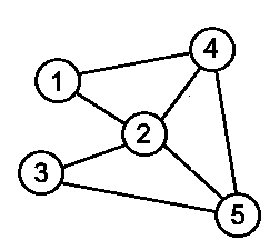
\includegraphics[width=1in]{L3-connectivity.png}
\end{figure}

因此,problem是抽象的表示,instance是具体的实例。

我们一般会碰到两类问题,第一类是优化问题:对这个问题当中任何一个实例(instance)$x \in I$,我们找一个最优的解(solution)$y^*$,如最短路径问题。

\textbf{例2:最短路径问题}

{\bf 输入:}一个图$G=<V,E>$,两个将节点,$s$ 和 $t$;

{\bf 输出:}从$s$ 到 $t$的最短路径,或者返回``NO''如果图中不存在$s$ 到 $t$的路径;

\begin{figure}[H]
	\centering
  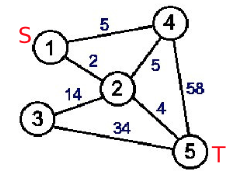
\includegraphics[width=1.0in]{L3-shortestpath.png}
\end{figure}

我们遇到的很多问题都是优化问题,但是优化问题在分析难度时并不容易,因为优化问题需要得到目标函数值。而这里存在一个比较好分析的问题类型,称为判定问题:对于任何一个问题的实例(instance)答案只有$ \texttt{YES, NO} $。

\textbf{例3:路径问题(path problem)}

{\bf 输入:} 一个图 $G=<V,E>$, 两个节点 $s$ 和 $t$, 以及 \textcolor{red}{一个整数 $k$};

{\bf 输出:} 一条从 $s$ 到 $t$ 的路径,并且长度最大为 $k$; 

\begin{figure}[H]
    \centering
    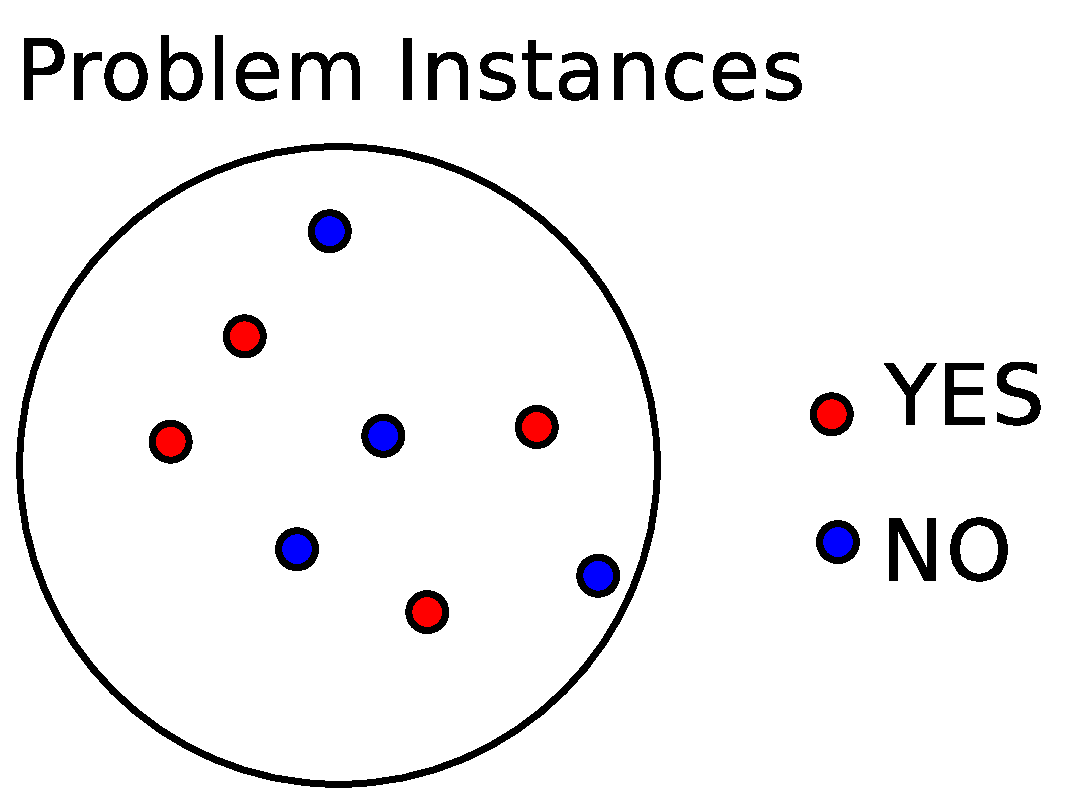
\includegraphics[width=1.5in]{L3-decisionproblem.eps}
\end{figure}

如果我们能找到这条路径回答YES,否则回答NO。我们通过观察可以发现,为优化问题添加一个限制条件,如最大长度不超过$k$等,可以将优化问题转换为判定问题,这样答案简单,便于分析。对于判定问题我们很容易进行一些描述。对例3,我们知道问题就是一堆实例的集合,我们把所有的是实例拿过来放在这里,形成一个文氏图,每个点代表一个实例(instance)。针对每个实例,答案只有两种(Yes or No),这比优化问题描述起来简单多了。

\section{归约}
现在我们对问题怎么表示已经很清楚了,就是把INPUT及OUTPUT描述清楚就行。这个对于同学们没有什么困难,接下来需要考虑的是问题之间的难度关系怎么比较,怎么说一个问题比另外一个问题更难呢?这个办法叫做归约,它的目的是揭示两个问题之间的关系,就是比较两个问题谁难谁容易。我们看一下详细的归约是什么意思。

\subsection{多项式时间归约}

多项式时间的归约是一个变换的过程,我们记作$f$,它把问题A的任何一个实例(instance)$\alpha$都能快速变成问题B的一个实例$\beta=f(\alpha)$,变换$f$包含两点要求:

1.快速变换:变换过程只需要花费多项式时间。

2.等价性:变换前后答案需要相同。(如果实例$\alpha$答案是YES,则实例$\beta=f(\alpha)$答案也应为YES。)

我们将满足上述两点要求的过程记作$A \leq_P B$,读作``\textcolor{red}{\bf A is reducible to  B  }''。

那么上面的符号都代表什么意义呢?$P$是polynomial,代表多项式时间,$\leq$看作两个问题之间的难度关系,如$A \leq_P B$表示$B$比$A$更难。

\subsection{多项式时间归约的图形表示及其意义}

上述多项式时间归约的定义可以用如下图所示的文氏图来表示:

\begin{figure}[H]
    \centering
    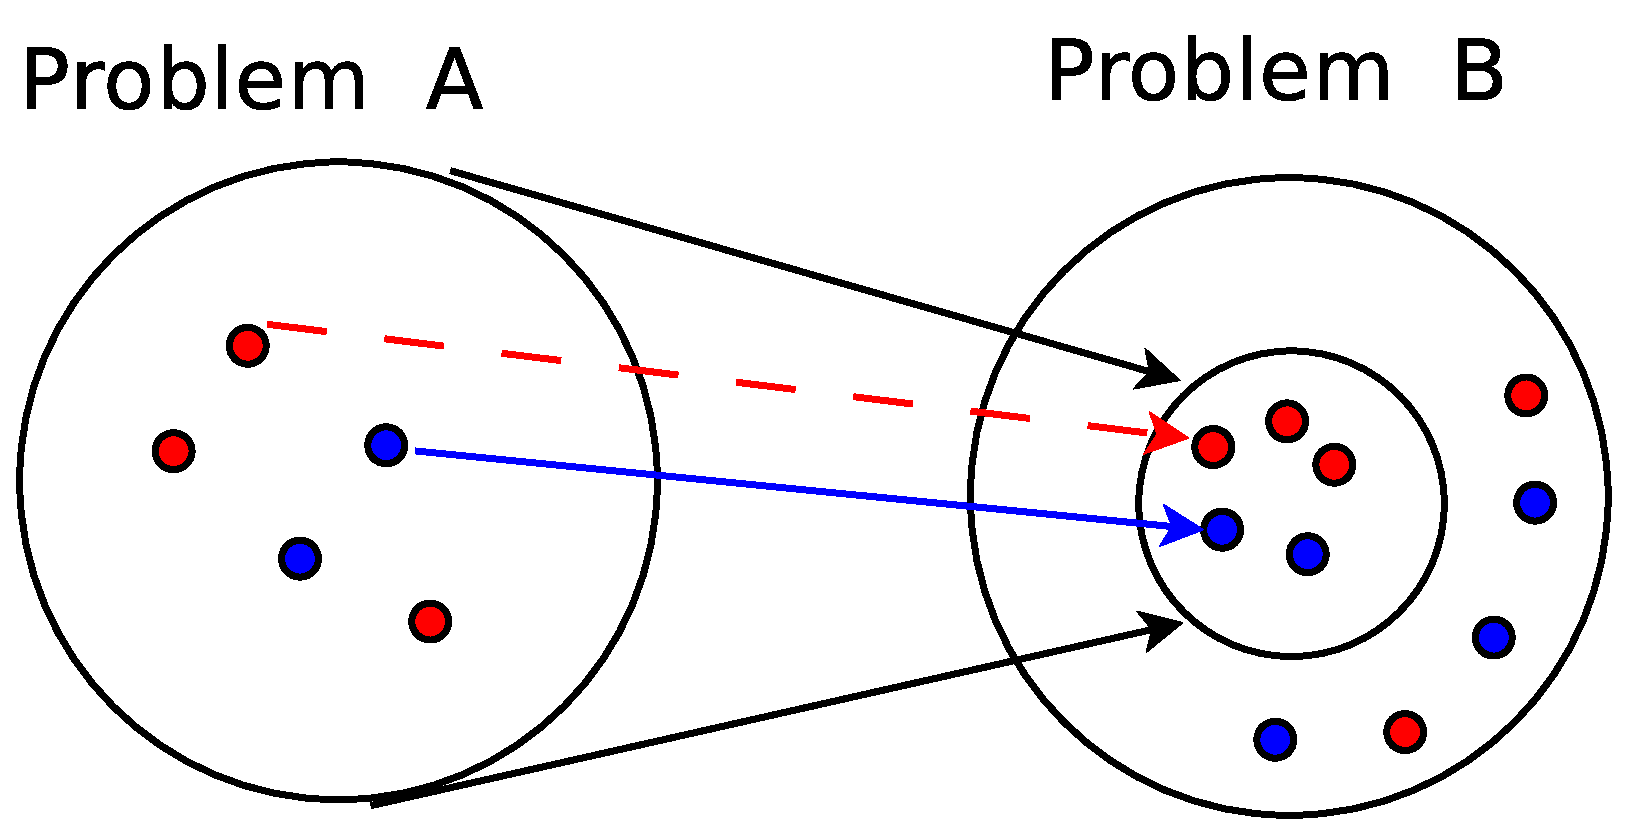
\includegraphics[width=2in]{L3-reduction.eps}
\end{figure}

问题A可以用一个圈表示一个集合,里面包含问题A的所有实例,每个实例的答案只有YES或NO,归约就是能够把问题A中的任意一个实例变作问题B中的一个实例,这样我们就把A中的每个实例映射到B中的实例上,值得注意的是,如果A的某个实例答案是YES,则相应的映射到B中的实例答案也必须是YES,A中实例答案是NO则映射的实例的答案也必须是NO。

到现在为止我们只介绍了问题之间怎么进行归约,接下来将要解释为什么归约之后就可以认为$B$比$A$更难。

\textbf{定理1}:如果问题B能在多项式时间内求解,则问题A也能在多项式时间内求解。

我们可以证明这个定理,但是我们先看它反过来的定理。

\textbf{定理2}:相反的,如果问题A是难的,则问题B也是难的。

所以我们可以说问题$B$比问题$A$难,那么为什么说定理1是对的呢?假如说我们对问题B有个快速求解的算法,则我们能得到一个A的快速求解算法,即给定一个问题A的实例$\alpha$,首先通过多项式时间归约将实例$\alpha$转换成问题B的实例$\beta=f(\alpha)$,运行问题B的快速求解算法我们就可以得到实例$\beta$的答案。最后根据等价性,可以通过$\beta$的答案得到问题A的实例$\alpha$的答案。

抽象的东西讲的太多了,接下来看一下实际的例子。

\section{归约举例}
在分析这个问题之前插一句话,今天这堂课非常强调大家数学建模的能力,强调数学建模能力有三个地方。第一个是线性规划,我们需要将一个实际问题抽象成一个线性规划,第二个是网络流,很多问题可以转换成网络流问题,第三个就是将要讲的这个。我们首先训练一下如何将一个实际问题抽象出来。所以接下来大家会看到很多的名词和很多问题的抽象定义,但是大家不要怕,我们都会讲一个实际的问题是什么。
\subsection{{\sc IndependentSet} $\le_P$ {\sc VertexCover}}
\subsubsection{独立集问题}

我们先看什么是独立集问题,先不管抽象的定义,先看实际的需求,假设我们有$n$个朋友,但是有些朋友之间相处不好,容易发生冲突。那么如何在避免人际关系紧张的前提下邀请至少k个朋友吃饭。我们将这个实际问题抽象成一个数学问题。

 {\bf 输入:} 给定一个图 $G=<V,E>$, 和一个整数 $k$;

 {\bf 输出:} 是否存在一个点的集合 $S  \subseteq V$, $|S| = k$, 使得集合$S$中任意两点都没有边相连?

我们用每个点表示一个人,如果两个人关系不好则在图中用一条边连接两个点,则可以用下图表示7个人的人际关系图,问如果要请3个人吃饭,请哪些人。

\begin{figure}[H]
\centering
\begin{tikzpicture}[scale=1.1, auto,swap]
    % Draw a 7,11 network
    % First we draw the vertices
    \foreach \pos/\name in {{(0,2)/v1}, {(2,2)/v2}, {(1,1)/v3}, {(2,1)/v4}, {(3,1)/v5}, {(0,0)/v6}, {(2,0)/v7}}
        \node[smallvertex] (\name) at \pos {};
        
    % Connect vertices with edges and draw weights
    \foreach \source/ \dest /\weight in {v1/v2/{}, v1/v3/{}, v2/v3/{}, v2/v4/{}, v2/v5/{}, v3/v6/{}, v3/v7/{}, v6/v7/{}, v4/v7/{}, v5/v7/{}  }
        \path[undirectededge] (\source) -- node[weight] {$\weight$} (\dest);
%       \draw[dashed, ->] (0,0) arc  (120:60:2);

      \end{tikzpicture}
\end{figure}
问题很清楚了,就是给我们一个图,在图中找k个节点,使得各个节点间没有边连接,我们称这样的点的集合为独立集,独立的意思是说两个点之间没有边。我们看看其他的情形

$k=3$:蓝色标示的三个节点是独立的。
\begin{figure}[H]
\centering
\begin{tikzpicture}[scale=1.1, auto,swap]
    % Draw a 7,11 network
    % First we draw the vertices
    \foreach \pos/\name in {{(0,2)/v1}, {(2,2)/v2}, {(1,1)/v3}, {(2,1)/v4}, {(3,1)/v5}, {(0,0)/v6}, {(2,0)/v7}}
        \node[smallvertex] (\name) at \pos {};
        
    % Connect vertices with edges and draw weights
    \foreach \source/ \dest /\weight in {v1/v2/{}, v1/v3/{}, v2/v3/{}, v2/v4/{}, v2/v5/{}, v3/v6/{}, v3/v7/{}, v6/v7/{}, v4/v7/{}, v5/v7/{}  }
        \path[undirectededge] (\source) -- node[weight] {$\weight$} (\dest);
%       \draw[dashed, ->] (0,0) arc  (120:60:2);


    \foreach \pos/\name in { {(1,1)/v3}, {(2,1)/v4}, {(3,1)/v5}}
        \node[blue smallvertex] (\name) at \pos {};
      \end{tikzpicture}
\end{figure}
上面这个情况大家一眼就可以看出来,那么出现如下所示的情形呢。

$k=8,k=9$:蓝色的节点形成一个独立集,左边8个节点,右边9个节点。

\begin{figure}[H]
	\centering
	\begin{minipage}{0.45\textwidth}
 		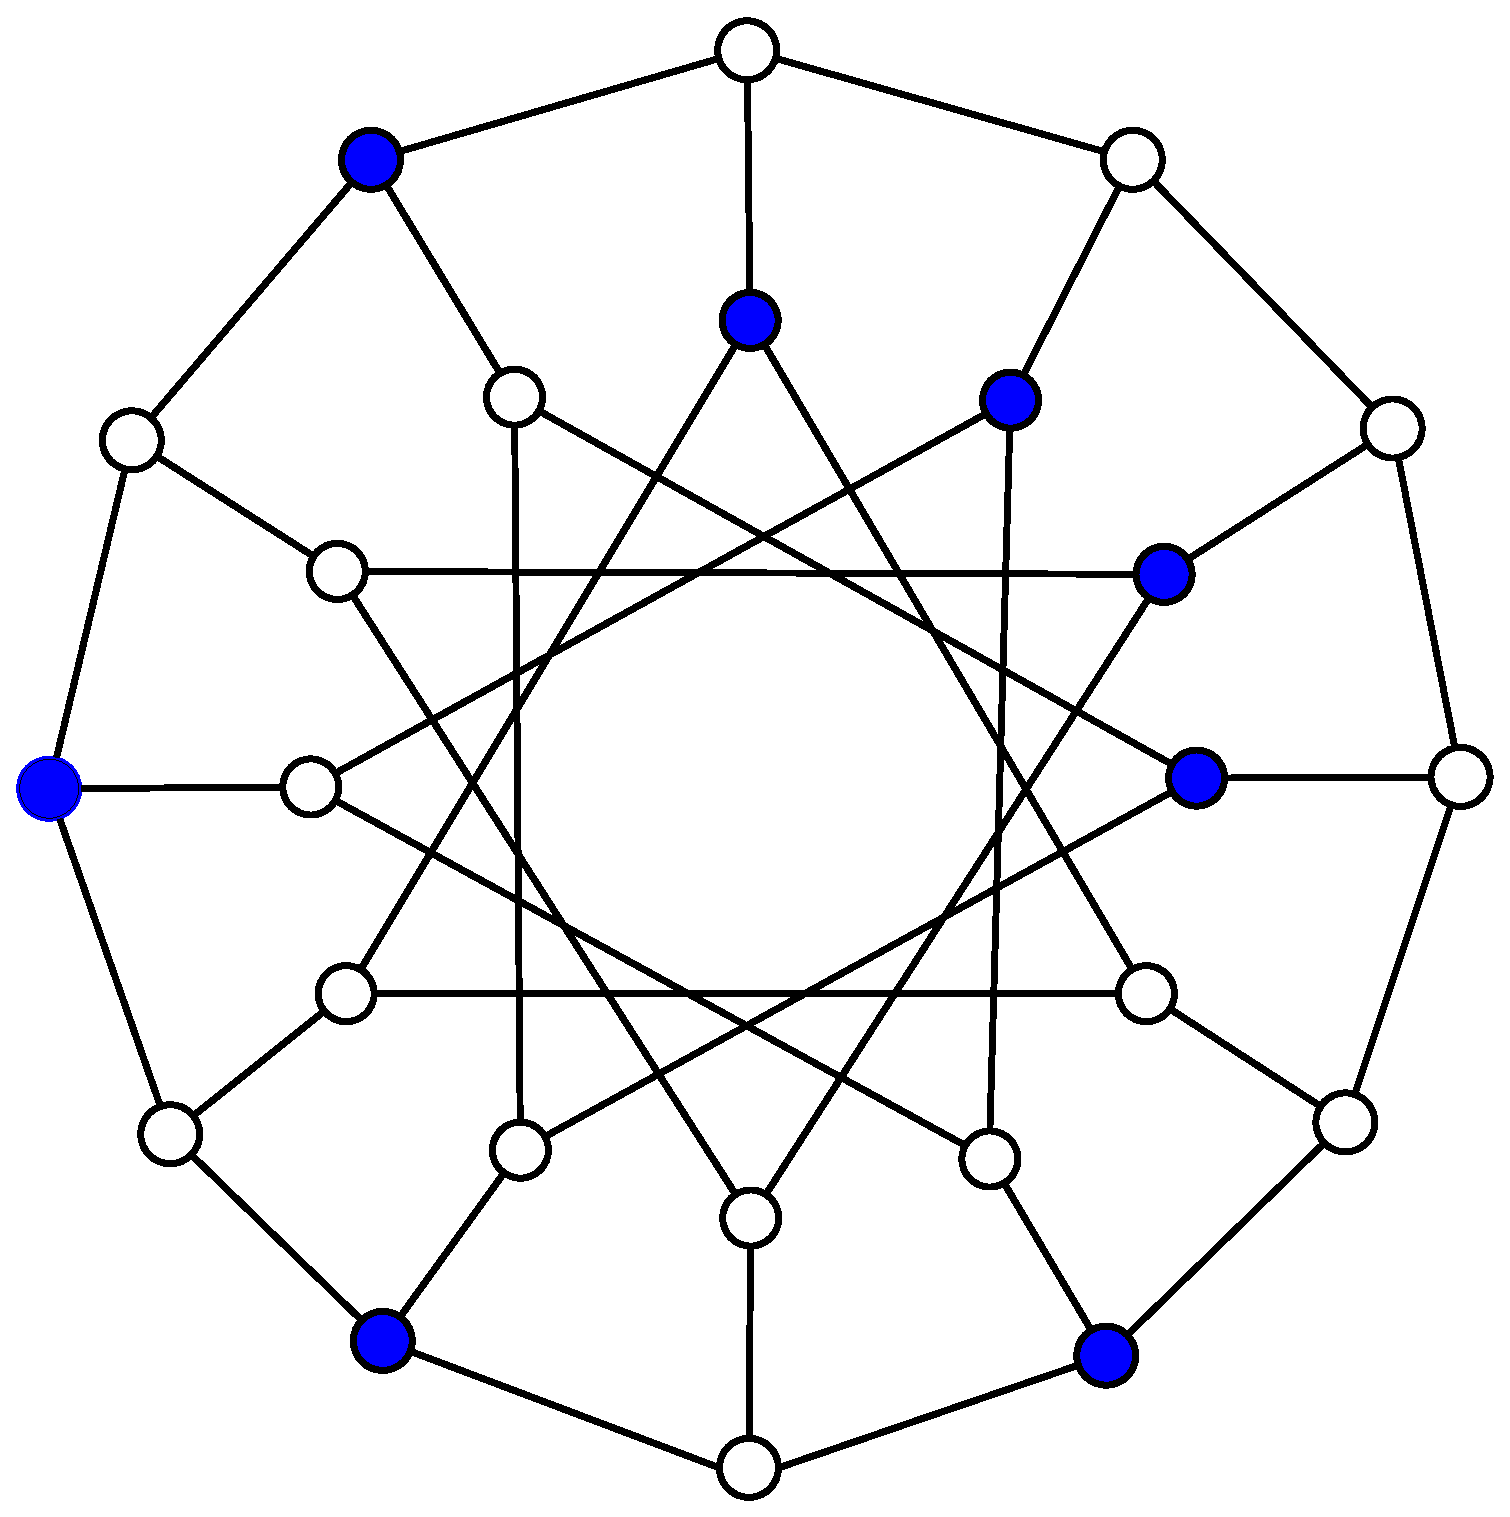
\includegraphics[width=\textwidth] {L3-independentsetgraph24-8.eps} 
 	\end{minipage}
	\begin{minipage}{0.45\textwidth}
 		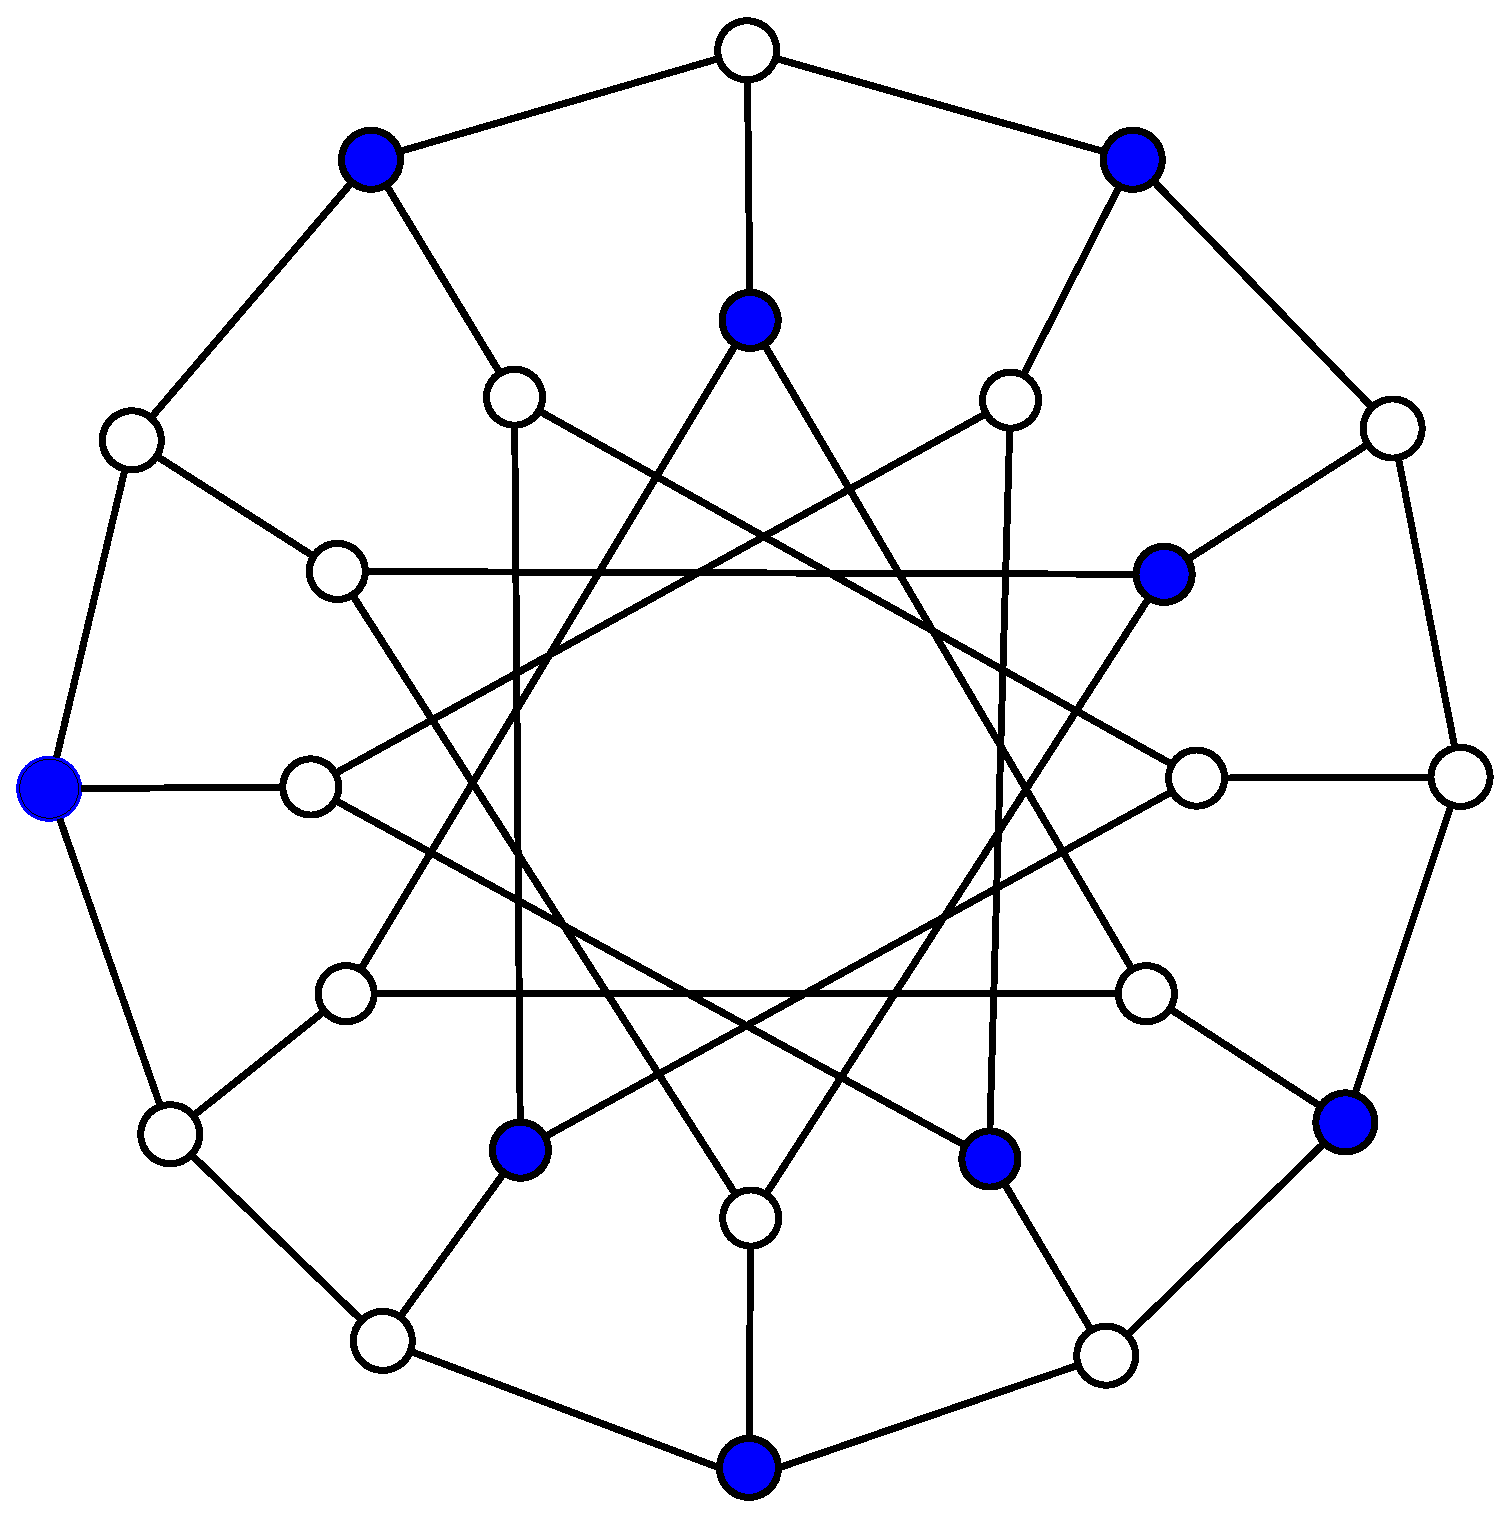
\includegraphics[width=\textwidth] {L3-independentsetgraph24-9.eps} 
	\end{minipage}
\end{figure}
左边的图是非常非常有名的图,让我们在中间请8个人吃饭,怎么请。这幅图是这么画的,外面是12个点,如同时钟,里面也是12个点,每个都连接一条边,里面的点之间画了三角形,总共4个三角形。这幅图可以表示请八个人吃饭,也可以表示请九个人吃饭。我们可以验证,蓝色的任意两个点之间不存在边连接。大家先不慌问怎么找出来的,这个不好找。这个图找10个人就不可能了,虽然你有24个点,找不出10个人。

\subsubsection{顶点覆盖问题}

介绍完独立集问题再来介绍顶点覆盖问题。那么什么是顶点覆盖呢,还是先不看抽象的定义,先看现实的一个例子。我们有n个地点,每个地点之间有一条道路,问如何挑选地点安装摄像头使得我们可以监控所有的道路。这是一个很实际的例子,我们不可能给所有的道路安装摄像头,肯定是要尽可能少的使用摄像头。

我们可以把这个实际问题抽象成一个数学问题。

 {\bf 输入:} 给定一个图 $G=<V,E>$, 和一个整数 $k$;

 {\bf 输出:} 是否存在点的集合 $S  \subseteq V$, $|S| = k$,使得任意一条边至少能被一个节点覆盖(cover)? 

 以下图为例,我们可以找到4个节点(用红色标注)覆盖所有的边。

\begin{figure}[H]
\centering
\begin{tikzpicture}[scale=1.1, auto,swap]
    % Draw a 7,11 network
    % First we draw the vertices
    \foreach \pos/\name in {{(0,2)/v1}, {(2,2)/v2}, {(1,1)/v3}, {(2,1)/v4}, {(3,1)/v5}, {(0,0)/v6}, {(2,0)/v7}}
        \node[smallvertex] (\name) at \pos {};
        
    % Connect vertices with edges and draw weights
    \foreach \source/ \dest /\weight in {v1/v2/{}, v1/v3/{}, v2/v3/{}, v2/v4/{}, v2/v5/{}, v3/v6/{}, v3/v7/{}, v6/v7/{}, v4/v7/{}, v5/v7/{}  }
        \path[undirectededge] (\source) -- node[weight] {$\weight$} (\dest);
%       \draw[dashed, ->] (0,0) arc  (120:60:2);

    \foreach \pos/\name in { {(1,1)/v3}, {(2,1)/v4}, {(3,1)/v5}}
        \node[blue smallvertex] (\name) at \pos {};

    \foreach \pos/\name in { {(0,2)/v1}, {(2,2)/v2},  {(0,0)/v6}, {(2,0)/v7}}
        \node[red smallvertex] (\name) at \pos {};
      \end{tikzpicture}

\end{figure}

\subsubsection{归约——变换}

那么这两个问题我们解释的很清楚了,一个问题是请客吃饭,一个问题是装摄像头。我们为什么可以说装摄像头问题比请客吃饭问题要难呢?要证明这个观点,我们需要构造一个变换,使得独立集问题中的每个实例$<G, k>$都可以转换成顶点覆盖问题中的实例$<G', k'>$,并且对应问题的答案一致。

接下来我们看怎么构造这样的变换。原先的请客吃饭问题(独立集问题)给了我们一个人际关系图,每个节点代表一个人,假如左边的图代表请客吃饭问题的一个实例,我们把它变成如右图所示的装摄像头问题的一个实例。请客吃饭问题的实例是一个人际关系图,装摄像头问题的实例是地点和道路之间的关系图。

\begin{figure}[H]
	\centering
 	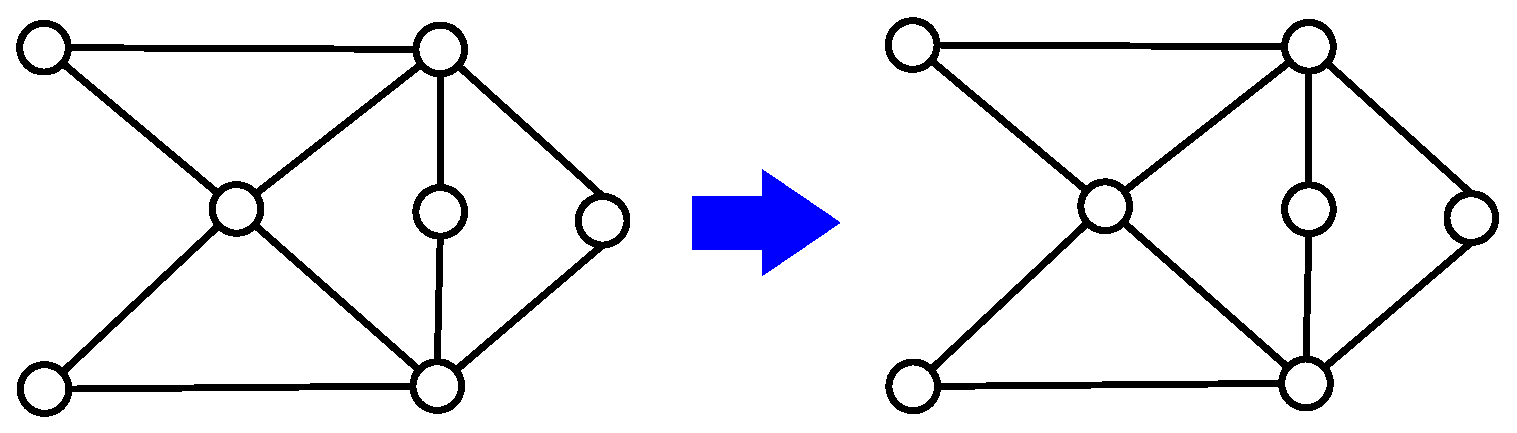
\includegraphics[width=3in]{L3-independentsettovertexcover.eps}
\caption{Transformation from an {\sc Independent Set} instance $(G, k=3)$ into a {\sc Vertex Cover} instance $(G'=G, k'=4)$}
\end{figure}

那么我们怎么构造一个装摄像头问题的关系图呢,针对这个问题很简单,直接将人际关系图复制作为装摄像头问题的关系图。但是我们需要注意到,问题里不仅需要定义一个图,还需要定义一个参数$k$,那么$k$怎么定义呢。对于原始的请客吃饭问题是需要我们请$k$个人,而装摄像头问题需要我们找$n-k$个地方装摄像头。

正如图中的那句话所说:变换过程将独立集问题变换成顶点覆盖问题,并且图还是那个图,但是独立集问题$k=3$,顶点覆盖问题$k'=n-k=7-3=4$

\subsubsection{归约——等价性}

现在变换过程有了,我们需要证明等价性。

\textbf{定理:}图$G$ 有独立集 $S$ ($|S|=k$) $\Leftrightarrow$ $G'$ 有顶点覆盖集 $S'$ ($|S'|=n-k$). 

用通俗的话说就是,我们能请$k$个人吃饭,当且仅当我们能在装摄像头问题中找到$n-k$个节点装摄像头覆盖到所有的边。

为什么呢,我们这么看。假如说对原始的请客吃饭问题,我们回答一个YES,即能找到k个人一起吃饭,且不会发生冲突,我们把这些人叫做$s$(蓝色标注)。如下图中找到的三个人不会发生冲突,因为对于任意的一条边$e=(u,v)$,假设两个端点是$u$和$v$,则两个端点不会同时在$S$中,因此可以得到$u \in V-S$ 或者 $v \in V-S$。我们定义$S'=V-S$(红色标注),我们就在这些地方装摄像头。在图中可以表示我们请蓝色节点代表的朋友吃饭,而在剩下的红色节点代表的地方装摄像头覆盖所有的边。因为蓝色节点之间没有边,则剩下的红色节点肯定可以覆盖所有的边。

\begin{figure}[H]
 	\centering
 	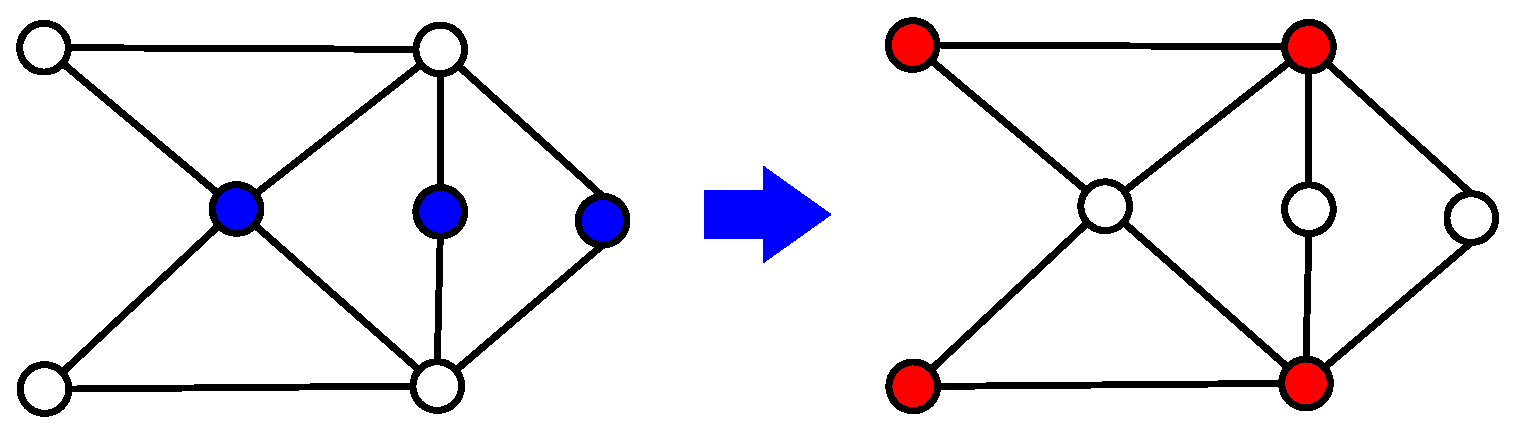
\includegraphics[width=2.4in]{L3-independentsettovertexcoverredblue.eps}
 	\caption{ {\small The complement of an  independent set(in blue) form a vertex cover (in red)} } 
\end{figure}

在构建快速的变换过程以及证明等价性之后,我们就证明了装摄像头问题(顶点覆盖问题)比请客吃饭问题(独立集问题)要难。实际上请客吃饭问题就足够的难,它属于NP类问题中最难最难的一类问题。我们也可以证明独立集问题比顶点覆盖问题要难,即两个问题的难度系数是一样的,这个问题我们以后再说。

刚才的例子让我们知道了怎么说明一个问题比另一个问题更难。但是因为分析问题的复杂度有时候会比较麻烦,因此这个例子的分析可能会给大家带来困扰。我们来看看牛人C. Papadimitriou是怎么分析问题的难度,怎么做归约的:

{\it 
要证明一个问题是NP完全的,我们可以从问题的简单实例开始仔细琢磨,直到我们找到一个小例子,它表现出非常有趣的行为。有时候,对这个例子的观察可以直接得到一个NP完全问题的简单证明.... 有时候称其为``机关建设''。
}

(Excerpted from Computer and Complexity)

\subsection{{\sc Vertex Cover} $\le_P$ {\sc Set Cover}}
再来看一个简单的归约,集合覆盖问题比顶点覆盖问题还要难。

\subsubsection{集合覆盖问题}

对于集合覆盖问题,我们来看一个实际例子。IBM公司要开发一个杀毒软件,杀毒软件识别病毒是通过检查代码中是否存在某些关键字,每种病毒都有特殊的关键字,但是任何一种关键字可能对应很多种病毒。为了降低杀毒软件病毒库的大小,我们感兴趣的是能不能找出有代表性的关键字,而不是每种病毒都单独对应一个关键字。我们来看一下它抽象成什么问题。

{\bf 输入:} 一个集合$U$ 有 $n$ 个元素,一些$U$的子集 $S_1, S_2,...,S_m$,和一个数$k$. 

{\bf 输出:} 能否找到 $k$ 个子集,使得它们的并集等于全集$U$?

我们来举个简单的例子解释这个问题。

\begin{figure}[H]
	\centering
	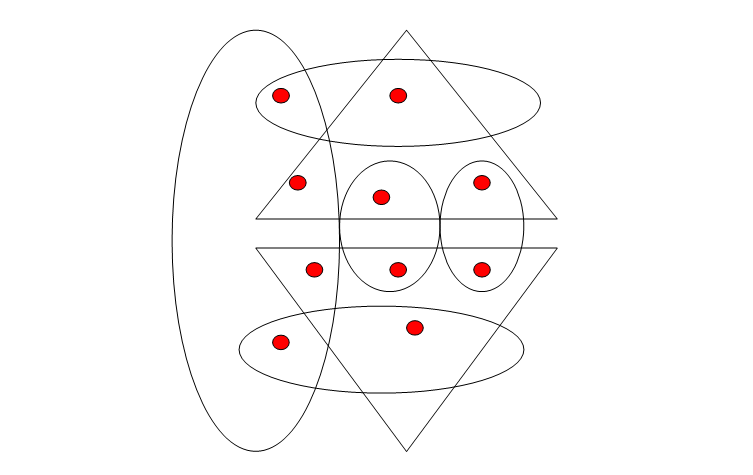
\includegraphics[width=2in]{setcover1.png}
 % setcover1.eps: 22002048x0 pixel, 300 dpi, 186284.00x0.00 cm, bb=14 14 407 318
\end{figure}

在这个实例中我们假设有10个病毒,每个病毒用一个红点表示,每个框表示一个关键词,表示包含在框内的病毒共享这个关键词,扫描病毒时发现这个关键词,我们就知道是框内的某个病毒出现。我们的目标是找尽可能少的子集使得所有的病毒都包含在这些框内,这样我们就能减少病毒库的规模,而在这个例子中我们能找到最少3个集合使得它们的并集能够包含所有红点。而这个就是集合覆盖问题中“覆盖”一词的实际意义,即子集的集合能将所有红点包含在内。

在弄清楚集合覆盖问题后,我们需要证明集合覆盖问题比顶点覆盖问题要难。

\subsubsection{归约——变换,等价性}

我们首先构造一种变换,即任何一个道路和地点的连接图我们总能变换成杀毒的事情,怎么变。假如原先的地方有四个地点,连接图如下图左边所示,令$k=2$,则我们可以找出两个地方覆盖所有的道路。我们就把这个实例变换成杀毒的问题的一个实例,即连接图中的每条边对应一个病毒(右图中的点)。左图中1号顶点能覆盖边$e1$,$e3$两条边,则在右图中构造一个集合覆盖顶点$e1$和$e3$,同理左图中3号顶点能覆盖边$e2$,$e3$和$e4$,我们同样在右图中构造一个集合覆盖这些点,以此类推。所以如果我们能在左图中找到两个点覆盖所有的道路,则必定可以在右图中找到两个集合覆盖所有的病毒(点)。因此如果我们顶点覆盖问题的实例回答YES,则我们同样可以在集合覆盖问题中找到相应的解,使得答案同样是YES,使得该变换满足等价性。

\begin{figure}[H]
	\centering
	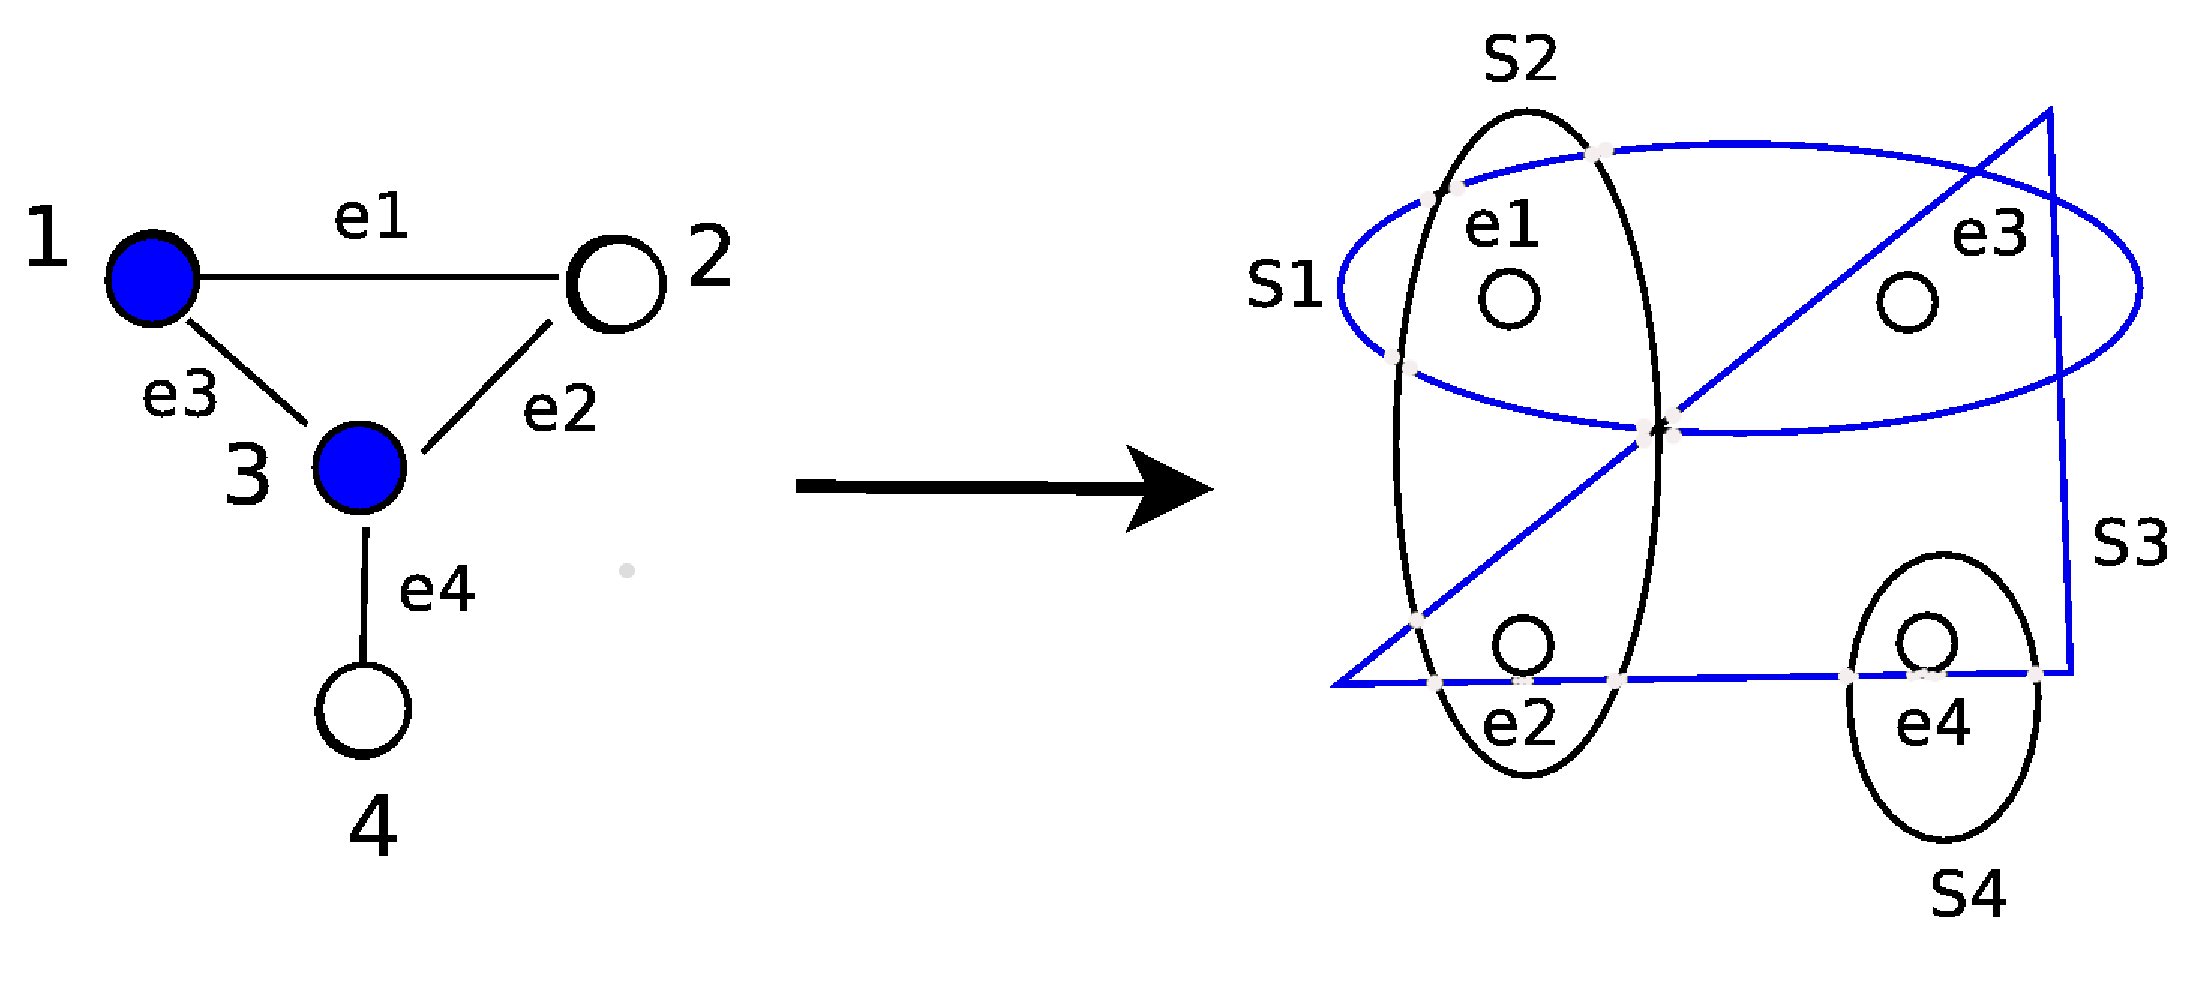
\includegraphics[width=2.8in]{L3-vertexcoversetcover.eps}
 % setcover1.eps: 22002048x0 pixel, 300 dpi, 186284.00x0.00 cm, bb=14 14 407 318
\end{figure}

上面这个简单的例子是让大家熟悉一下什么时候归约,下面我们讲一个稍微难点的例子。

\subsection{通过 ``Gadget''归约: {\sc 3-SAT} $\le_P$ {\sc Independent Set}}

观察了两个简单的归约之后,我们来看一个不是那么直接的归约问题,独立集问题比3-SAT问题更难。

\subsubsection{{ SAT (Satisfiability)} Problem}

什么是3-SAT?3-SAT问题是数理逻辑中很重要的一个问题,很基本的一个问题。很多实际的问题都能转换成3-SAT问题,它的全称是可满足性问题。在人工智能领域表达一组变量的约束,或者在超大规模集成电路测试时验证电路是否符合需求方面等问题都可以转换成3-SAT问题。

我们来看一下可满足性问题的定义。这个定义稍微有点繁琐,大家耐心往下看。

{\bf 输入:} 给定一个合取范式(CNF) $\phi = C_1 \wedge C_2 ... \wedge C_k$;

{\bf 输出:} 是否存在对所有变量$x_i$的一个合适赋值,使得所有的子句 $C_j$ 都是$\texttt{TRUE}$(可满足)? 

\textbf{\textcolor{red}{注意:}}

1.布尔变量: $x_1, x_2, ..., x_n$, $x_i = \texttt{TRUE/FALSE} $;

2.文字(项): 一个变量 $x_i$, 或者它的非 $\neg x_i$,表示一个文字;

3.子句: 一些文字的或: $C_1 = x_1 \vee \neg x_2 \vee ... \vee x_3 $;

4.合取范式(CNF): 一系列子句的与 $\phi = C_1 \wedge C_2 ... \wedge C_k$;

我们来看一个例子来理解这个定义。

CNF:  $(x_1 \vee \neg x_2) \wedge ( \neg x_1 \vee \neg x_3 ) \wedge ( x_2 \vee \neg x_3 )$;

\texttt{TRUE} assignment:  $x_1 = \texttt{FALSE}, x_2= \texttt{FALSE}, x_3 = \texttt{FALSE} $;

上面这个例子的合取范式由三个子句组成,第一个子句是$x_1 \vee \neg x_2$,第二个子句是$\neg x_1 \vee \neg x_3$,第三个子句是$x_2 \vee \neg x_3$。三个子句之间用$\wedge $(与)进行连接,这就形成了一个输入。因此我们的目标对布尔变量的值进行一种组合,使得三个子句都等于TRUE。而当$x_1 = \texttt{FALSE}, x_2= \texttt{FALSE}, x_3 = \texttt{FALSE} $时我们可以验证三个子句均等于TRUE,从而合取范式也等于TRUE,即这个输入是可满足的。


我们对SAT问题有两种看法,让我们找一堆TRUE和FALSE的赋值组合,使得整体等于TRUE,这个求解过程可以从两个角度来思考。第一个角度是从变量的角度来思考,我们可以尝试变量为TRUE或FALSE,从而找到一种组合使得所有子句都等于TRUE;第二个角度是从子句的角度来思考,我们假设每个子句都等于TRUE,则我们从每个子句中选择一个或多个布尔变量为TRUE,使得该子句为TRUE(因为子句是一些文字的或,所以只要有一个文字为TRUE则该子句为TRUE),但是我们从每个子句中挑选的布尔变量之间不能发生冲突(如第一个子句$x_1=\texttt{TRUE}$,则第二个子句\textcolor{red}{不能选择}$\neg x_1 = \texttt{TRUE}$)。

\subsubsection{SAT问题与独立集问题之间的联系}

谈到冲突,大家可能联想到请客吃饭的问题,实际上与请客吃饭问题是类似的。有了这点知识,我们就可以证明请客吃饭比SAT问题要难。

在证明过程中我们需要一点精巧设计的零件(gadget)。在这里我们先回顾一下gadget的定义:一个很小的,非常有用的,精巧设计的机关或工具;有明确定义的功能,可以用来模拟另外一个问题。例如我们可以人际关系图来模拟SAT问题中的变量或者子句。在请客吃饭问题中,输入是一个人际关系图,在这里我们设计一个非常巧妙的人际关系图,就是一个三角形,三个人之间任意两个之间都有矛盾,所以如果我们请这三个人吃饭,则只能选择其中一人,右图中也是同样的。

\begin{figure}[H]
	\centering
	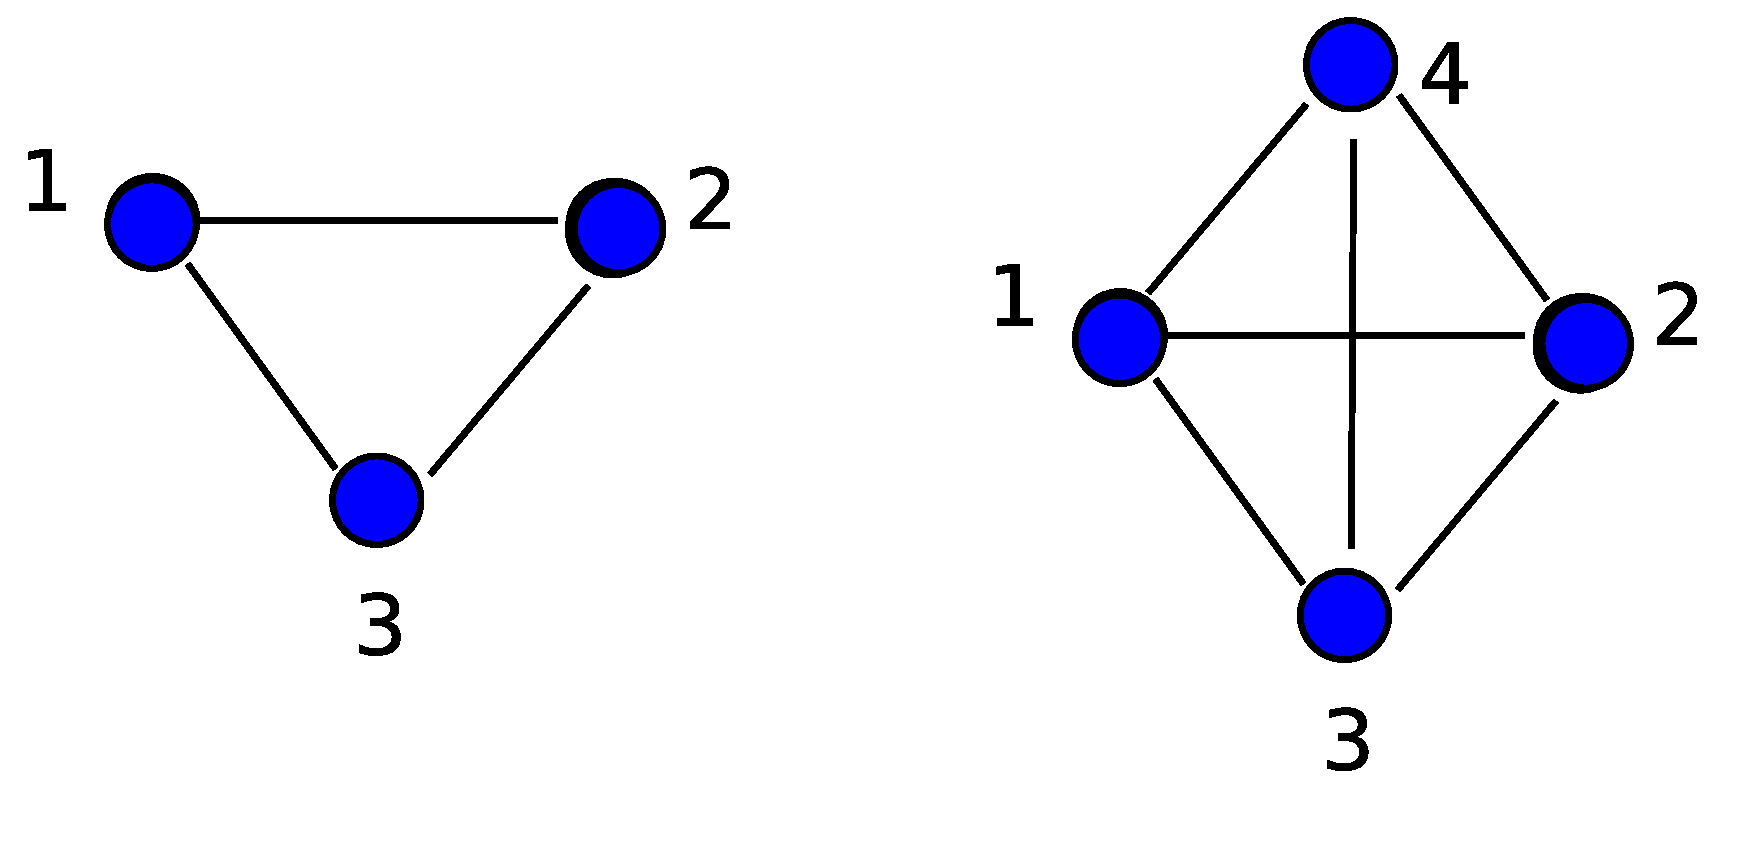
\includegraphics[width=1.9in]{L3-clique.eps}
\end{figure}

大家注意我们刚才的描述中就暗含了$or$这种关系在里面。事实上,在SAT问题中子句内的变量是通过或进行相连,即逻辑关系中核心是或关系。而在人际关系图中,我们同样可以在图中表示或关系,即在左图中我们可以\textcolor{red}{\bf 选择 1 或 选择 2 或 选择 3} ,所以实质上是一样的。换句话说如果我们画一个三角形就能模拟出or的关系了,所以逻辑关系我们可以用逻辑变量来表示,也可以用画一幅图来表示。

\subsubsection{归约——变换}

基于这个认识,我们就可以把SAT问题的任何一个实例变成一个人际关系图。假如一个SAT实例是$(x_1 \vee x_2 \vee x_3) AND (\neg x_1 \vee x_5 \vee x_6)$,所以我们需要找一个对变量的赋值方案,使得第一个子句为TRUE,第二个子句也为TRUE。我们可以把它表示成如下图所示的独立集问题。

\begin{figure}[H]
\centering
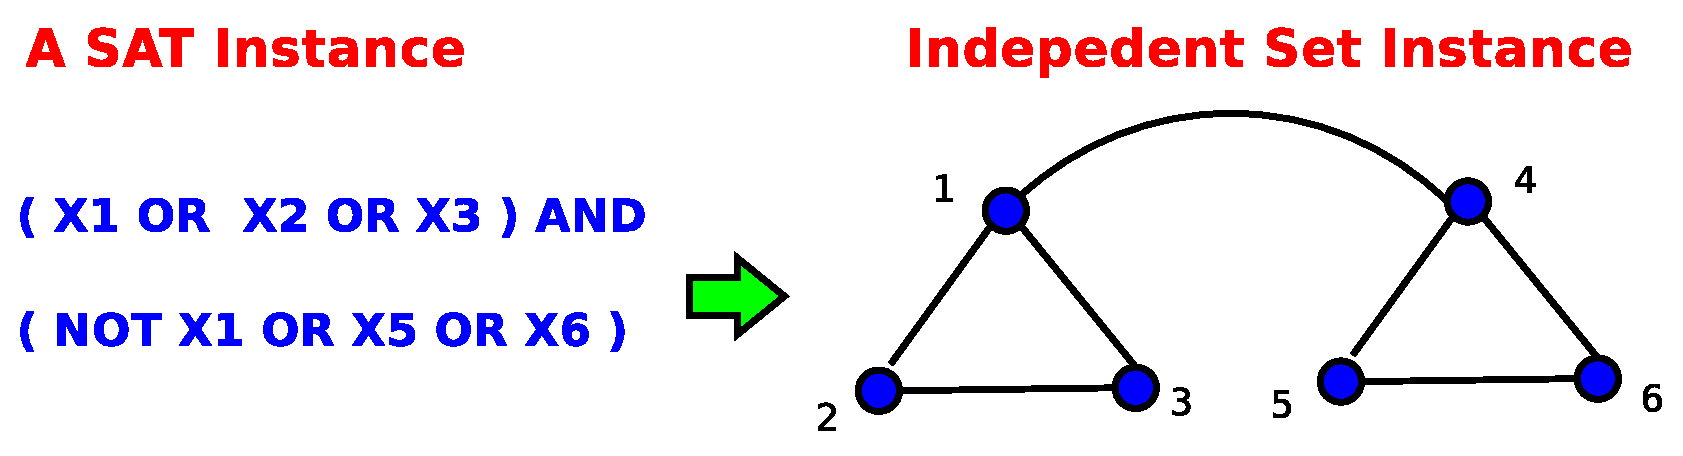
\includegraphics[width=3in]{L3-satindependentset.eps}
\end{figure}

我们来观察一下是怎么变换的,在这边$x_1$对应人际关系图中$1$号点,$x_2$对应2号点,$x_3$对应3号点,然后我们先添加一个4号点,然后$x_5$,$x_6$分别对应一个点。需要注意的是,在右图中画了两个三角形,以第一子句为例,子句的逻辑关系是$x_1$或$x_2$或$x_3$,而右图第一个三角形同样表示要么选1号,要么选2号,要么选3号。另外$x_1$对应1号,而$x_4$对应$\neg x_1$,所以在右图中我们可以在$x_1$和$x_4$之间连一条边,表示要么选$x_1$,要么选$x_4$,即如果$x_1 = \texttt{TRUE}$则$\neg x_1 = \texttt{FALSE}$。

我们从分析中可以看出来,这样的变换是非常简单的,每个子句对应一个三角形,同时在$x_i$和$\neg x_i$之间连一条边。

\subsubsection{归约——等价性}

现在我们就可以证明这个问题了。假如说在SAT问题中存在一种赋值安排,使得问题的答案为TRUE,则在请客吃饭问题中肯定可以找两个人吃饭,而不会发生冲突。

\begin{figure}[H]
\centering
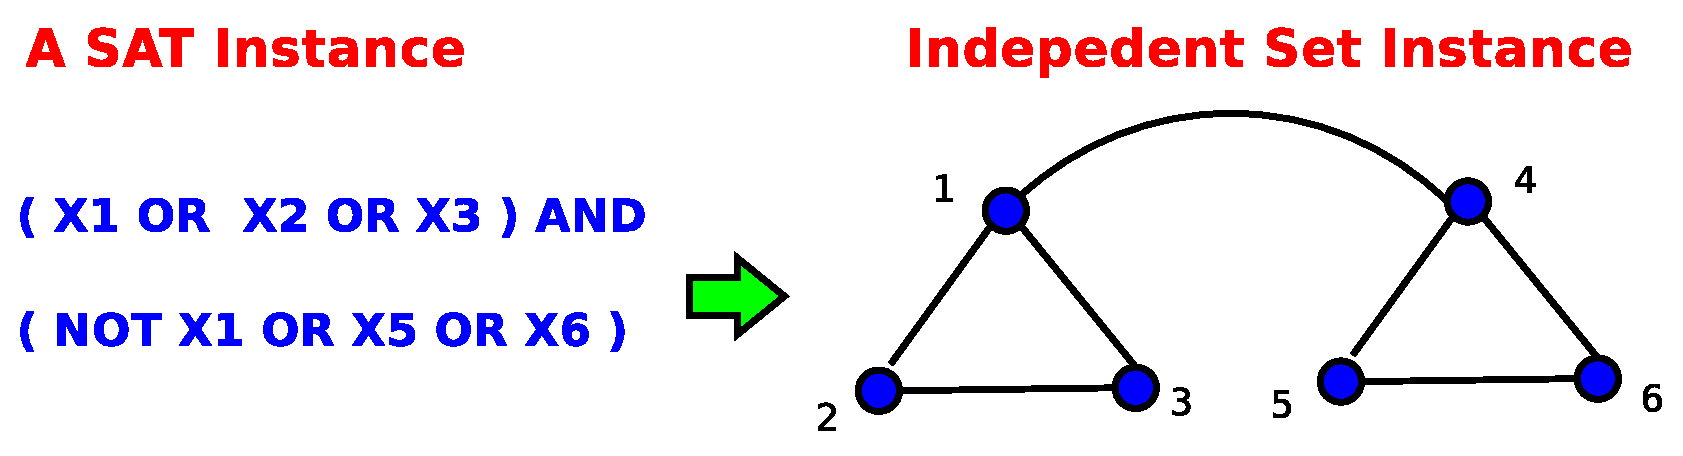
\includegraphics[width=3in]{L3-satindependentset.eps}
\end{figure}

我们来看看证明为什么是这样的。假如这个例子是可满足的,则必定存在一种赋值安排使得每个子句都等于TRUE(只安排一个文字等于TRUE),所以我们就选等于TRUE的文字所对应的节点,且节点之间不会发生冲突。所以我们只要选那些使得问题可满足的文字的对应节点就不会发生冲突。

现在我们考虑反过来证明这个观点。假如构造的图中我们能请两个人吃饭,则对应的文字的赋值必定是可满足的。因为这些图都是精心构造的图,是一堆的三角形把它们连起来的,每个三角形里面最多最多选一个人,现在我们需要选两个人吃饭,则我们只好在左边的三角形选一个人,右边的三角形选一个人。现在我们假设请$x_1$和$x_6$吃饭,显然是不会发生冲突的,则我们相应的令$x_1 = \texttt{TRUE},x_6 = \texttt{TRUE}$,其余没选的等于$\texttt{FALSE}$,然后我们将这些赋值代入两个子句中,则显然两个子句均等于TRUE。

那么这个核心在哪呢?核心有两点,第一点是我们一定要构造三角形,这就是所谓的“Gadget”,一种非常精巧的结构,保证如果我们选择两个人,则每个三角形必定选一个。第二点是$x_i$和$\neg x_i$有边存在,一定不会同时选。这个例子大家回去再看一下,我们先往下走。

\subsection{通过 ``Gadget''归约: {\sc SAT } $\le_P$ {\sc Hamilton Cycle}}

下面我们同样利用精心构造的东西来证明哈密尔顿圈问题比SAT问题要难。

\subsubsection{哈密尔顿圈}

什么是哈密尔顿圈?哈密尔顿圈是英国的威廉·哈密尔顿爵士在1857年发明的一款游戏,这个游戏的图如下图所示。

\begin{figure}[H]
\centering
  \subfigure{ 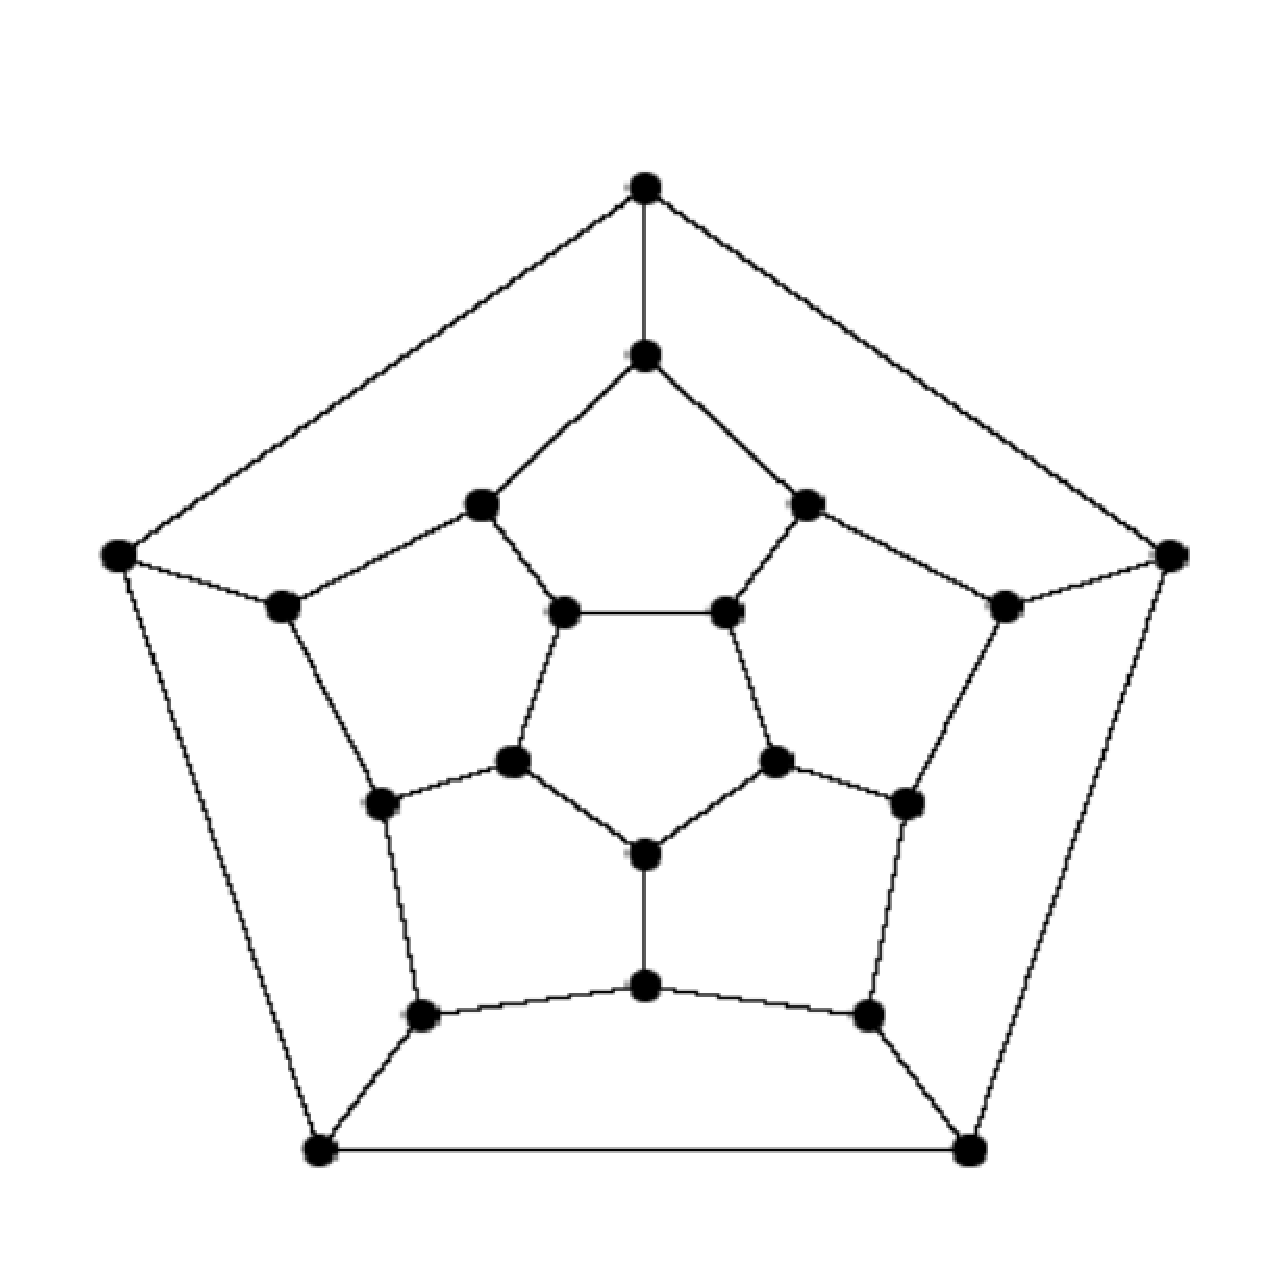
\includegraphics[height=1.3in]{L3-hamiltoncyclegame.eps} } 
  \subfigure{ 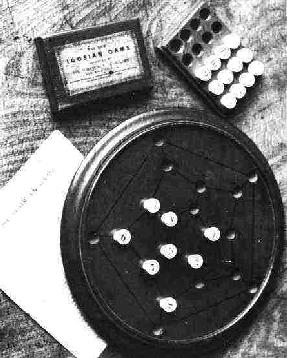
\includegraphics[height=1.3in]{L3-hamiltoncyclegameboard.png} }
\end{figure}

大家注意左图是一幅非常有名的图,这幅图是怎么画的呢?我来给大家演示一下。这个图有个名称,叫Iconian(正十二面体顶点图),即将正十二面体投影到平面上形成的图。它的外边是一个五边形,里边也有一个五边形,然后外面的五边形和里面的五边形之间也会构造成五边形。下面我们给出哈密尔顿圈的抽象定义。

{\bf 输入:} 给定一个图 $G=<V,E>$;

{\bf 输出:} 是否存在一个环路使得该路径经过图中所有的节点,且每个节点只经过一次?

虽然这个图已经很有规律了,但是并不容易找到这样的路径,所以这个问题是挺难的一个问题。但是它是可以存在一条满足要求的环路的,结果如左图图所示。

\begin{figure}[H]
\centering
  \subfigure{ 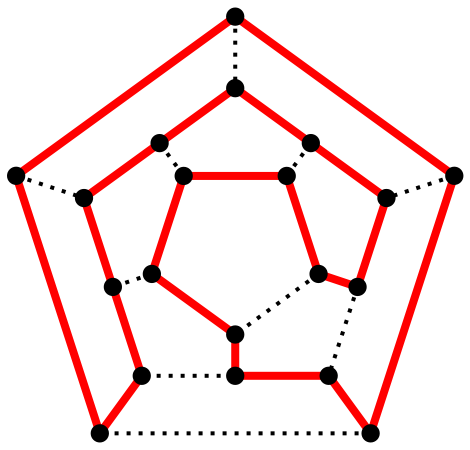
\includegraphics[height=1.5in]{L3-hamiltoncycleexample1.png} } 
  \subfigure{ 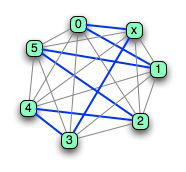
\includegraphics[height=1.5in]{L3-hamiltoncycleexample2.png} } 
\end{figure}

我们从左图可以得知它是存在哈密尔顿圈的,而右图是一幅没有规律的图形,它也存在一个哈密尔顿圈。但是大家知道左图是一幅非常规整的图,而右图也是凑巧找到一个。现在如果给我们一般一幅图,问能否画出满足要求的环路。大家会觉得不知道怎么做,会很难。但是这个问题会非常非常有用,在这里我插入一点其他的知识。

\subsubsection{哈密尔顿圈应用——人类基因组测序}

我们人类基因组测序,就完全得益于对这个问题的快速求解。那么什么叫DNA测序呢?我们人体内的遗传物质是染色体,染色体的核心是DNA,DNA是双螺旋结构,由两条链构成,彼此之间是互补链,因此我们只要知道其中一条链就可以了。我们体内是23条染色体,加起来是3Gb大小,也就是说平均下来每个都很长。DNA其实类似字符串,是由$A,T,C,G$四个字母组成的很长的字符串。

\begin{figure}[H]
\centering
 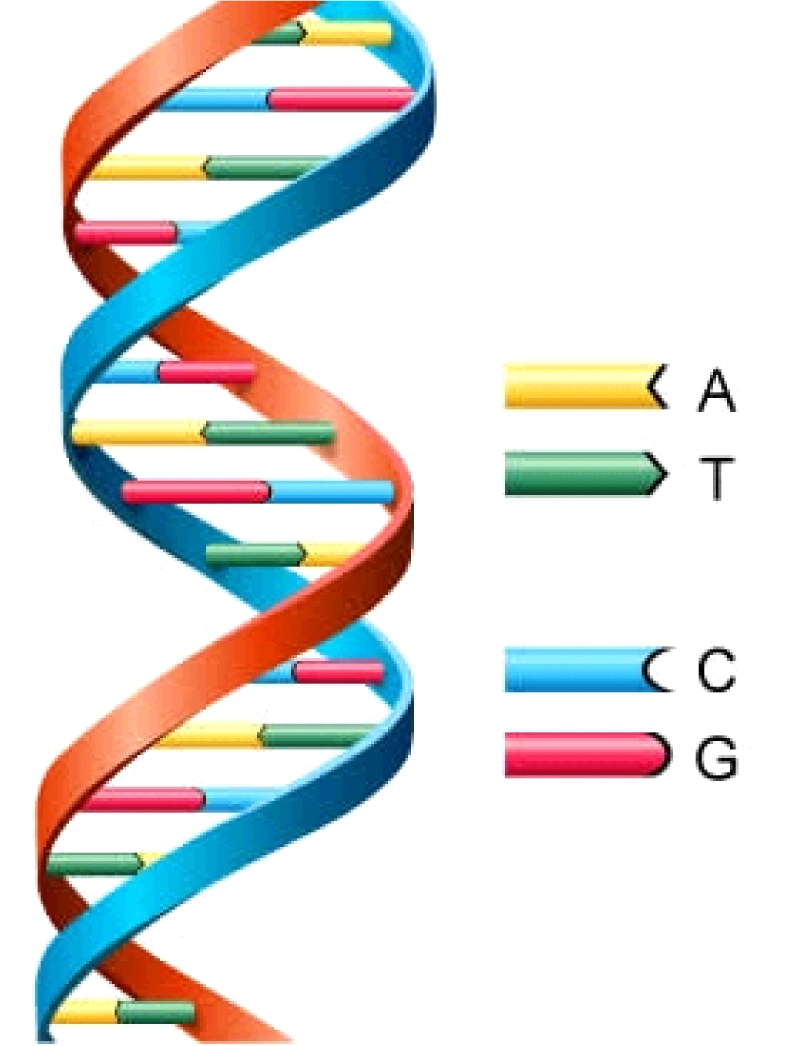
\includegraphics[width=0.5in]{L3-DNA.png}
\end{figure}
\begin{figure}[H]
\centering
 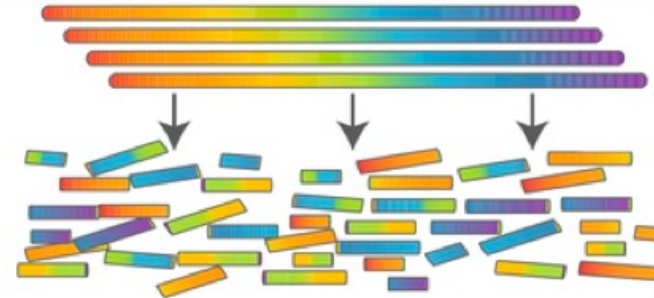
\includegraphics[width=2in]{L3-dnasequencing.png}
\end{figure}

那人类基因组测序是什么意思呢?就是希望得到DNA链的碱基排列顺序。一开始由生物学家发起成立的国际组织——人类基因组联盟(HGP),他们首先将很长的DNA链人工进行切分成很短很短的DNA序列,然后将这些很短的DNA序列分配给各个国家进行同步测序。与此同时,有一位叫Venter的人也在同步开展这项工作,不同的是他把DNA链用超声波随机的进行切分测序,然后转换成哈密尔顿路径问题,交给超级计算机进行求解运算,从而得到完整的DNA链的碱基序列。下面我们介绍一下第二种方法。

我们假设细菌的基因组如图a所示,是一个环状的,然后把它随机的打断。例如从A处打断,一直到T,则会形成$ATGGCGT$这样的一个DNA片段。然后构造如图b的一幅图,每个节点就是一个片段,如果一个片段的尾巴和另一个片段的头重合了,就在两个节点之间连一条边。现在节点和边都有了,寻找完整的DNA链的碱基序列,就可以转换成在图中找一个环路,使得路径经过所有节点,且每个节点只经过一次,这样哈密尔顿圈就对应了基因组。

\begin{figure}[H]
\centering
 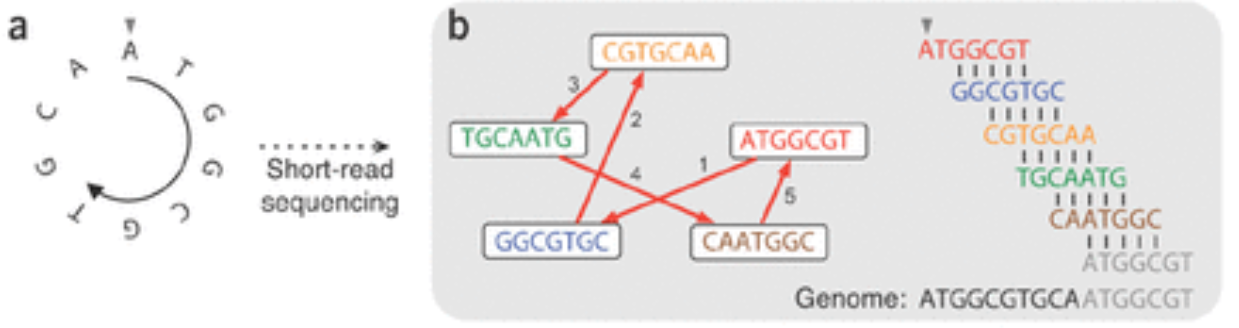
\includegraphics[width=4in]{L3-GenomeAssembly.png}
\end{figure}

\subsubsection{哈密尔顿圈问题与SAT问题之间的联系}

这个问题很难,上面的DNA片段装配问题往往需要利用超级计算机才能完成。人们认为哈密尔顿圈问题比SAT问题还要难,这是为什么呢?我们先来观察一些小的例子,最后从中识别出一些特定的属性,就如同之前的几个例子中表现的那样。

\begin{figure}[H]
\centering
 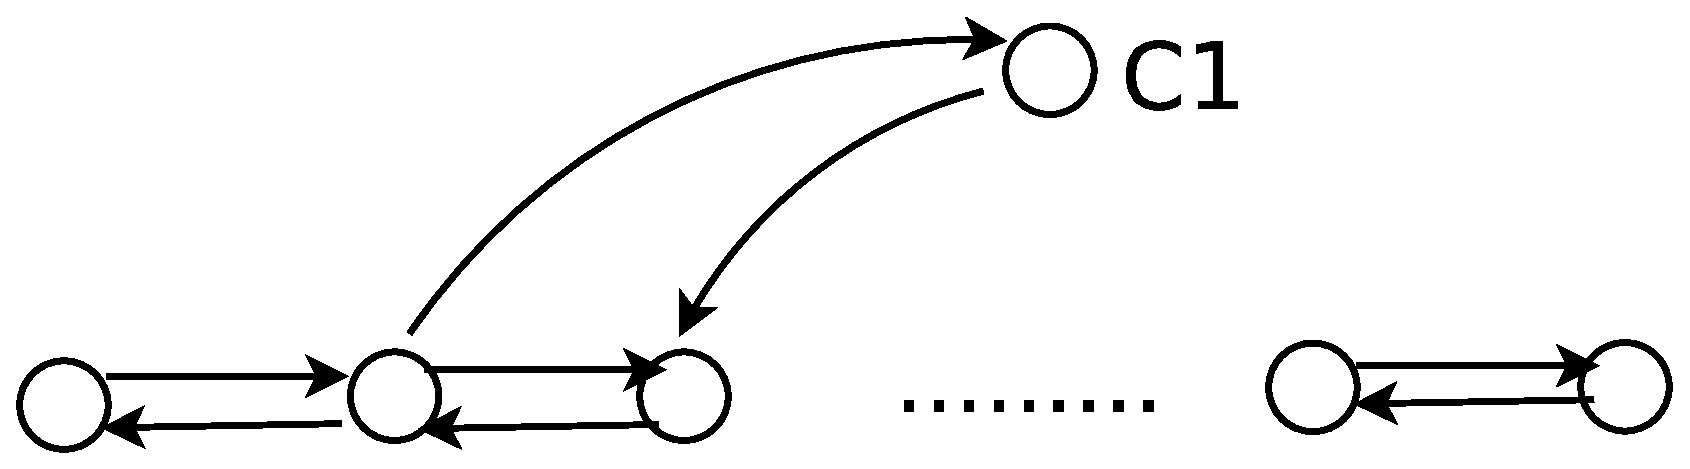
\includegraphics[width=2in]{L3-sathamiltongadgetsnocolor.eps}
\end{figure}

现在我们来观察一个例子。这个例子中画了一排的节点(先不考虑$C_1$节点),节点之间双向连接。现在假如需要我们遍历所有的节点,且每个节点只能经过一次,我们需要怎样遍历?第一种方法,从最左边的节点向右走,直到最右端的节点,这样我们就遍历了所有节点一次且仅有一次,我们先不考虑回来的问题;第二种方法,从右往左走,直到最左边的节点,这样我们遍历了所有节点一次且仅有一次。那么如果我们选择从中间出发,则必然会发生一个节点经过两次的情况。

所以想要经过所有的节点且每个节点只经过一次,只有两种方案,要么从最左边走到最右边,要么从最右边走到最左边,而不能从中间开始。

我们可以注意到在上面这段话中蕴含着\textcolor{red}{或(or)关系}。现在我们在图中再加入一个点$C_1$,并进行如上图所示的连接。那么针对这种情况,如何做到遍历所有的点且每个点只经过一次?刚才已经分析过,如果只是底下的一排节点,则要么从最左边开始从左往右,要么从最右边开始,从右往左。现在我们从右边尝试一下,但是如果我们要经过$C_1$,则必然发生一个节点经过两次这种情况。那我们只好从左边开始遍历,很容易验证存在一条路径,它能够遍历所有的点,且所有节点只遍历一遍。

\begin{figure}[H]
\centering
 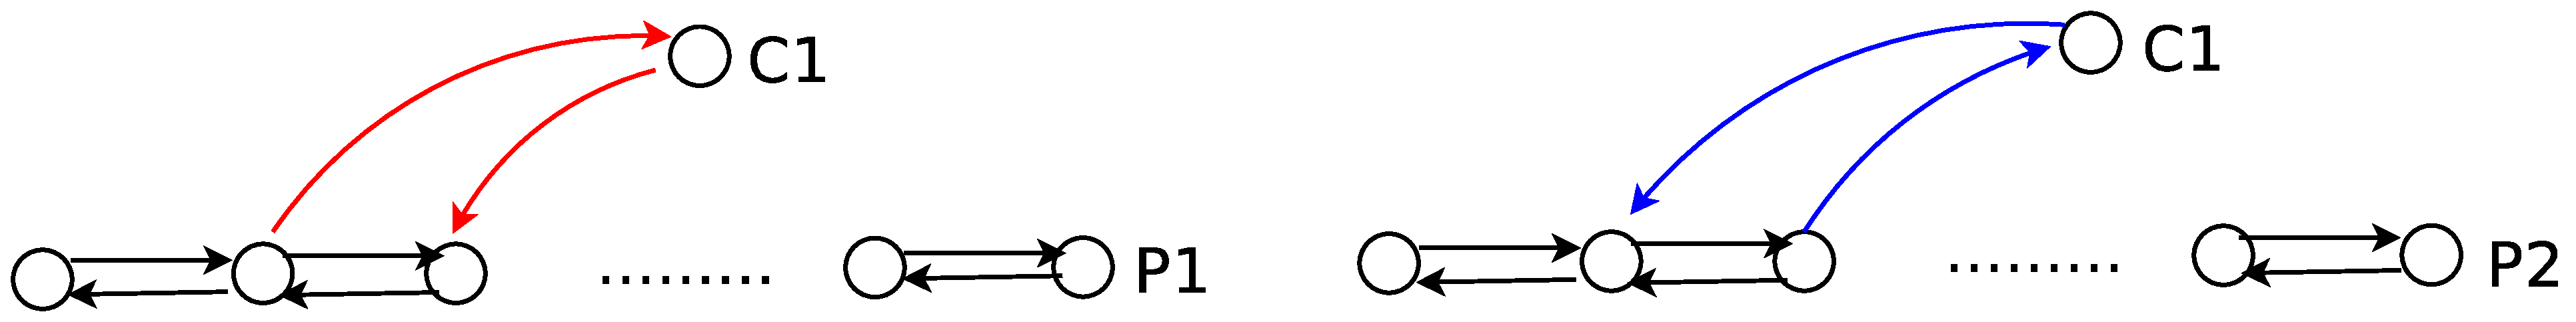
\includegraphics[width=4.0in]{L3-sathamiltongadgets.eps}
\end{figure}

如P1所示精心构造的小零件,使得原来或的关系,变成只能按照一个方向走。如果我们想从右往左遍历,则可以按P2的方式构造这个图,将连接$C_1$节点的路径方向反转一下即可,这样只能选择从右往左走遍历所有节点。

\subsubsection{归约——变换}

现在我们构造了一个小的零件,可以用路径选择方式来表示或关系,而SAT问题里面同样存在或关系。在图中我们可以用从左往右走还是从右往左走来表示或关系。这样我们就可以构造一个变换,即对任何一个SAT问题的实例,就可以构造一个哈密尔顿圈实例。我们用下面这个实例来说明怎么构造这样一幅图。

下图中SAT实例是$X_1$ OR NOT $X_2$ OR $X_3$,我们这么来构造相应的图。任何一个变量对应一排节点,即$X_1$对应第一排的节点,$X_2$对应第二排的节点,$X_3$对应第三排的节点。整个图是一个子句,我们构造一个特殊的节点$C_1$表示这个子句,如果子句中包含$X_j$,则第$j$排节点按顺时针方向连接$C_1$节点(如下图中第1,3排节点),如果子句中包含$\neg X_j$,则第$j$排节点按逆时针方向连接$C_1$节点(如下图中第2排节点),再构造两个节点$S$和$T$。现在来看整体是个什么样子,第一个变量构造一排的节点,一排要么从左往右走,要么从右往左走。如此,我们不妨规定,从左往右走相应的布尔变量(不是子句中的文字的取值)取\texttt{TRUE},从右往左走相应的布尔变量(不是子句中文字的取值)取\texttt{FALSE}。

\begin{figure}[H]
\centering
 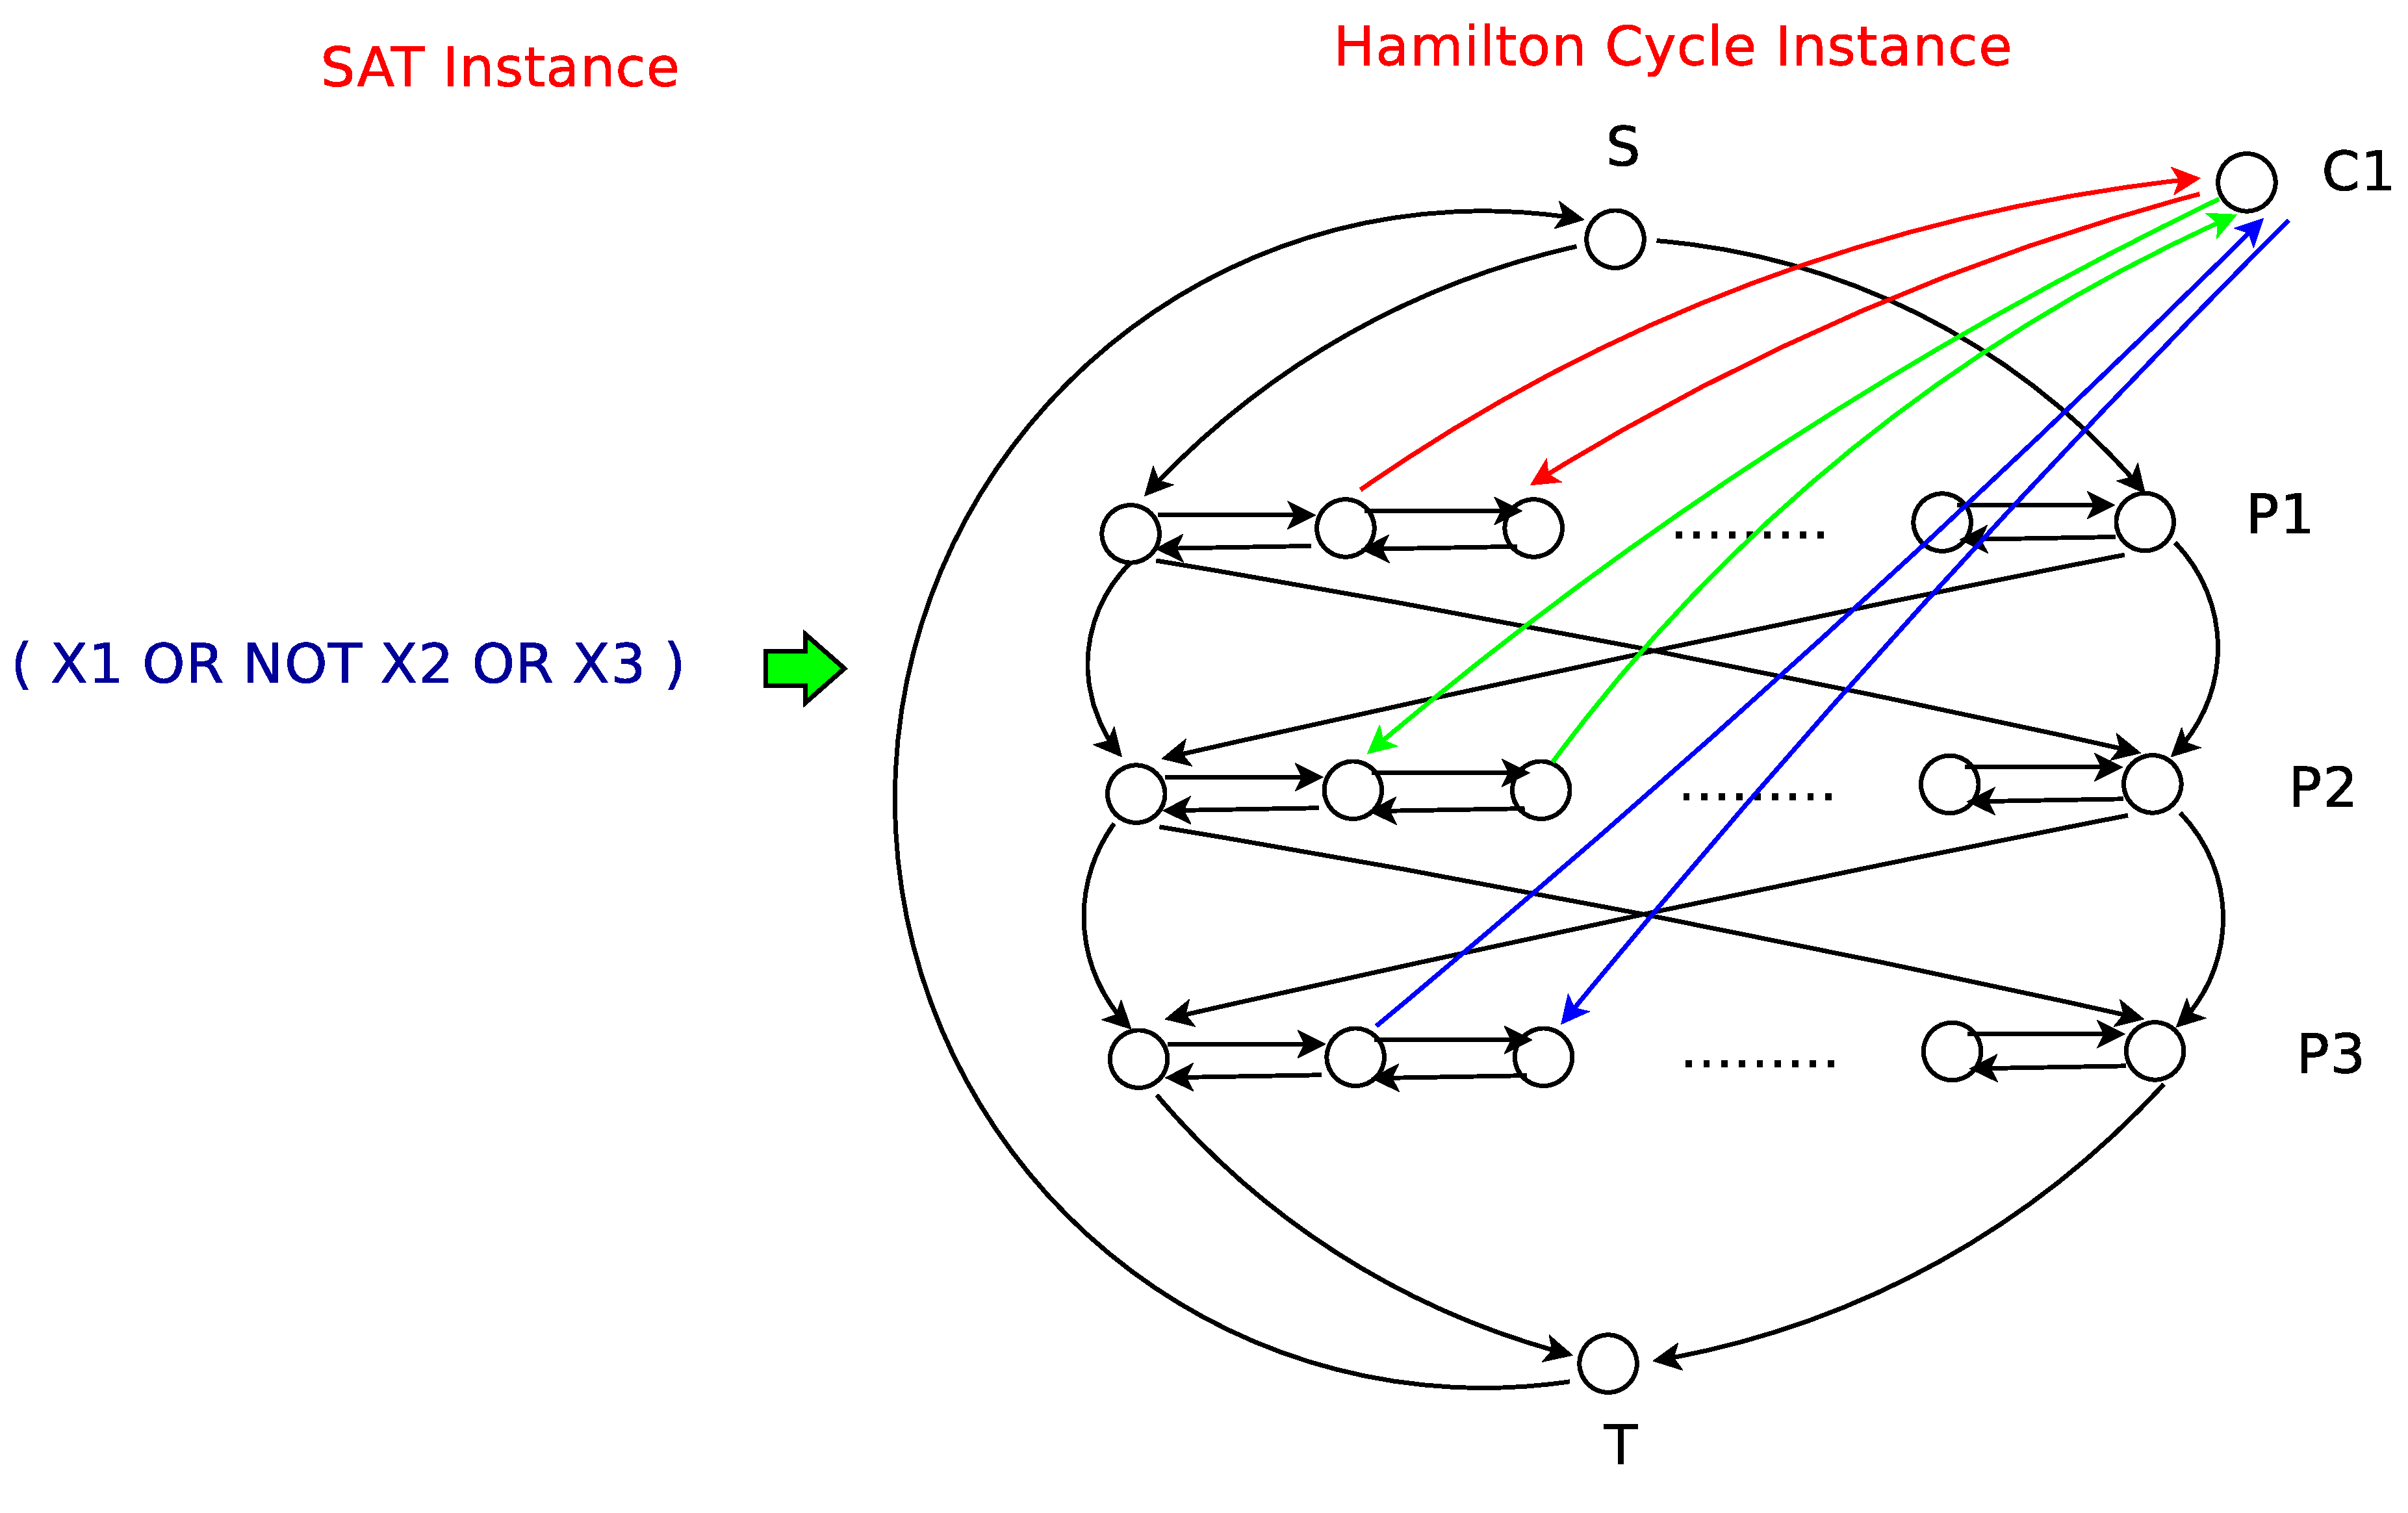
\includegraphics[width=3in]{L3-sathamilton.eps}
\end{figure}

现在这幅图我们分解出来一层一层的看,第一层是$X_1$一排的节点,第二层是$X_2$一排的节点,第三层$X_3$一排的节点。我们从点$S$出发,经过所有的节点,即$S$可以连接到第一排最左边的节点,然后往右走,也可以指向第一排最右边的节点然后往左走。假如从$S$节点走到第一排的最左边的节点,然后往右走走到最右边的节点,接下来如果第二排是从右往左走则直接连接下面的节点,下一排也可能从左往右走,则我们需要将第一排最右边的节点连接到第二排最左边的节点,类似的,第一排的最左边的节点也要连到第二排最左边的节点和第二排最右边的节点,因为我们并不知道第一排会选择从哪个方向走。路径最终指向节点$T$,$T$再回来连接到$S$,这样就可以了。

还有这个$C_1$,这个$C_1$我们必定要走,怎么办呢?此时我们令子句中的每个文字都等于TURE,假定第一排从左往右走,$X_1 = \texttt{TRUE}$,则我们可以沿着红色的路径经过$C_1$。第二排表示$\neg X_2 = \texttt{TRUE},X_2 = \texttt{FALSE}$,所以我们从右往左走,然后沿着绿色的路径经过$C_1$。我们令$X_3 = \texttt{TRUE}$,则我们选择沿着蓝色的路径经过$C_1$。这样对任何一个SAT问题的实例,我们构造了一个如上图所示的稀奇古怪的图。

如果对原始问题有个TRUE赋值,即使得子句结果为TRUE,则我们在图中一定可以找到一个圈。如果原始问题有个FALSE赋值,则在图中一定不存在一个圈,我们来看看为什么。子句TRUE赋值,我们可以令$X_1 = \texttt{TRUE}, X_2 = \texttt{FALSE}, X_3 = \texttt{TRUE}$,则子句整体都等于TRUE。

\begin{figure}[H]
\centering
 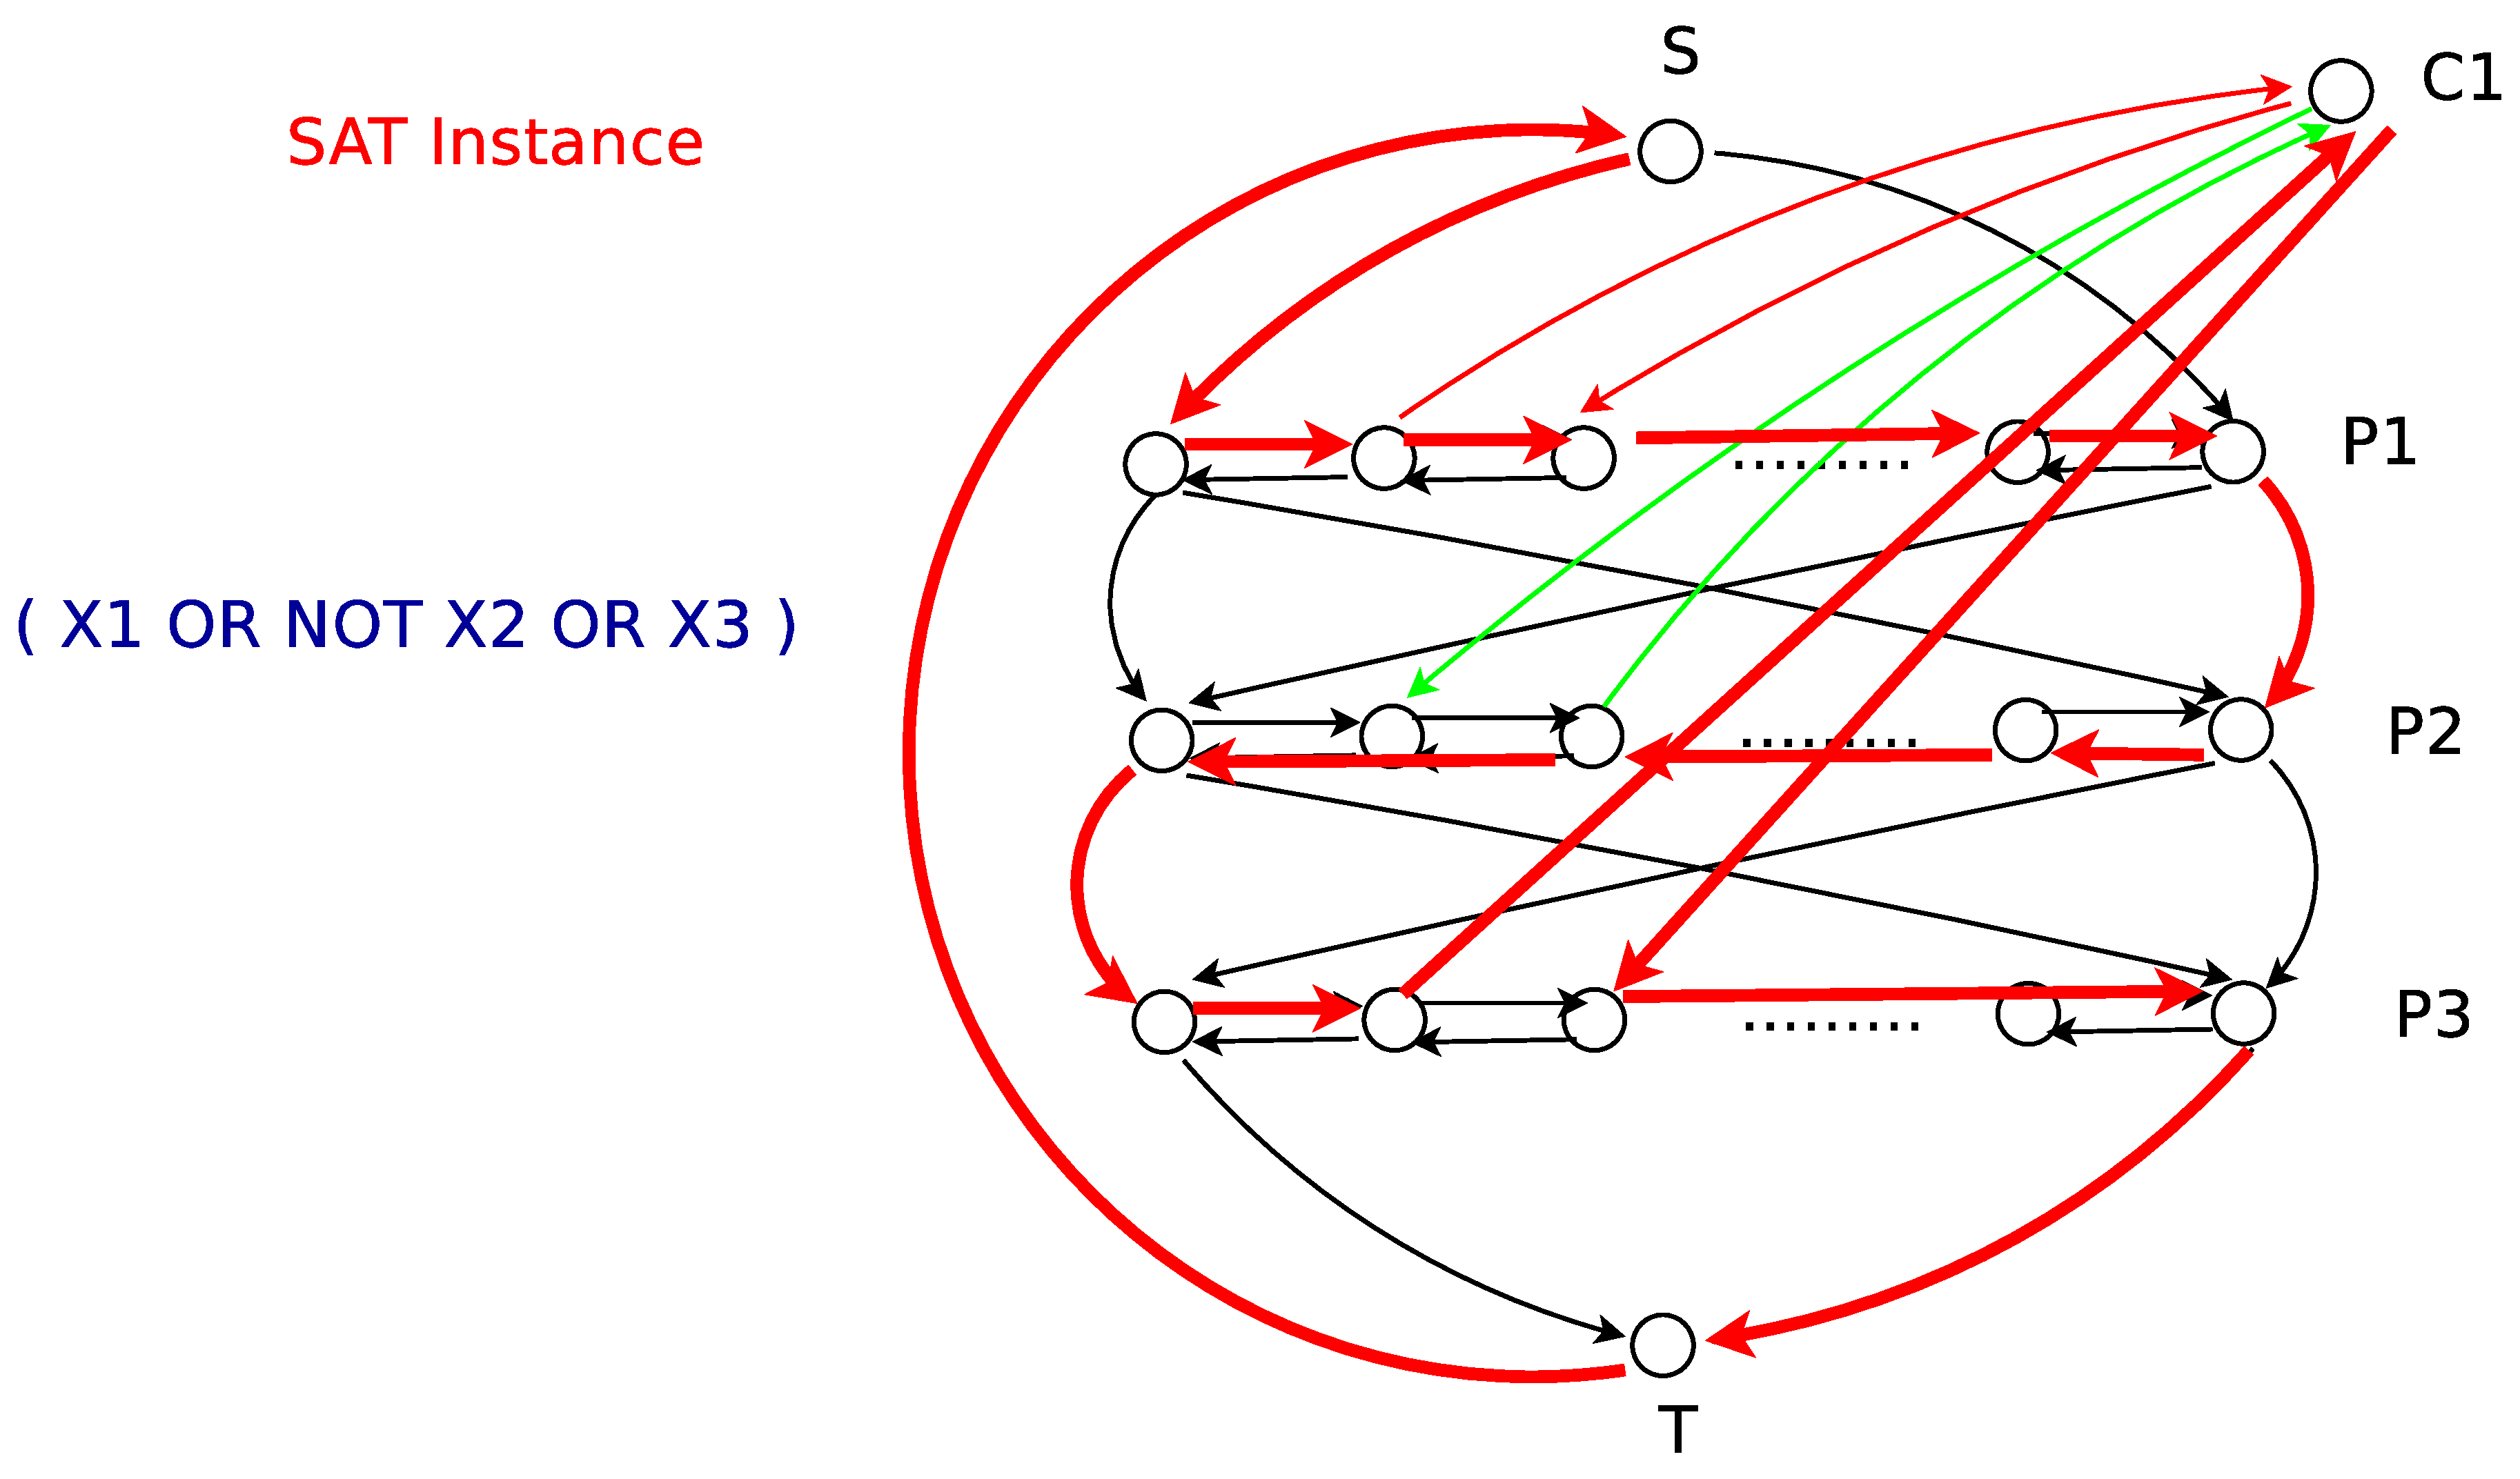
\includegraphics[width=3in]{L3-sathamilton-sat.eps}
\end{figure}

在图中,我们从节点$S$出发,因为$X_1 = \texttt{TRUE}$,所以第一排从左往右走,$X_2 = \texttt{FALSE}$,所以从第一排最右边节点直接到第二排最右边节点,然后从右往左走。$X_3 = \texttt{TRUE}$,所以从第二排最左边的节点直接到第三排最左边的节点,然后从左往右走。随后到节点$T$,最终回到节点$S$。不过我们注意到节点$C_1$并没有经过,所有点都经过了,只剩下$C_1$节点,怎么办呢?我们观察子句中哪个文字使得子句等于TRUE,$X_1$可以让子句等于TRUE,$X_3$可以让子句等于TURE,$X_2$也可以让子句等于TRUE,我们可以如图中选择的路径一样,从第三排进入节点$C_1$然后再走到$S$即可。大家可能觉得这种路径的选择是顺理成章,比较显然,那么接下来我们看看FALSE赋值,你会发现并不显然。

这里我们选择相同的SAT问题实例,即$X_1$ OR NOT $X_2$ OR $X_3$,我们存在一种赋值,使得子句等于FALSE,我们会发现如果按照FALSE所代表的路径走,没有办法达到目标。我们令$X_1 = \texttt{FALSE}, X_2 = \texttt{TRUE}, X_3 = \texttt{FALSE}$,此时子句等于FALSE。

\begin{figure}[H]
\centering
 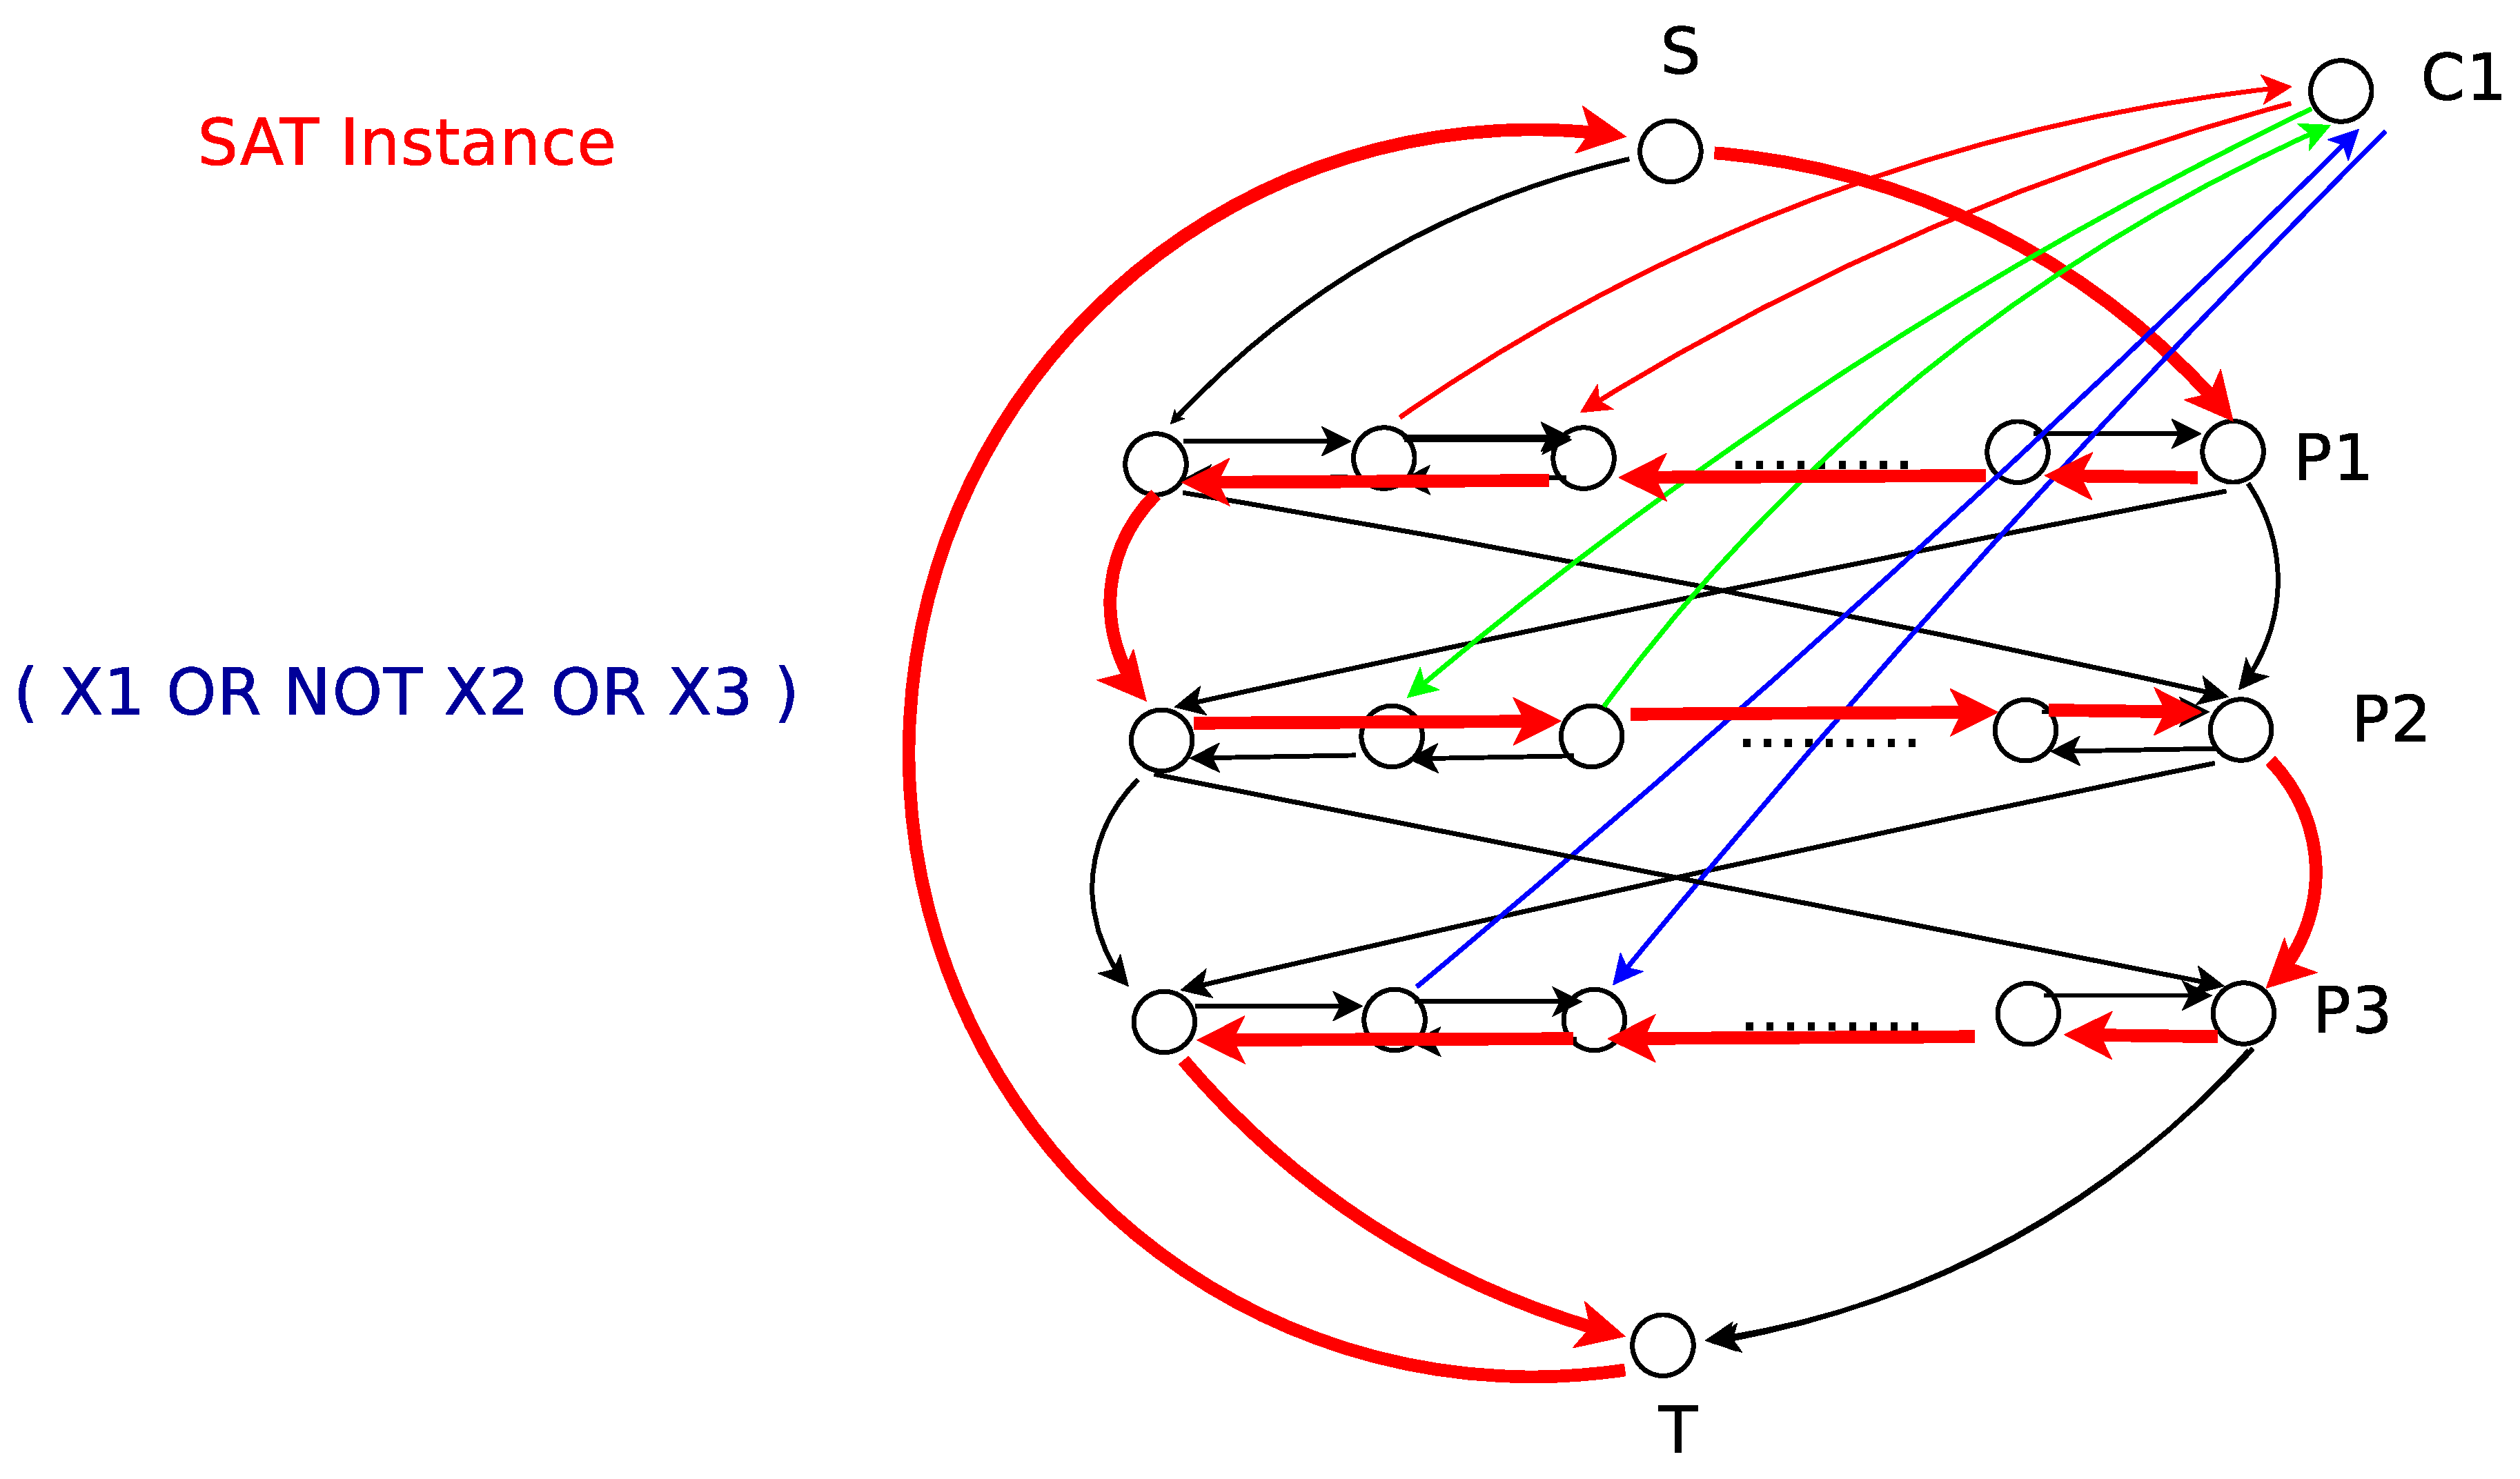
\includegraphics[width=3in]{L3-sathamilton-unsat.eps}
\end{figure}

现在我们按照TRUE和FALSE对应的方向在图中寻找路径,我们从$S$出发,因为$X_1 = \texttt{FALSE}$,所以第一排选择从右往左走,$X_2 = \texttt{TRUE}$,所以第二排选择从左往右走,第三排同理选择从右往左走,再到节点$T$,最后返回节点$S$,现在我们来观察一下有没有可能经过节点$C_1$,我们可以发现三排均不可能在限制条件下经过节点$C_1$,所以从这个例子中我们可以发现,一个FALSE的赋值没有办法在对应的图中找到一个满足限制条件(经过所有节点且每个节点只经过一次)的环路。

\subsubsection{归约——等价性}

看了刚才详细的剖析之后,我们就可以证明它们的等价性了,假如SAT问题的实例$\phi$是可满足的,也就是说我们能找到$X_i = \texttt{TRUE/FALSE}$的一种组合,使得子句的结果为TRUE,我们就从节点$S$出发,每一排如果是TRUE,则选择从左往右走,如果是FALSE,则选择从右往左走,从刚才的分析过程我们知道这样的路径肯定会经过每排的节点以及$S,T$节点。那么对于子句$C_j$,由于它是可满足的,所以至少有一个子句中的文字等于TRUE,则我们在相应的那一排肯定可以经过节点$C_j$。

\subsection{{\sc Hamilton Cycle} $\le_P$ {\sc TSP (Traveling Salesman Problem) }}
之前讲的归约属于比较复杂的归约过程,现在我们讲一个比较简单的归约,旅行商问题比哈密尔顿圈问题更难。旅行商问题我们第一节课就讲了,我们再看看这个例子是什么意思?

\subsubsection{旅行商问题(TSP)}

\begin{figure}[H]
\centering
 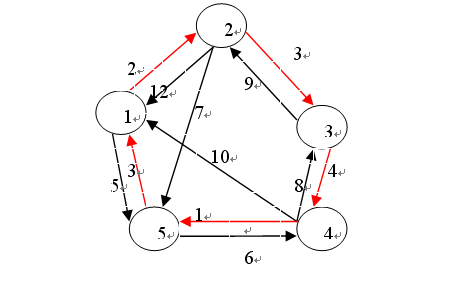
\includegraphics[width=3in] {tsp1.png}
\end{figure}


我们有五个城市,城市之间有道路,经过道路所花费的时间都有,例如1号和2号城市需要2小时,2号到1号需要12小时,等等。问题是说,这个商人能否从1号城市出发,经过所有的城市且每个城市只经过一次,再回到1号城市,并且花费的时间最短。这是一个优化问题,使得我们花费的时间最短,对于上图所示的例子,是沿着红色的路径($1, \ 2, \ 3, \ 4, \ 5, \ 1$)走花费的时间最短,可能存在其他的路径,但是花费的时间都会长于红色方案。

如今TSP问题被人们广泛研究,因为它在实际生活中用途广泛,在很久以前。Dantzig(线性规划), Fulkerson(网络流), 和 Johnson(《计算机与难解性》作者)都研究过这个问题。他们在1954年对美国的49个州的首府所抽象出来的问题,找到了最短路径,其抽象问题及其结果如下图所示。

\begin{figure}[H]
\centering
 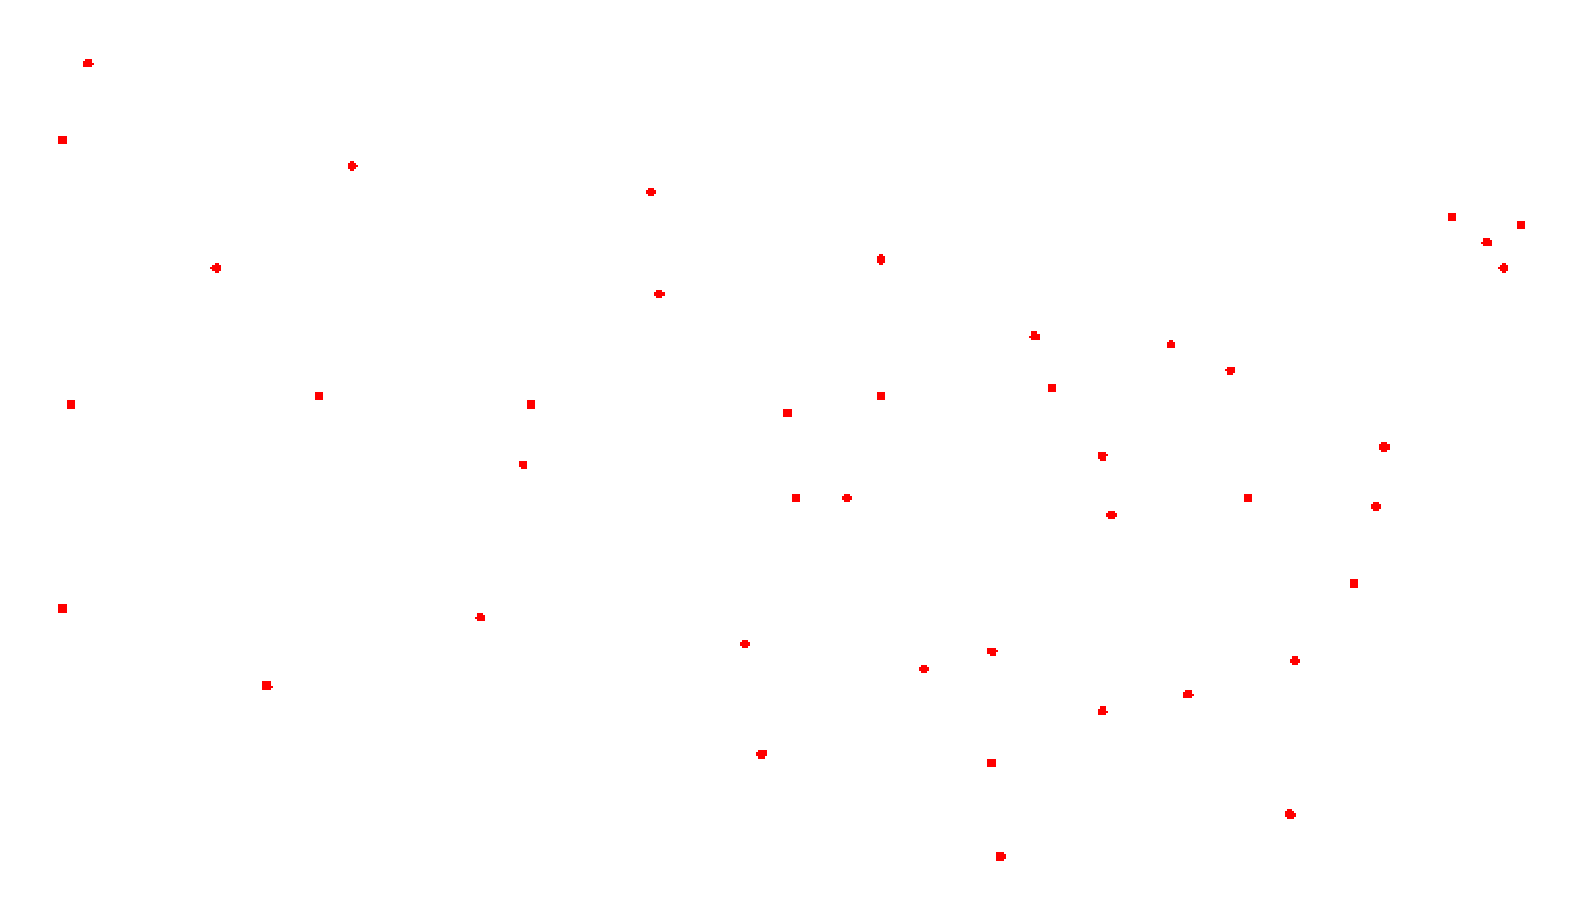
\includegraphics[width=1.8in] {L3-TSP42cities-map.eps}
\end{figure}

\begin{figure}[H]
\centering
 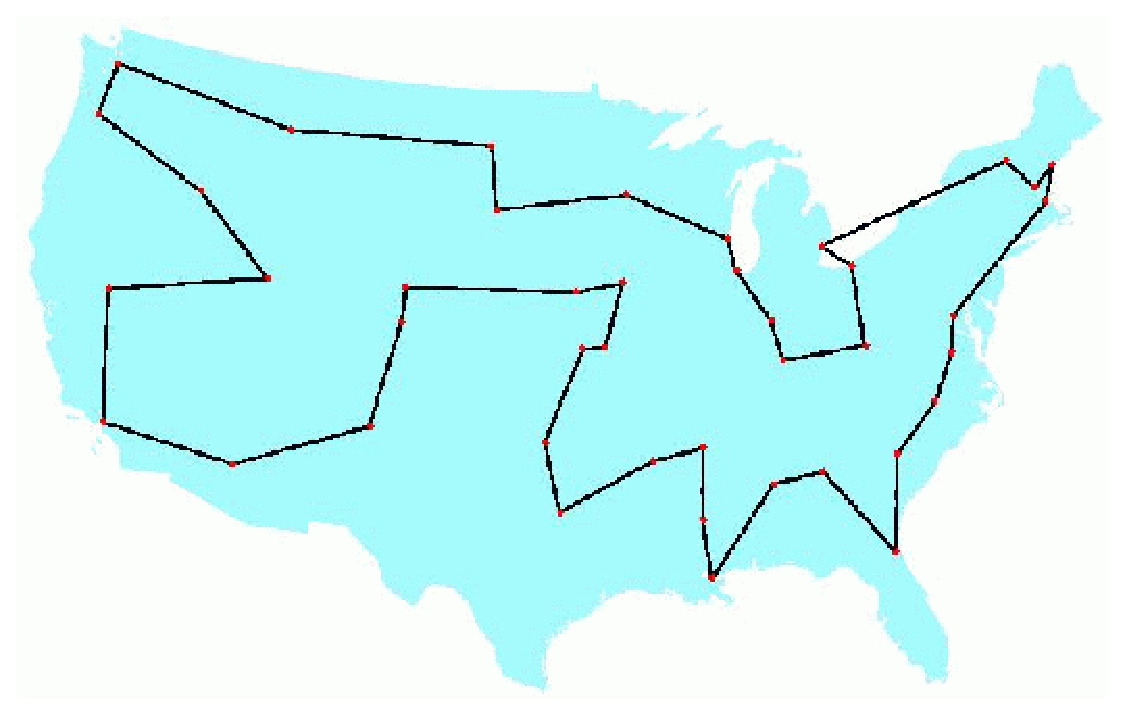
\includegraphics[width=1.8in] {L3-TSP42cities.eps}
\end{figure}

大家知道他们是怎么解决这个问题的吗?他们在每个节点上钉上一颗图钉,找一些细绳,在图钉之间进行缠绕,最后找到一条最短的路径出来。这个问题得到非常非常多的研究,我们可以从下图中了解这个问题的研究进展。

\begin{figure}[H]
\centering
 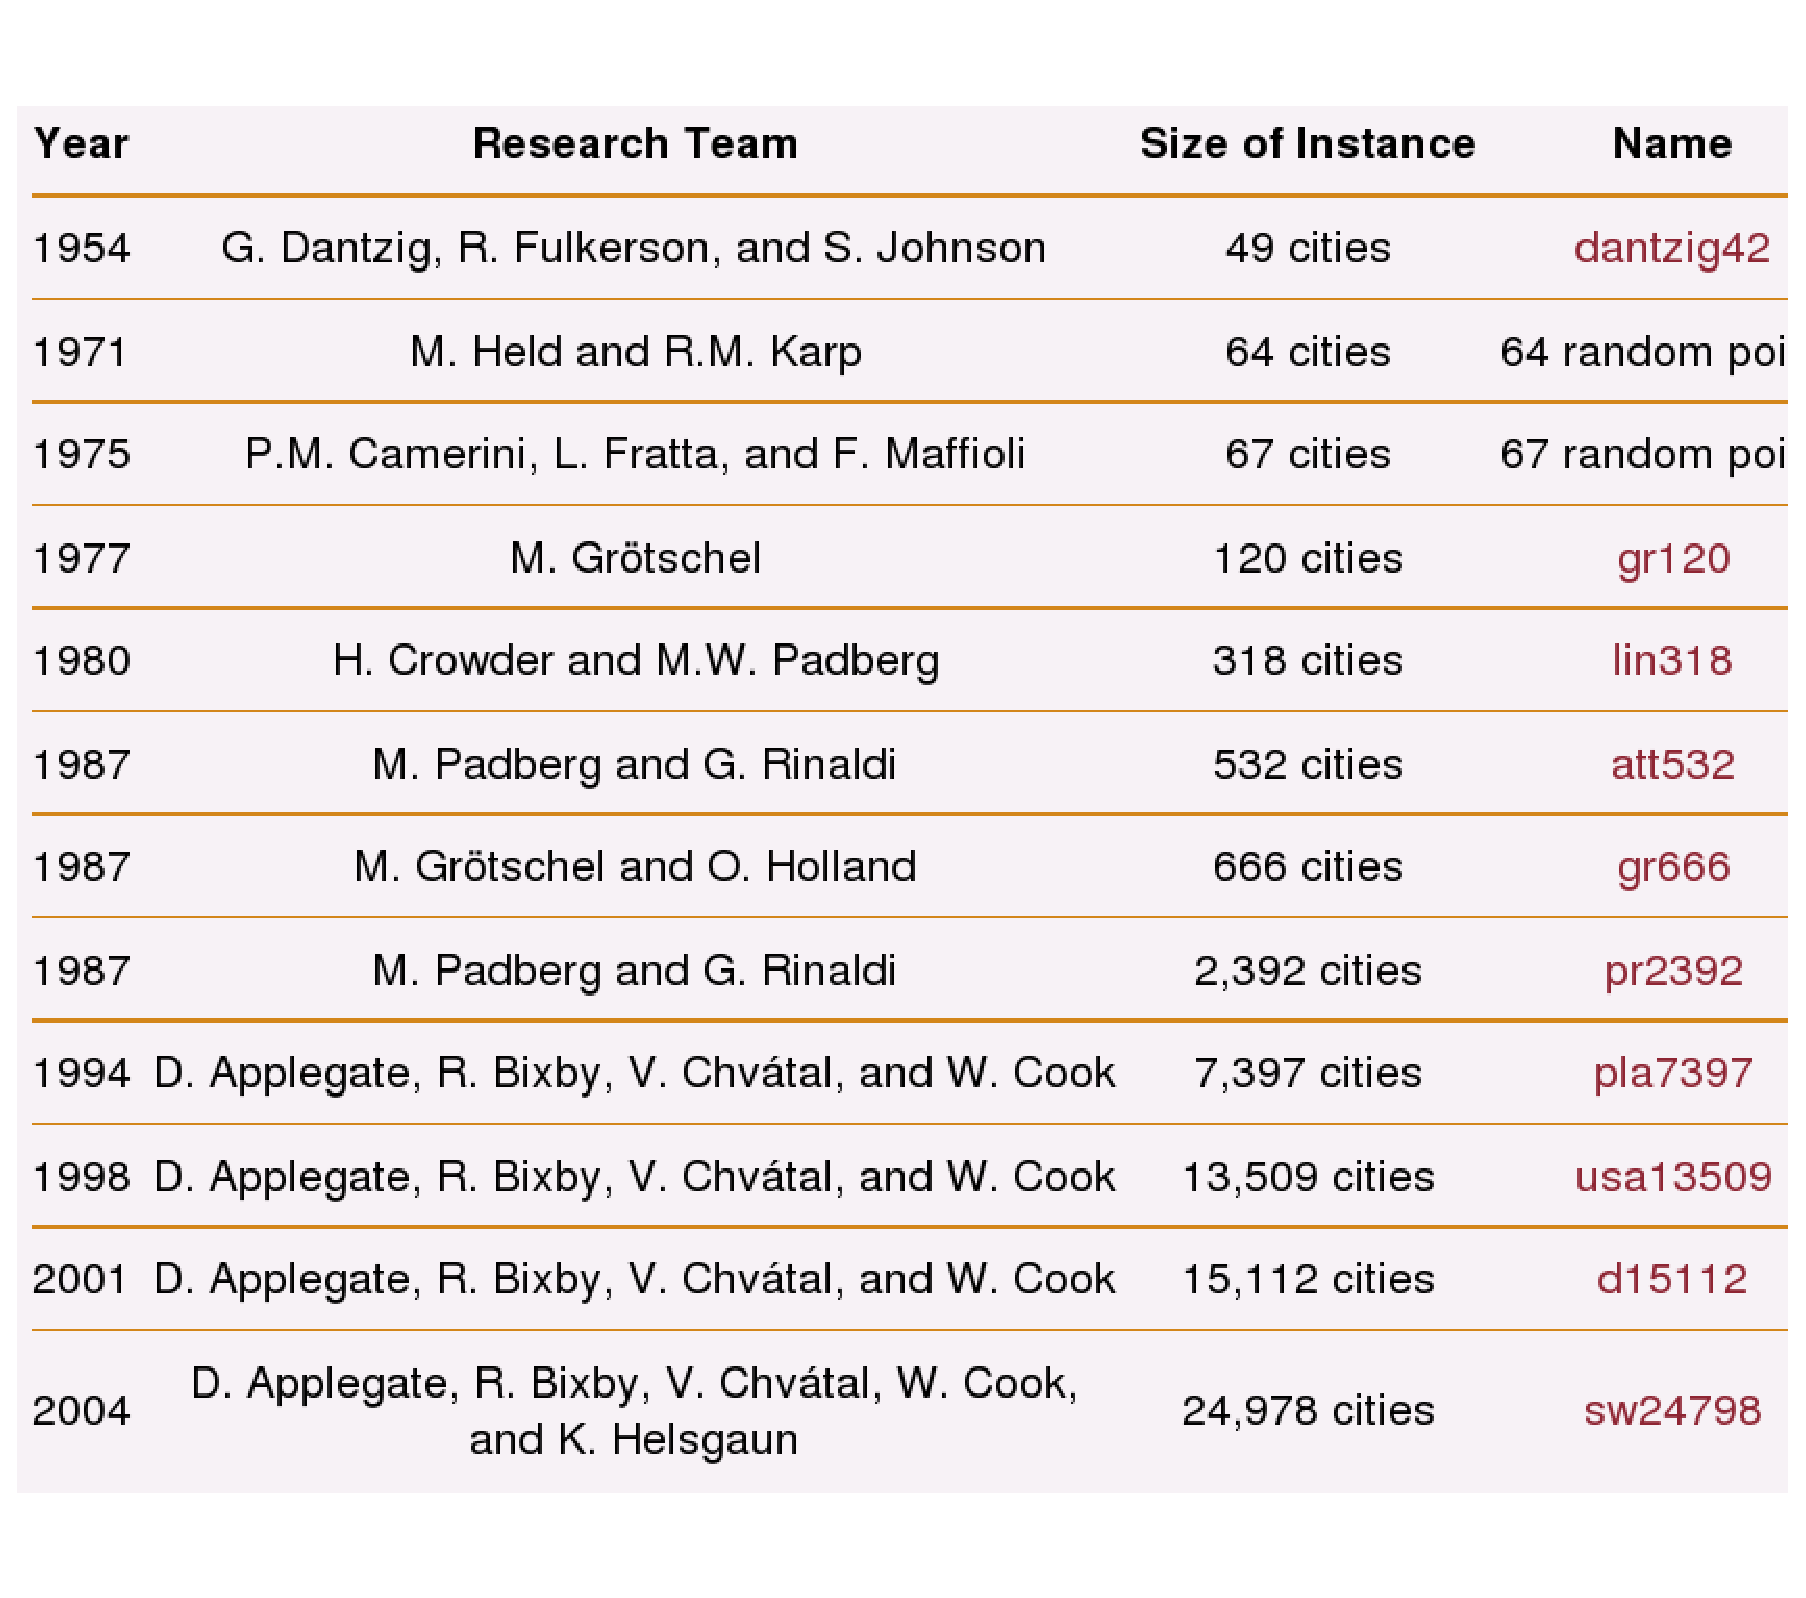
\includegraphics[width=2.8in] {L3-TSPprogress.eps}
\end{figure}

(引用自 http://www.tsp.gatech.edu/history/milestone.html.)


从中我们可以看到有许多著名专家学者孜孜不倦的寻找更优的答案,到现在为止能够解决24000多个城市。接下来我们看看旅行商问题的形式化定义。

 {\bf 输入:} 给定一个图 $G=<V,E>$, 距离 $d: E \rightarrow R$, 和一个界限 $B$; 

 {\bf 输出:} 是否存在一个哈密尔顿圈使得路径总长度小于等于 $B$?

 在这里稍微提示一下,原先是一个优化问题,为转换成判定问题,我们增加了一个参数(阈值)B。

 \subsubsection{归约——变换,等价性}

 为什么我们说TSP问题比哈密尔顿圈问题更难呢?因为任何一个哈密尔顿圈问题我们都能转换成一个TSP问题。给我们一幅左图,哈密尔顿圈问题是是问这个里面存不存在一个环路,相应的我们构造一个如右图所示的旅行商问题。

 \begin{figure}[H]
 \centering
 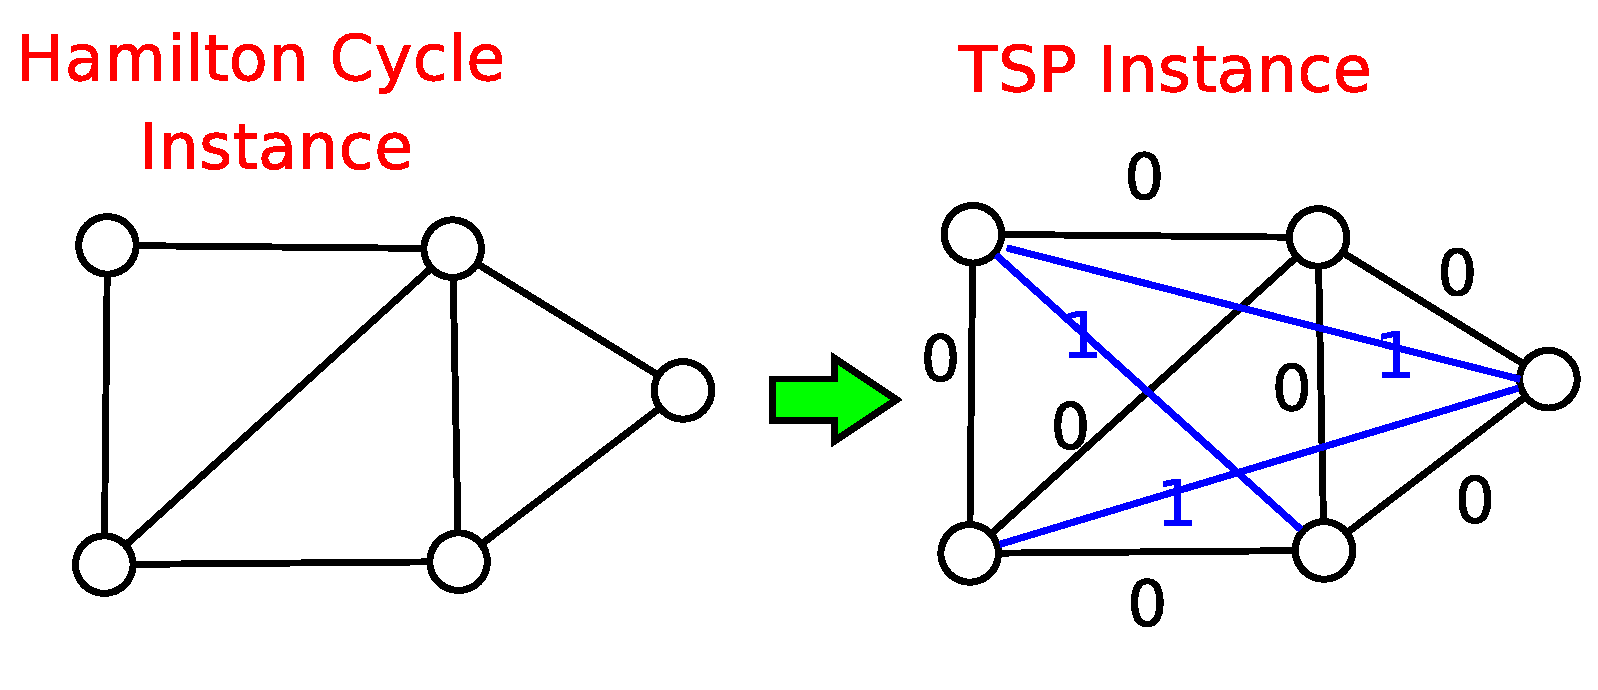
\includegraphics[width=3in] {L3-hamiltoncycletsp.eps}
\end{figure}

我们把节点之间所有可能的连接都画出来,原先的边距离都是0,新添加的边距离都是1,问在右图中能否旅行所有的城市且每个城市只经过一次,回到原点且总里程数小于等于0。很明显啊,在右图中是存在一条满足要求的环路(沿着左图中外围的边走一次即可)。所以这一下就证明了,旅行商问题比哈密尔顿圈问题要难,因为旅行商问题很容易就转换成哈密尔顿圈问题。左图存在一个环路,则右图就存在一条路径总里程小于等于0。

\subsubsection{扩展阅读:使用DNA计算机计算哈密尔顿圈问题}

现在我们知道旅行商问题和哈密尔顿圈问题都很难,用电子计算机很难求解,因此大家就考虑能否使用DNA计算机进行快速求解。

在这里给大家补充一点重要知识,在1994年的时候,Leonard M. Adleman发明了世界上第一台DNA计算机,这台计算机就能求解哈密尔顿圈问题。Leonard M. Adleman同时也是RSA加密算法的发明者之一,而这两项工作也是他最著名的工作。

\begin{figure}[H]
\centering
 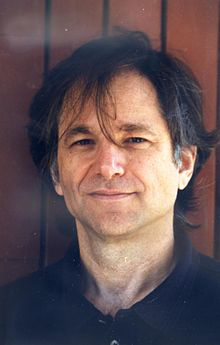
\includegraphics[width=0.8in] {Adleman.png}
\end{figure}

他在《科学美国人》杂志上曾撰写一篇文章,来讲述他发明DNA计算机的过程,他用分子机制来求解哈密尔顿圈问题,我们来看看他这个东西是怎么做的。

我们给出一个哈密尔顿圈的实例。

\begin{figure}[H]
\centering
 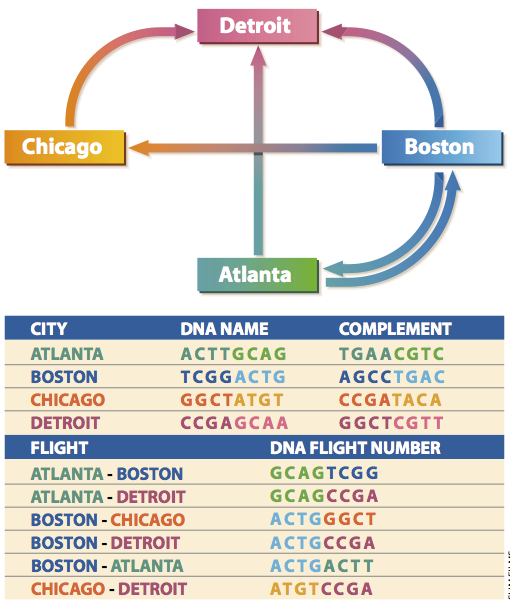
\includegraphics[width=2.8in] {DNAComputer1.png}
\end{figure}

图中有芝加哥,底特律,波士顿和亚特兰大四个城市,城市之间的航班如图中所示,现在我们需要旅行所有城市且每个城市只经过一次。并且我们降低难度,不需要形成环路,而只需要旅行所有城市且每个城市只经过一次即可,大家想想怎么旅行。唯一一条满足要求的路径为亚特兰大——波士顿——芝加哥——底特律。现在我们用DNA计算机来求解这个问题,DNA计算机是怎么构造的呢?

每个城市都随机合成了一小段8碱基DNA,同时合成它的互补链,以亚特兰大为例,合成的8碱基DNA链为$-ACTTGCAG-$,则其互补链为$-TGAACGTC-$。对于8碱基的DNA链,我们分成前4个碱基和后4个碱基。对于图中的每个航班我们也合成一段DNA,以亚特兰大到波士顿的航班为例,我们合成一段DNA$-GCAGTCGG-$,它是由亚特兰大的后4位碱基$-GCAG-$和波士顿前4位碱基$-TCGG-$连接而成,其他航班也类似的合成一段DNA。然后把这些合成的DNA放入试管中,加入DNA聚合酶,此时我们就可以解决了哈密尔顿圈问题。

\begin{figure}[H]
\centering
 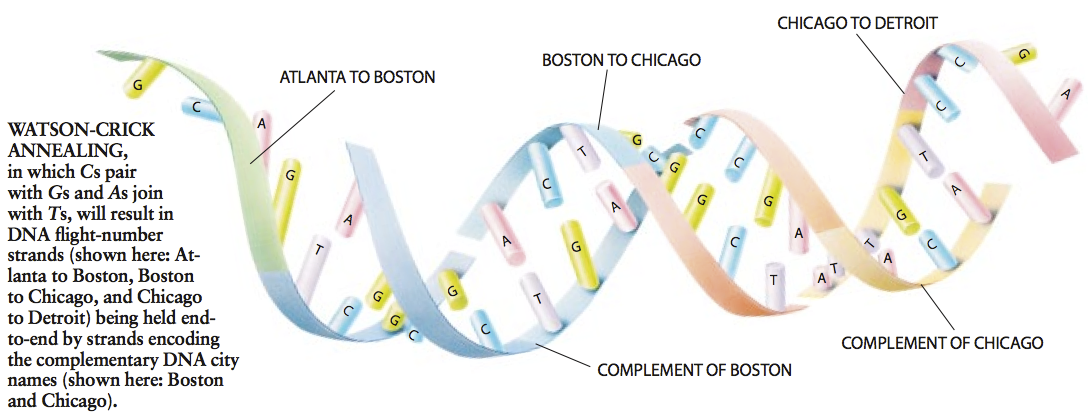
\includegraphics[width=4.5in] {DNAComputer2.png}
\end{figure}

从图中合成的DNA我们可以看到,前4位是亚特兰大的后4位,接着再是波士顿的前4位,由于存在互补DNA链,因此进行碱基互补配对后,波士顿的前4位碱基会和波士顿的后4位碱基进行连接,形成完整的代表波士顿的8位碱基DNA。而波士顿的后4位又和芝加哥的前4位连接到一起,如此这般,所有能够连接到一起的DNA片段都连接到了一起,而其中最长的DNA链就是我们的哈密尔顿路径,剩下的问题就是把这个最长的链找出来即可。

DNA计算机刚刚问世时,中国科学院计算技术研究所的老师们曾对DNA计算机技术进行过研究,认为DNA计算是一种专用计算机,且需要消耗大量的DNA,所以当时认为DNA计算机还不能进行大规模应用,而量子计算机更有可能投入应用。

\subsection{{\sc SAT} $\le_P$ {\sc Graph Coloring}}
下面我们再来讲一个证明,图着色问题比SAT问题更难。为什么我们一直在讨论比逻辑问题,可满足性问题要难的问题呢?因为到最后我们要证明逻辑问题比所有问题都要难,它是最难最难的问题,换句话说它比其他问题都要难,所以大家的难度系数是一样的。下堂课我们将介绍为什么一直在讨论SAT问题。

\subsubsection{图着色问题}

我们先看一个可抽象成图着色问题的实际问题——室内定位。室内定位现在主要依靠Wifi,假设现在有n个Wifi,每个Wifi都有好几个波段,如果两个Wifi离的很近的话,则两个Wifi不能用同一个波段,否则就会产生干扰。现在问题就很清晰了,假设有n个Wifi,Wifi信号源的地理位置已知,我们应该怎么安排每个Wifi信号源的波段,使得相互之间不会发生干扰现象。我们总共可用的波段很少,比如每个Wifi只有K个波段可以使用,我们应该怎么设计?我们把上面描述的实际问题抽象成一个数学问题。

 {\bf 输入:} 一个图 $G=<V,E>$, 一个整数 $k$; 

 {\bf 输出:} 是否存在图$G$的 $k-着色$ 使得每个节点都有一个颜色, 但任何一条边的两个端点颜色不同?

 我们举个例子来说明一下。

\begin{figure}[H]
\centering
 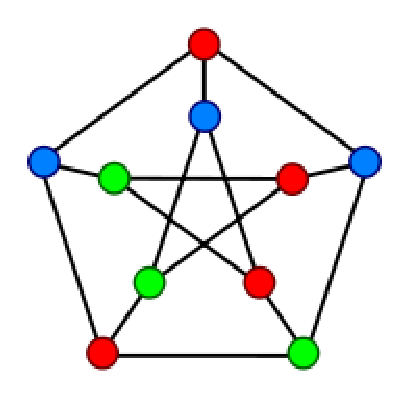
\includegraphics[width=1.5in] {180px-Petersen_graph_3-coloring.eps}
\end{figure} 

这个图叫Petersen图,外面是个五边形,里面是一个五角星,对应的节点进行连接形成一个Petersen图。我们问能否进行3着色?这里如果将每种颜色想象成一个波段,就类似于我们上面讲的实际例子了,所以这是一个很有用的问题。这个例子可以进行3着色,按图所示的方式进行着色,可以保证任何一条边的两个端点颜色都不相同。

\subsubsection{图着色问题分类及其关系}
图着色问题有很多种类,刚才我们提到的例子是顶点着色,也就是说每个顶点我们给一个颜色,使得相邻的顶点颜色不同。类似的还有边着色问题,我们能否对边进行着色,使得任何相邻的边都没有相同的颜色。我们最熟悉的是第三类问题,称为面着色问题,著名的四色地图就是说对于美国地图,相邻的州着不一样的颜色,所以称为面着色问题,当然对于地图的形式还是有一些要求。这三类问题我们用图说明。

\begin{figure}[H]
\centering
 \begin{minipage}{0.3\textwidth}
 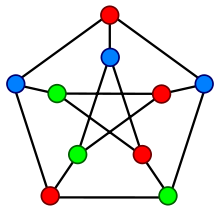
\includegraphics[width=\textwidth]{L3-vertexcoloring.png}
 \caption{  Peterson graph  }
\end{minipage}
\begin{minipage}{0.3\textwidth}
 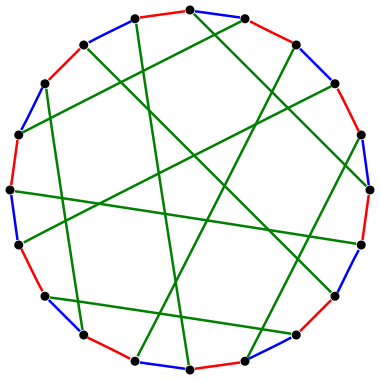
\includegraphics[width=\textwidth]{L3-edgecoloring.png}
 \caption{ Desargues graph: the complement of Peterson graph }
\end{minipage}
\begin{minipage}{0.3\textwidth}
 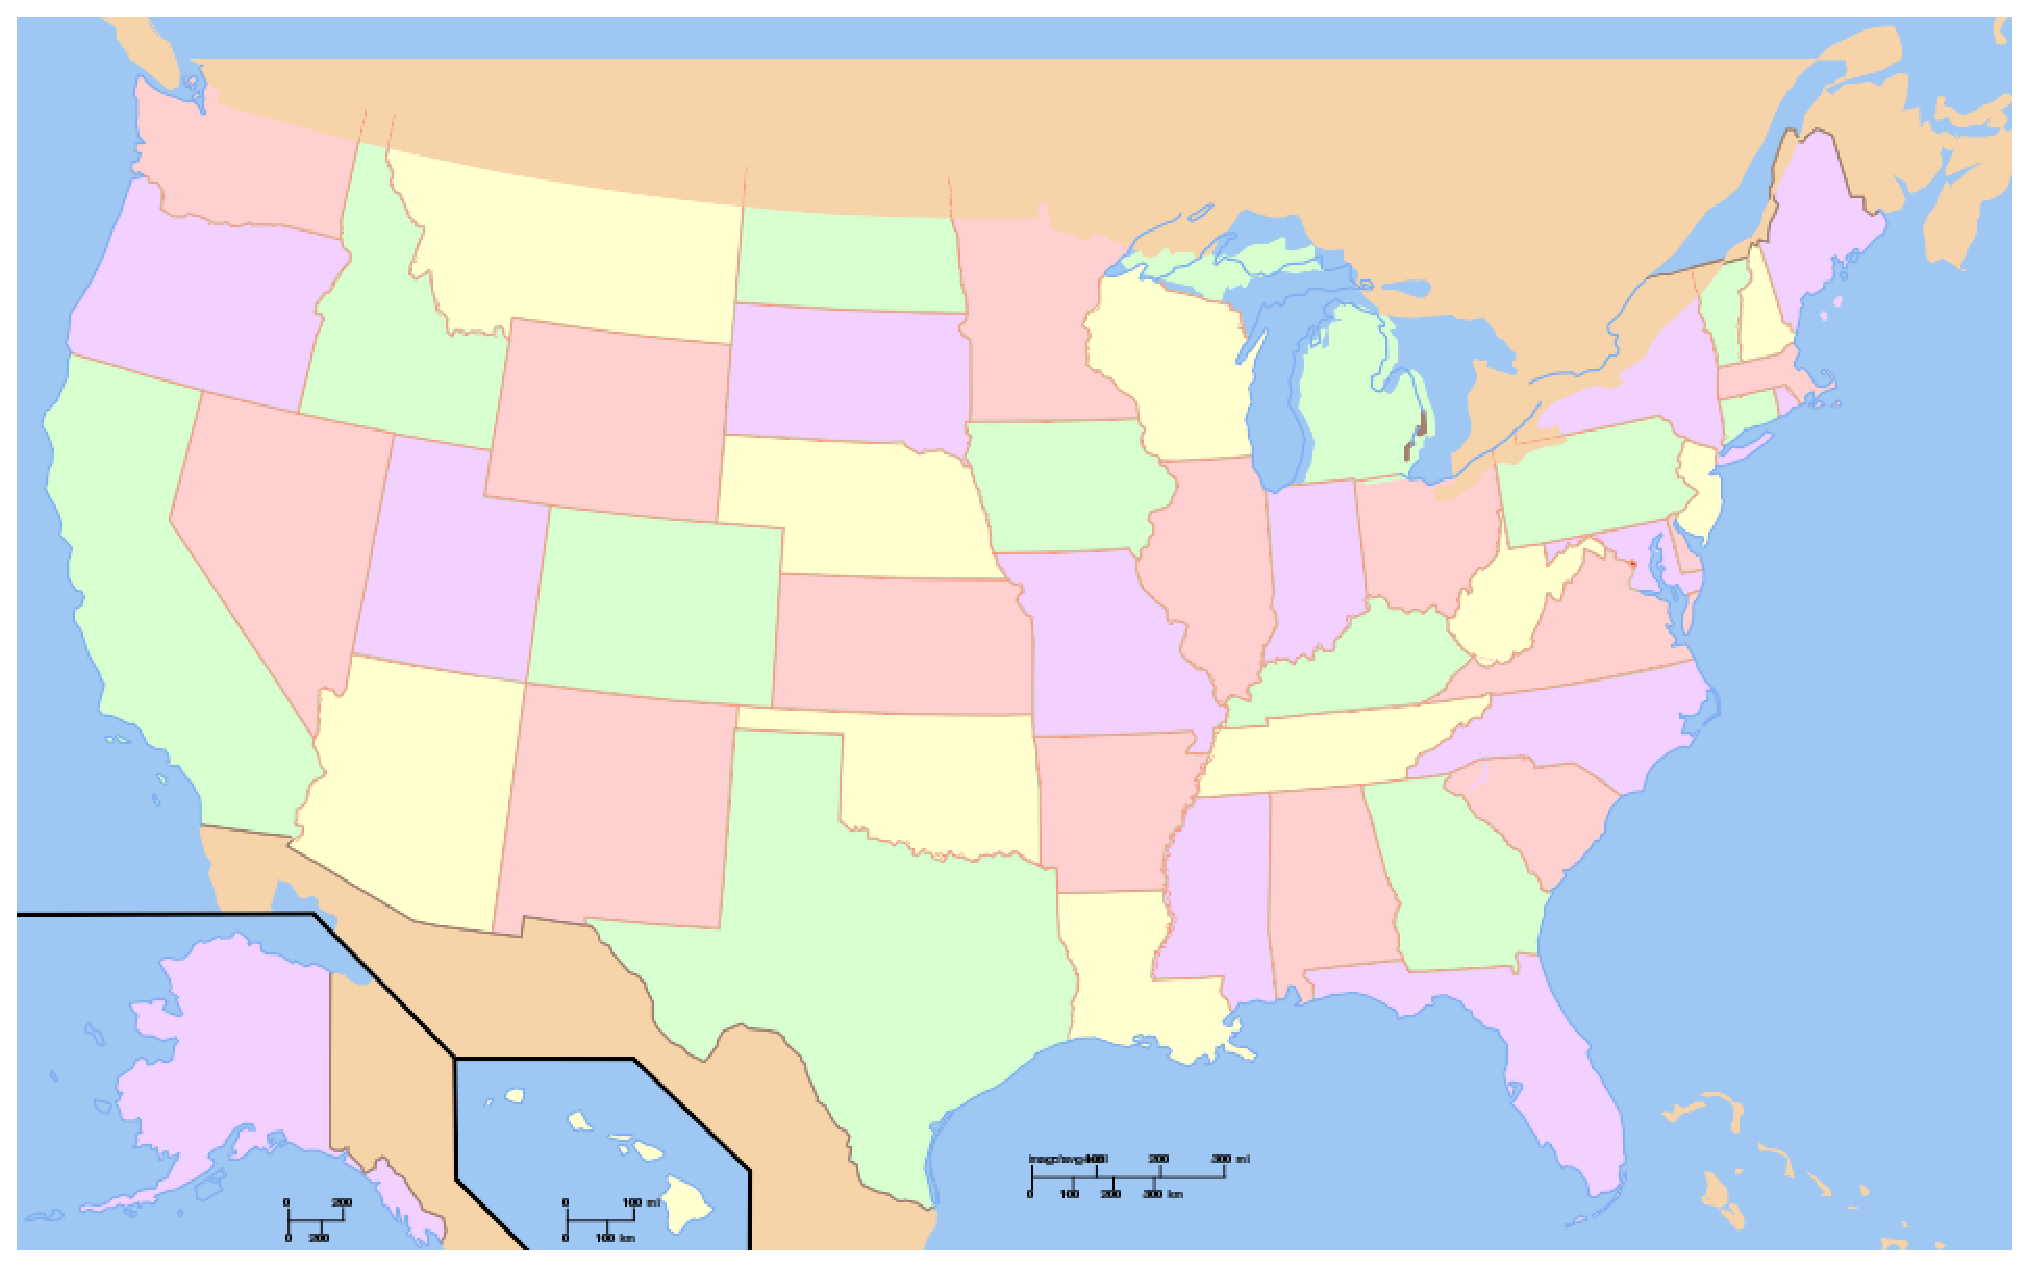
\includegraphics[width=\textwidth]{L3-facecoloring.eps}
 \caption{  USA map }
\end{minipage}
\end{figure}

我们说这三类问题中,第一个顶点着色问题是最本质的,边着色和面着色问题都可以归结为第一个顶点着色问题,所以我们只需要研究顶点着色问题即可。

那么为什么边着色问题可以归结为顶点着色问题呢?假如我们需要对左图进行边着色,则任意相邻的边不能有相同的颜色,我们把它转换成顶点问题,我们对每条边单独做一个顶点,然后相邻的边所代表的顶点之间连接一条边,所以对左图进行边着色就等价于对右图中的绿色的顶点进行顶点着色。

\begin{figure}[H]
\centering
 \begin{minipage}{0.4\textwidth}
 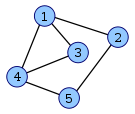
\includegraphics[width=\textwidth]{L3-linegraph1.png} 
 \end{minipage}
 \begin{minipage}{0.4\textwidth}
 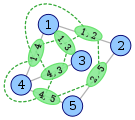
\includegraphics[width=\textwidth]{L3-linegraph2.png} 
 \end{minipage}
\end{figure}

面着色也是同样的,假设下图蓝色部分表示一幅地图,我们需要对左,中,右,以及外面进行着色,使得四个面的颜色不相同。

\begin{figure}[H]
\centering
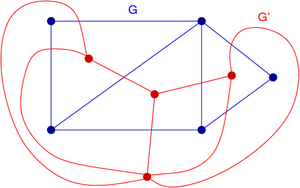
\includegraphics[width=2in]{L3-dualgraph.png} 
\end{figure}

我们也能转换成顶点的问题。我们构造一个新的图,每个面是一个顶点,两个顶点之间有边相连,所以总共有四个顶点,七条边。所以对蓝色的地图进行面着色等价于对外面红色图进行顶点着色。所以顶点着色是最本质的。

接下来我们看一个顶点着色最简单的例子,给我们一幅图,能否进行2着色?这种特殊的情况是很快就可以解决的,没有什么难度。因为这幅图一旦用两种颜色着色,这幅图肯定是一幅二部图,以下图为例。

\begin{figure}[H]
\centering
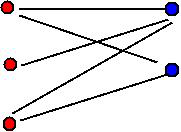
\includegraphics[width=1in]{L3-2coloring.png} 
\end{figure}

我们把红色的放左边,蓝色的放右边,相同的颜色的顶点之间没有边连接,所以边都在红色节点和蓝色节点之间,所以它肯定是一个二部图。判定一个图是否为二部图很简单,运行广度优先搜索即可。

我们先粗略的看一下进展,判定一个图2着色是很容易的,那么判定k着色呢?一幅图我们可以使用动态规划的方法,因为一幅图还是可以进行分割的,但是这个动态规划方法很慢,时间复杂度为$O(2.445^n)$,是指数级的运算时间。后来又使用了一些办法使得k着色问题的算法时间复杂度降低为$O(2^nn)$,还是指数级。对于三着色或四着色,有一些比较好的进展,时间复杂度降低为$O(1.3289^n)$和$O(1.7504^n)$,还是指数级的时间复杂度。以上就是图着色问题的最新进展,大家可以看出图着色问题很难,因为到现在为止设计的所有算法都是指数级的算法。下面我们来说明图着色问题比SAT问题更难。

\subsubsection{归约——构造三角形、分叉结构}

为什么说图着色问题比SAT问题更难?我们还是要设计一些精巧的东西,它能模拟SAT问题中的逻辑关系。我们还是先对图着色问题画一些小的例子,发现三角形很特殊,假如我们画一个三角形,然后对它进行3着色,我们用图形表示如下。

\begin{figure}[H]
\centering
 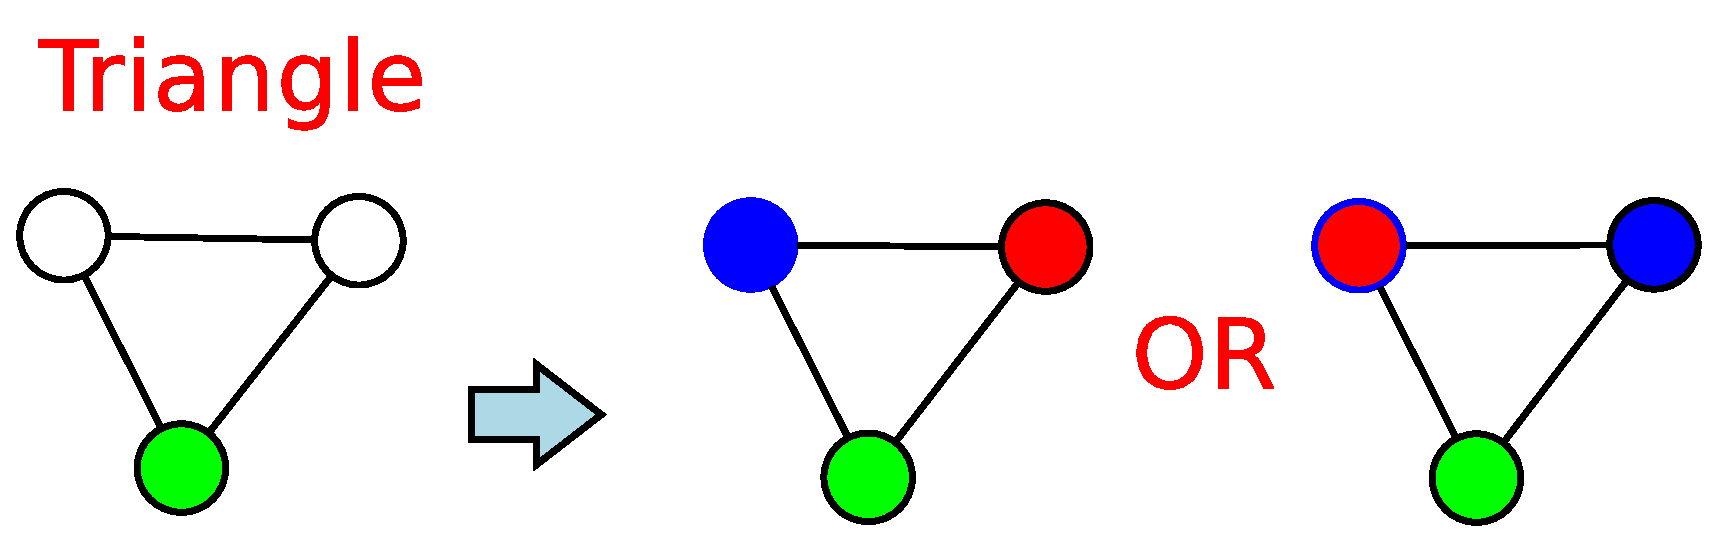
\includegraphics[width=3in] {L3-coloringgadgettriangle.eps}
\end{figure}

不妨假设底部的节点为绿色,那么顶部的两个节点不能为绿色,要么是红色,要么是蓝色,所以要么左边节点为红色,右边节点为蓝色;要么左边节点为蓝色,则右边节点必须为红色,两种情形均已表现在上图中。大家可能注意到,在上述描述中仍然蕴含着逻辑或关系,即我们可以用这两种情况模拟SAT问题中的\texttt{TRUE or FALSE},我们不妨设左边的情形为FALSE,右边的情形为TRUE。这样我们就可以考虑用这个来模拟SAT问题中的或关系(or),$X_i = \texttt{TRUE/FALSE}$。所以我们需要观察一些小的例子,这些例子当中有些特性和其他问题的特性很像,这样我们能用一些小的例子来模拟这些特性,在这个例子中我们可以模拟或关系(or)。

我们再来尝试构造另外一个精巧的东西,一个类似于叉子的树状结构,它分为三个分叉。

\begin{figure}[H]
\centering
 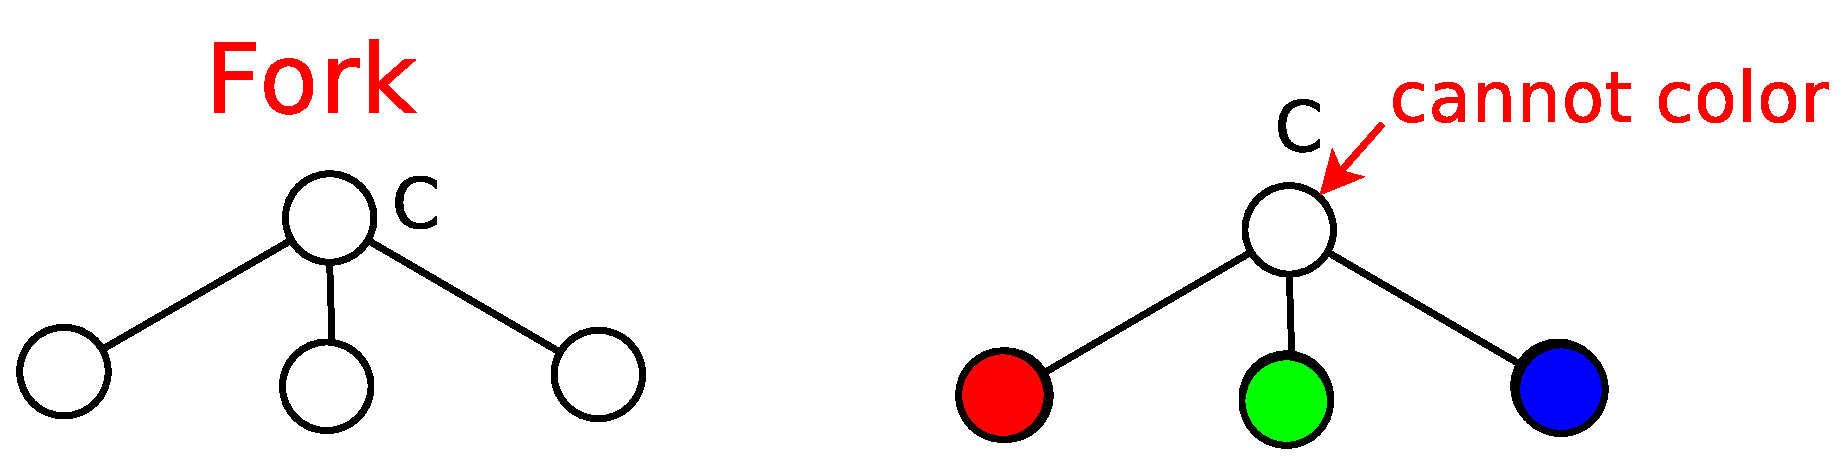
\includegraphics[width=3in] {L3-coloringgadgetfork.eps}
\end{figure}

给我们如上图所示的图进行着色,则下面点不能把三种颜色都用尽。假如下面三个节点的颜色为红,绿,蓝,这个怎么着色呢?所以如果想对图进行着色,则下面三个节点只能用两种颜色,一种也可以。

\subsubsection{归约——构造组合“王冠”}
把上面讲的两个例子组合到一块,又构成了一个稀奇古怪的东西,一个王冠。

\begin{figure}[H]
\centering
 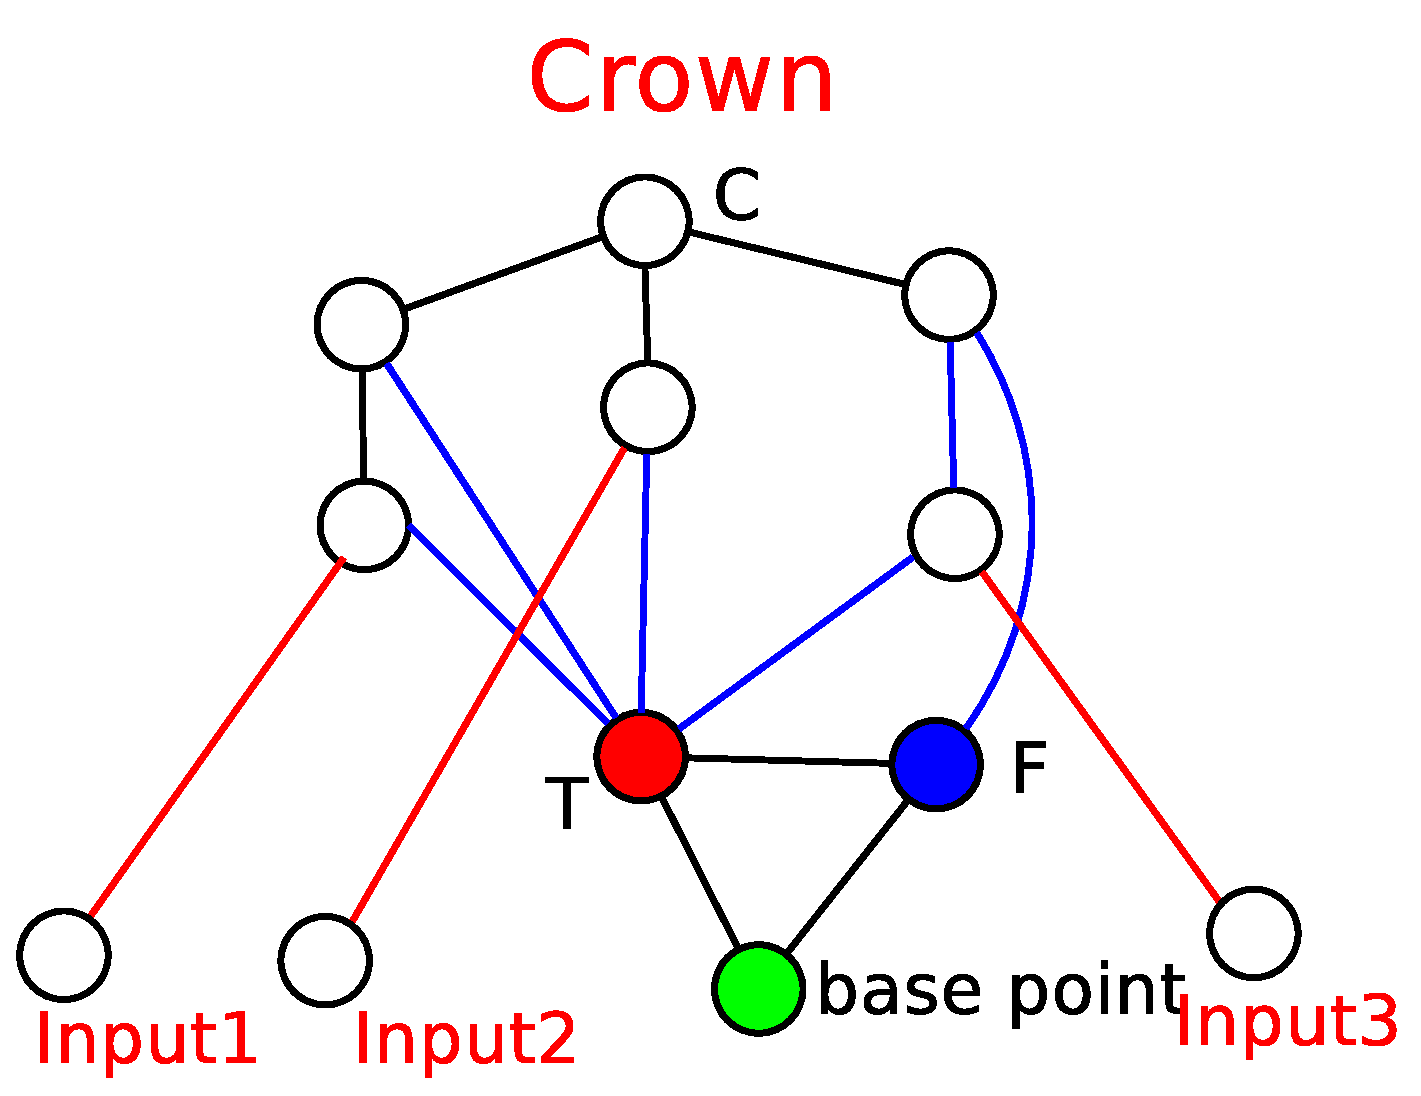
\includegraphics[width=2in] {L3-coloringgadgetcrown.eps}
\end{figure}

大家注意,在这里可能提前要给大家说一下,我们在证明一个问题比另外一个问题难的时候,我们找的都是稀奇古怪的情况,都是精心设计的图。这里也是精心设计的王冠,上面一部分是顶部一个点,下面分成3个叉,3个叉分别垂下来一个节点,底部我们先画好一个三角形,这个三角形当作基准放在这里,因为这个三角形三个顶点分别着三种颜色,所以作为一个基准放在这里。这种设计的确是很古怪的设计,但是也是很巧妙的一种设计。接下来我们看看精巧的地方在哪里。

第一种情况,我们对三个INPUT均赋值BLUE,则我们会发现没有办法对节点$C$进行着色。

\begin{figure}[H]
\centering
 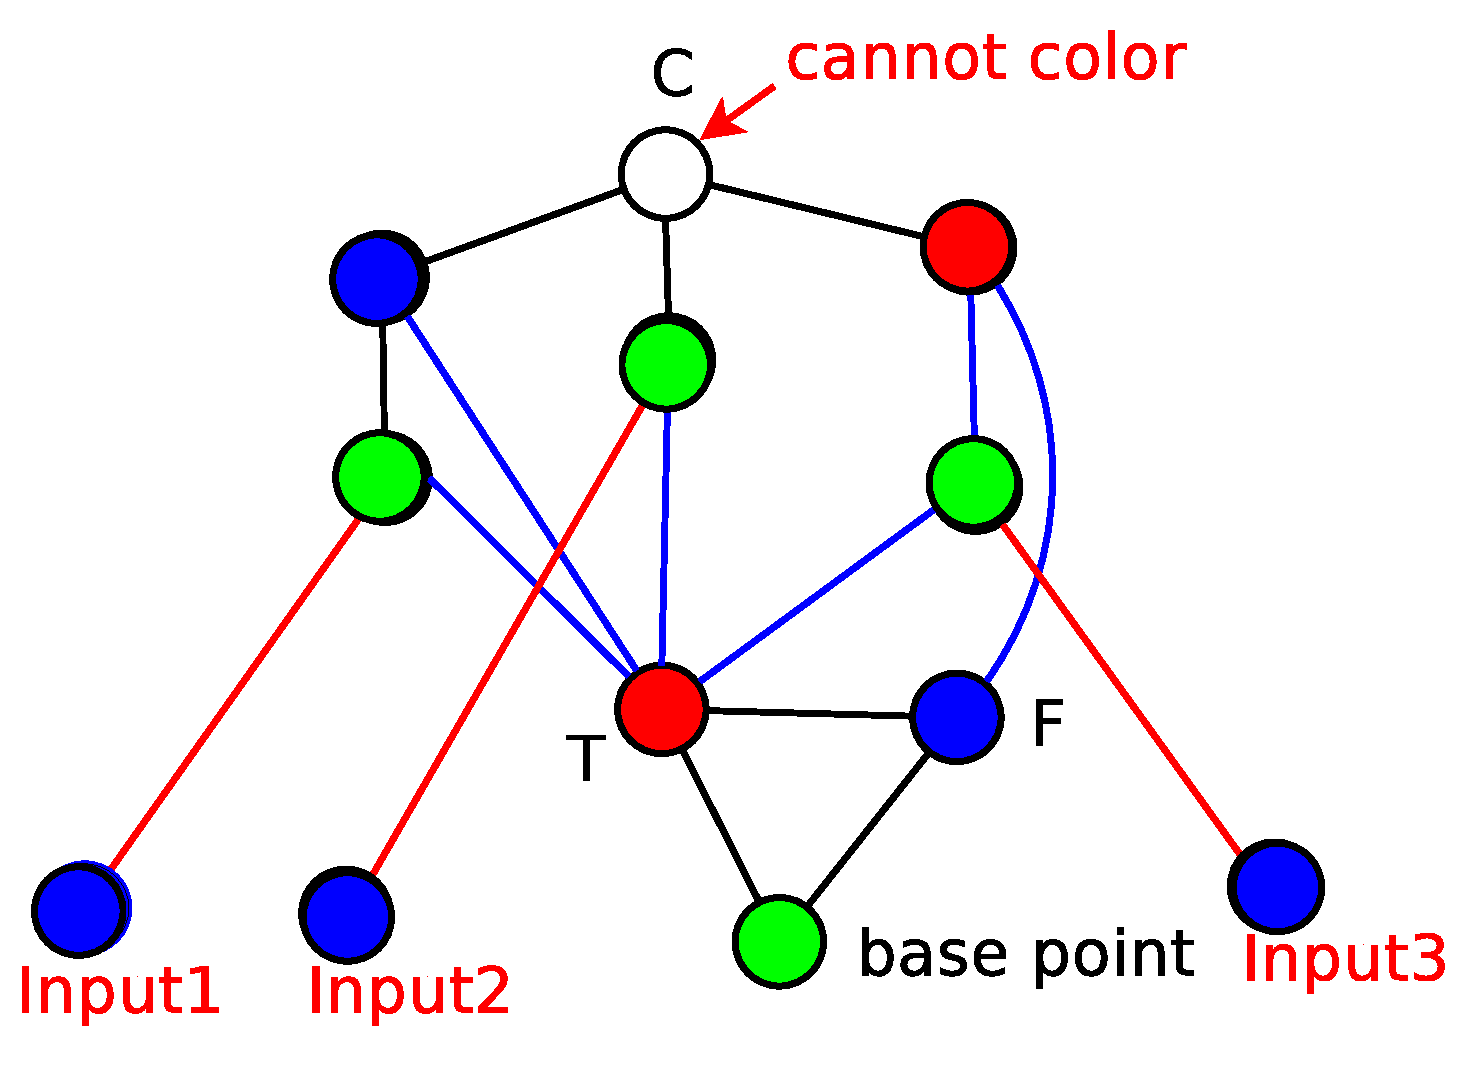
\includegraphics[width=2in] {L3-coloringclausecrownBBB.eps}
\end{figure}

即如果三个输入均为FALSE,则顶部节点没有办法进行着色,接下来我们详细分析一下。在这幅图中三角形的颜色是固定的,然后导致分叉下面的三个节点必须为绿色,从而导致分叉的三个节点为红,蓝,绿三种颜色,所以节点$C$不能进行着色。所以我们可以得出结论,三个输入不能同时着蓝色,即SAT问题的$X_1,X_2,X_3$不能同时取FALSE,

第二种情况,假设我们三个输入的取值为蓝,蓝,红,则我们可以验证对节点$C$能够进行着色。

\begin{figure}[H]
\centering
 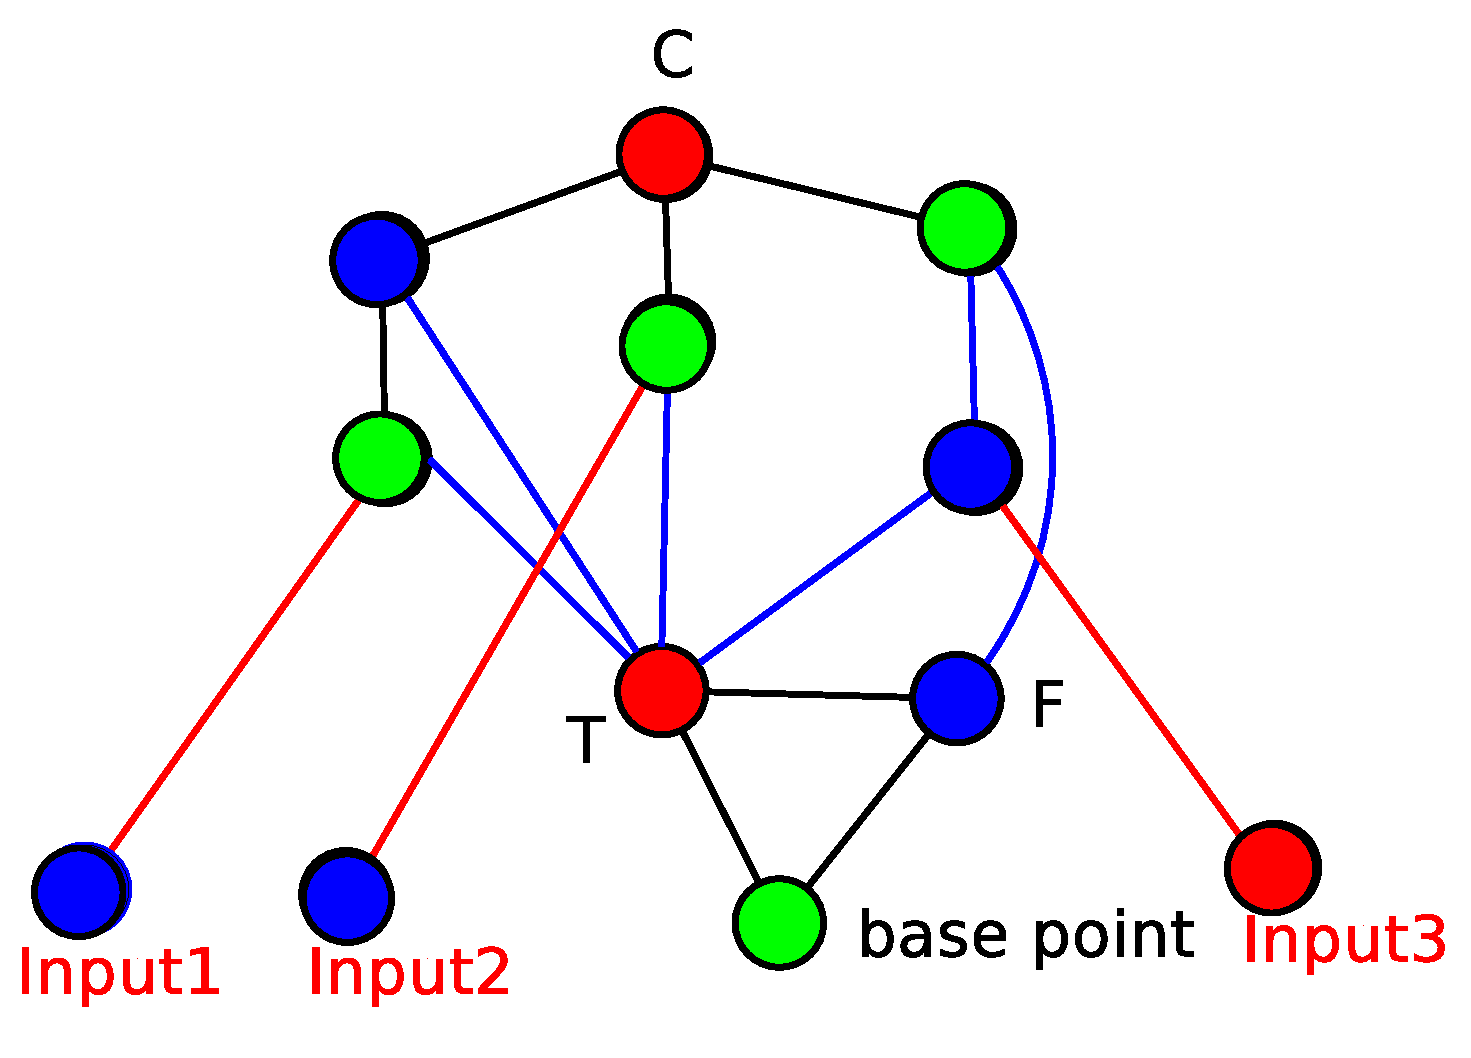
\includegraphics[width=2in] {L3-coloringclausecrownBBR.eps}
\end{figure}

第三种情况,假设我们三个输入的取值为蓝,红,蓝,我们同样可以验证对节点$C$能够进行着色。

\begin{figure}[H]
\centering
 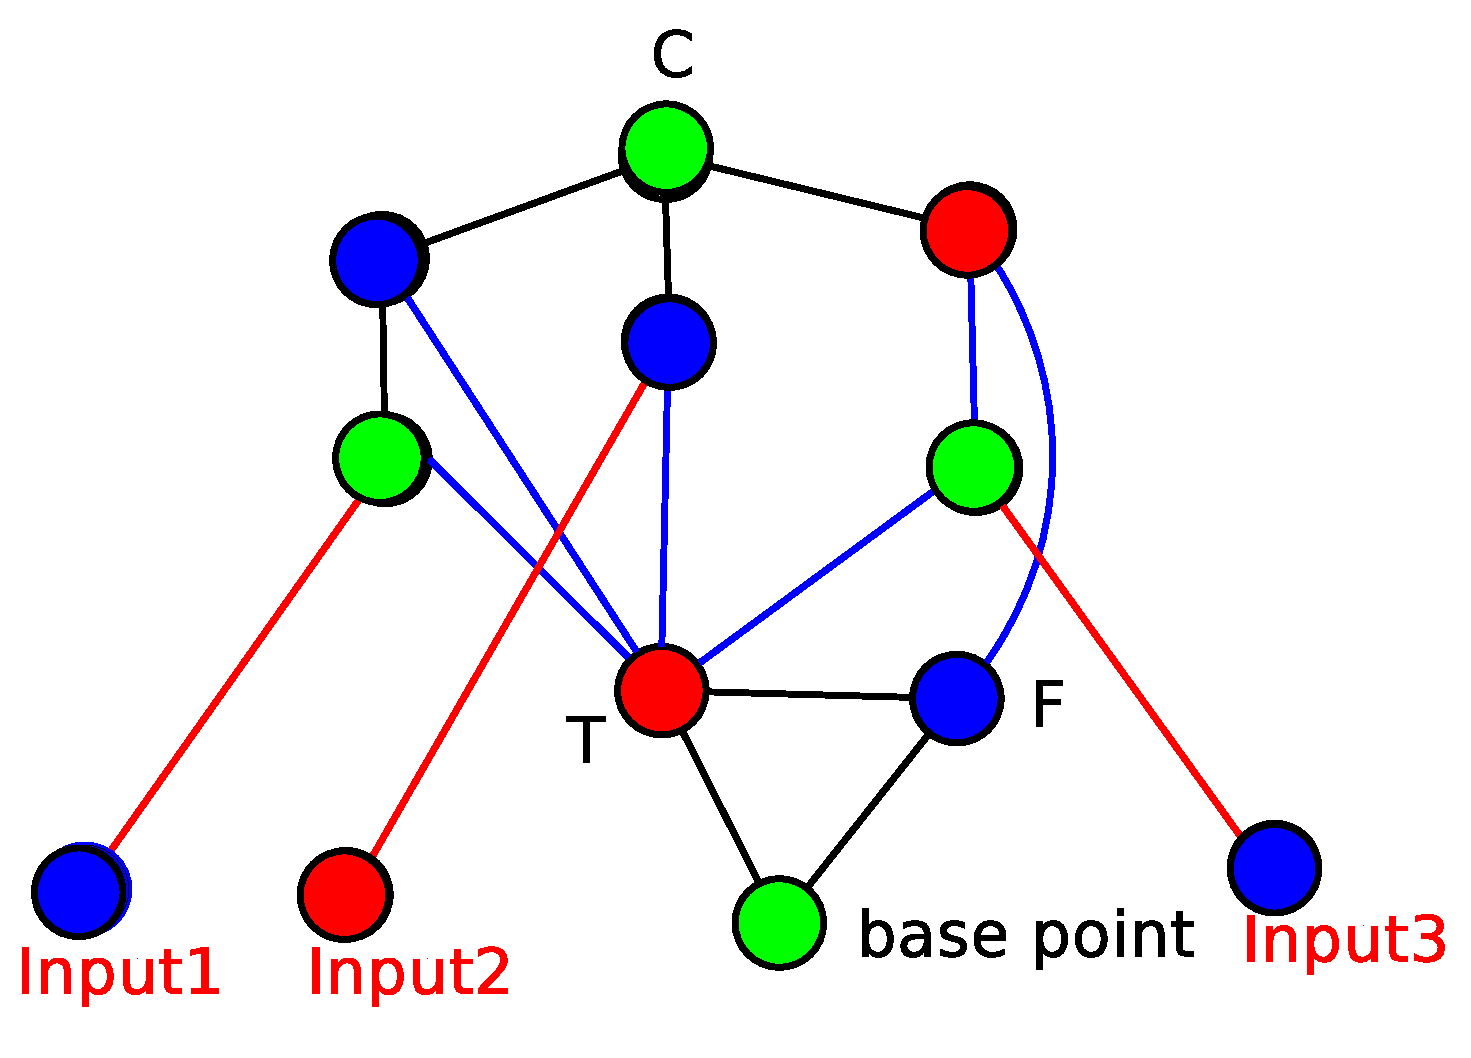
\includegraphics[width=2in] {L3-coloringclausecrownBRB.eps}
\end{figure}

总共八种可能,除了第一个以外,其余的情况都可以,这就是王冠的特性即三个输入至少有一个输入为TRUE才能对节点$C$进行着色。

\subsubsection{归约——变换,等价性}
我们讲完王冠,终于讲到怎么为SAT问题构造一幅图出来。对SAT问题,每个变量构造一个三角形。

\begin{figure}[H]
\centering
 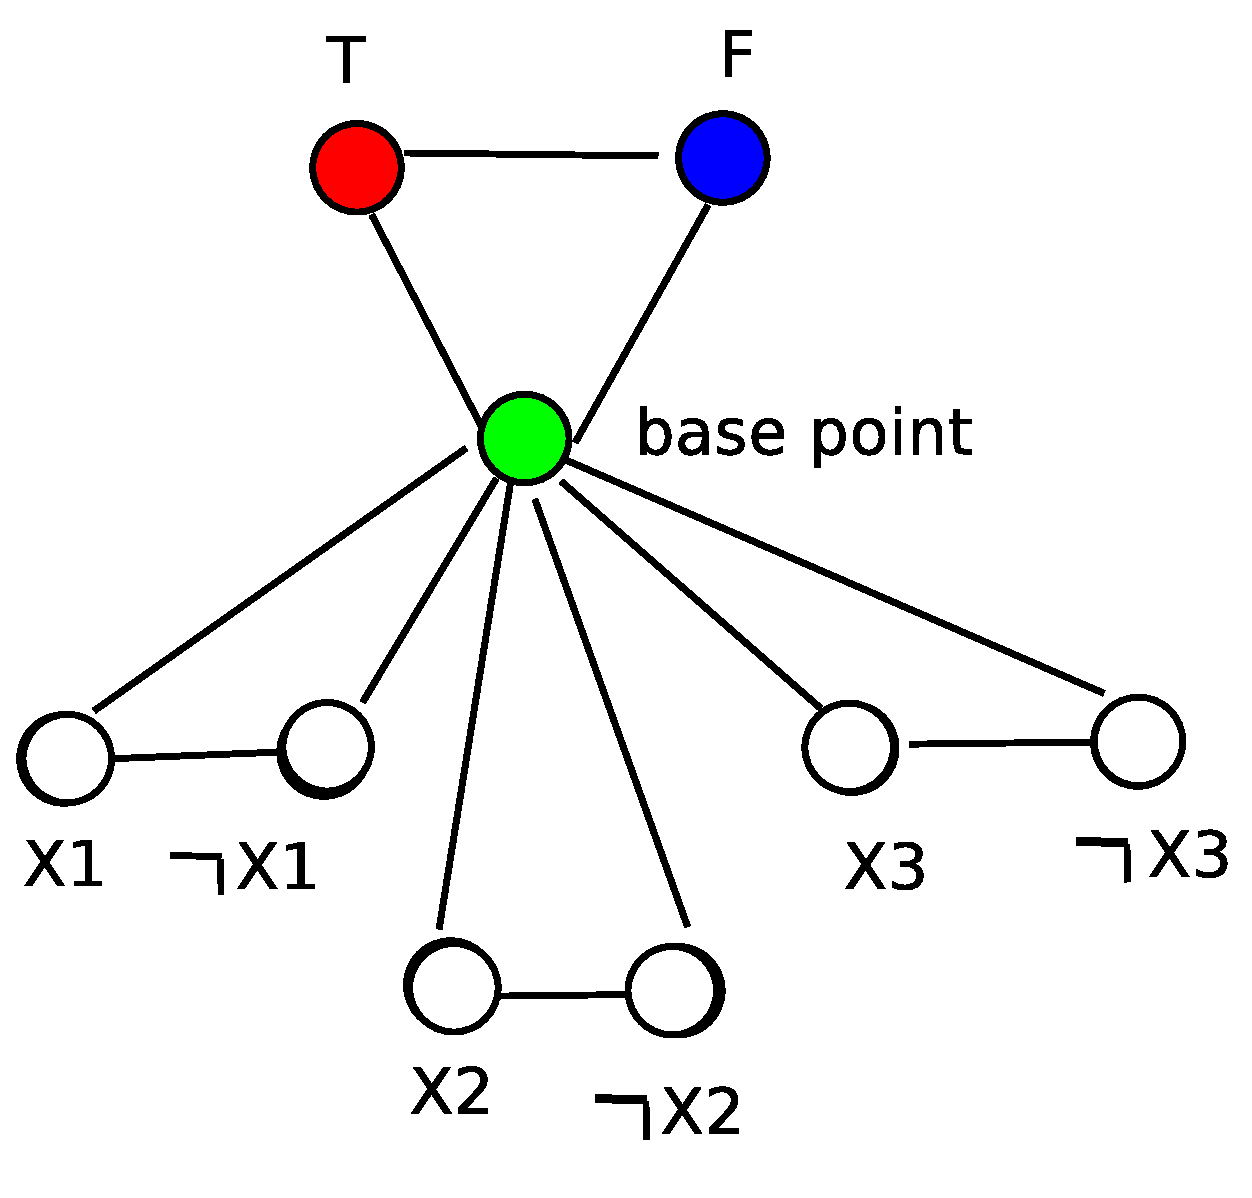
\includegraphics[width=2in] {L3-coloringvariables.eps}
\end{figure}

将基准三角形放在这里后,为每个变量构造一个三角形,即我们为$X_1$构造一个三角形,两个节点$X_1,\neg X_1$都连接到绿色的顶点,第二个三角形是代表$X_2,\neg X_2$的两个节点连接到绿色的顶点,变量$X_3$同理构造。所以我们如果给第一个三角形左边的代表$X_1$的节点着红色,则我们只能给旁边的代表$\neg X_1$的顶点着蓝色,反之亦然,假如红色表示TRUE,则第一个三角形可以表示要么$X_1=\texttt{TRUE}$,要么$\neg X_1 = \texttt{TRUE}$。任何一个变量我们都可以按照这种方式进行分析。

接着我们怎么对子句进行构造呢?假如给我们一个SAT问题的实例,这个实例只有一个子句$C = (x_1 \vee \neg x_2 \vee x_3)$,我们先画一个王冠放在上部,基准三角形也是固定的,并且王冠和基准三角形要进行相对应的连接。我们注意到子句中第一个文字是$X_1$,则第一个输入也指向$X_1$,同理第二个输入连向$\neg X_2$,第三个输入指向$X_3$。

\begin{figure}[H]
\centering
 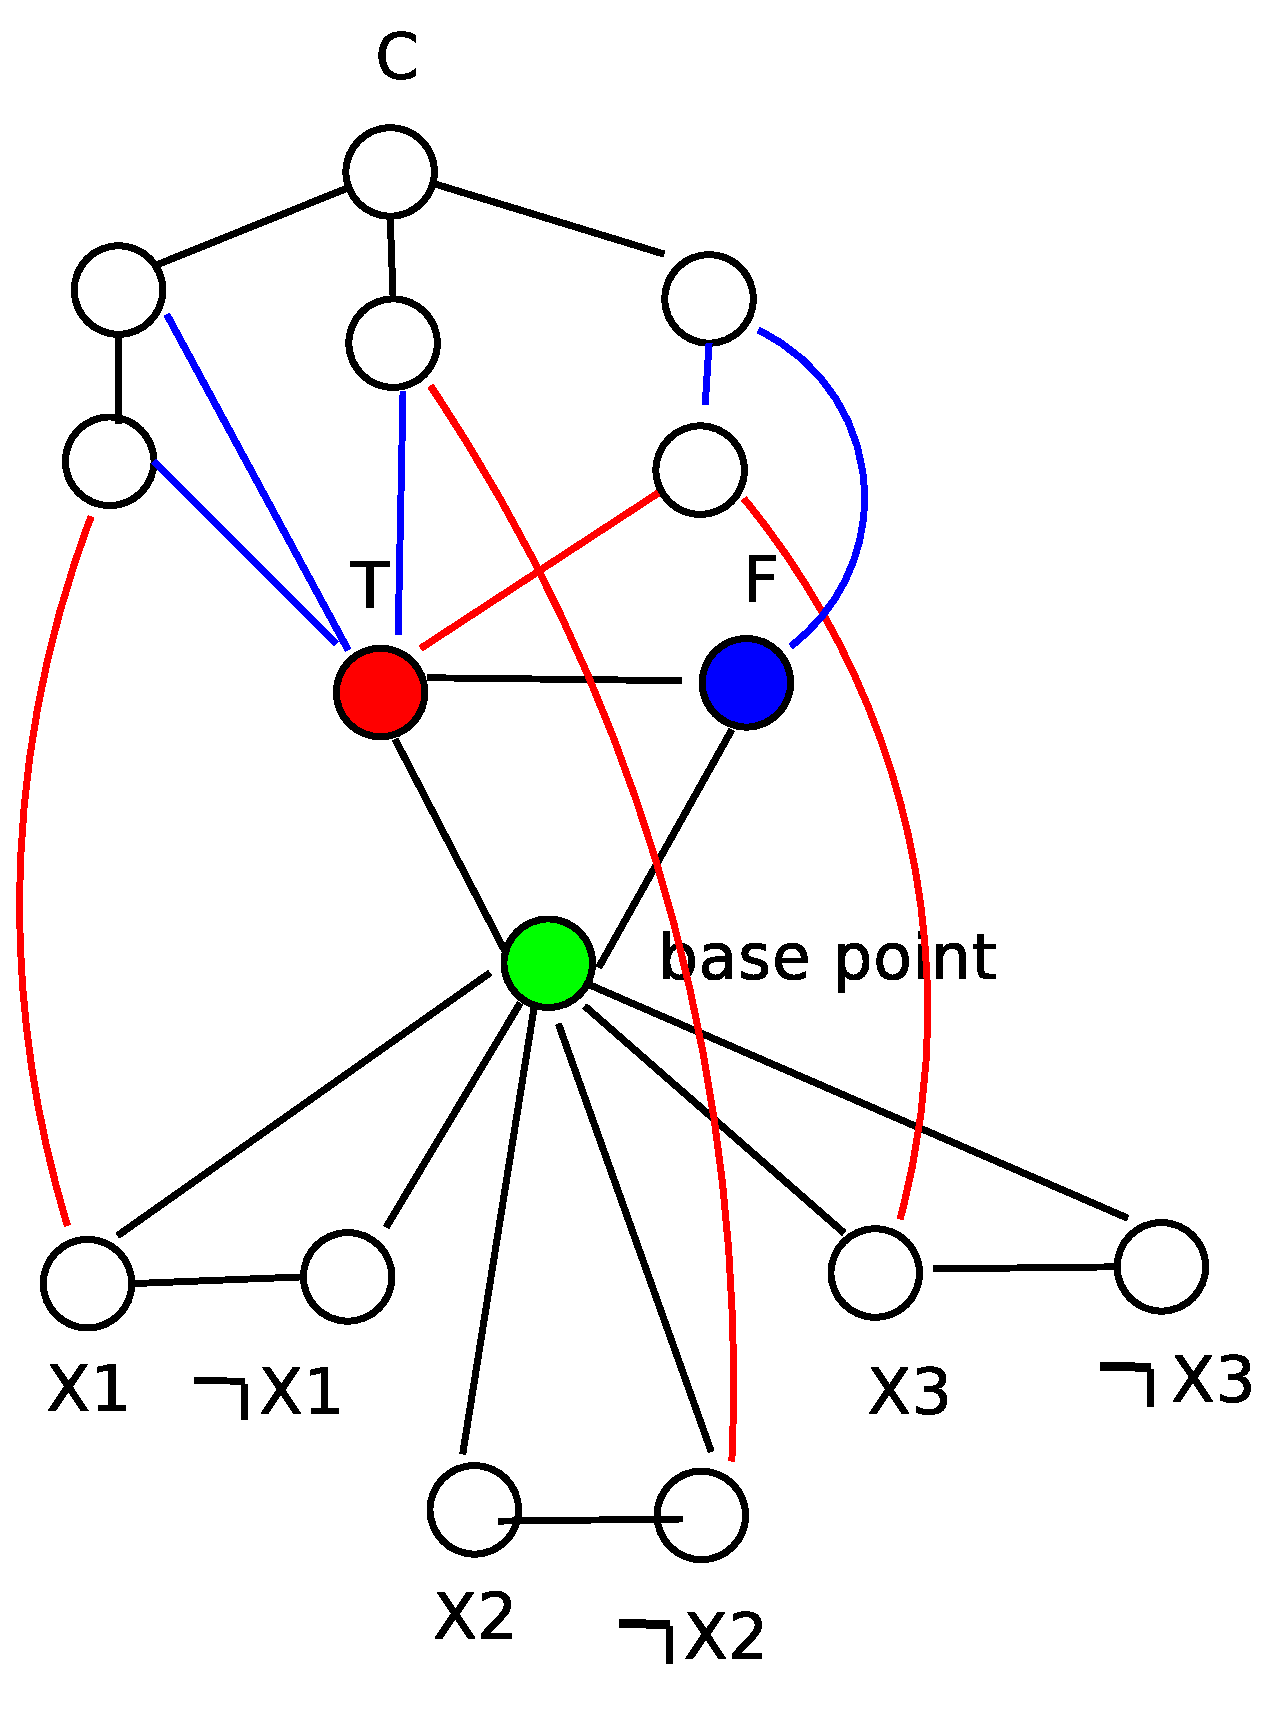
\includegraphics[width=1.5in] {L3-coloringclause.eps}
\end{figure}

最后我们只要说一句话就行了,子句假如是可满足的话,则对应的图必定存在一种着色方案,进行3着色。下面是一个3着色的例子。

 \begin{figure}[H]
 \centering
  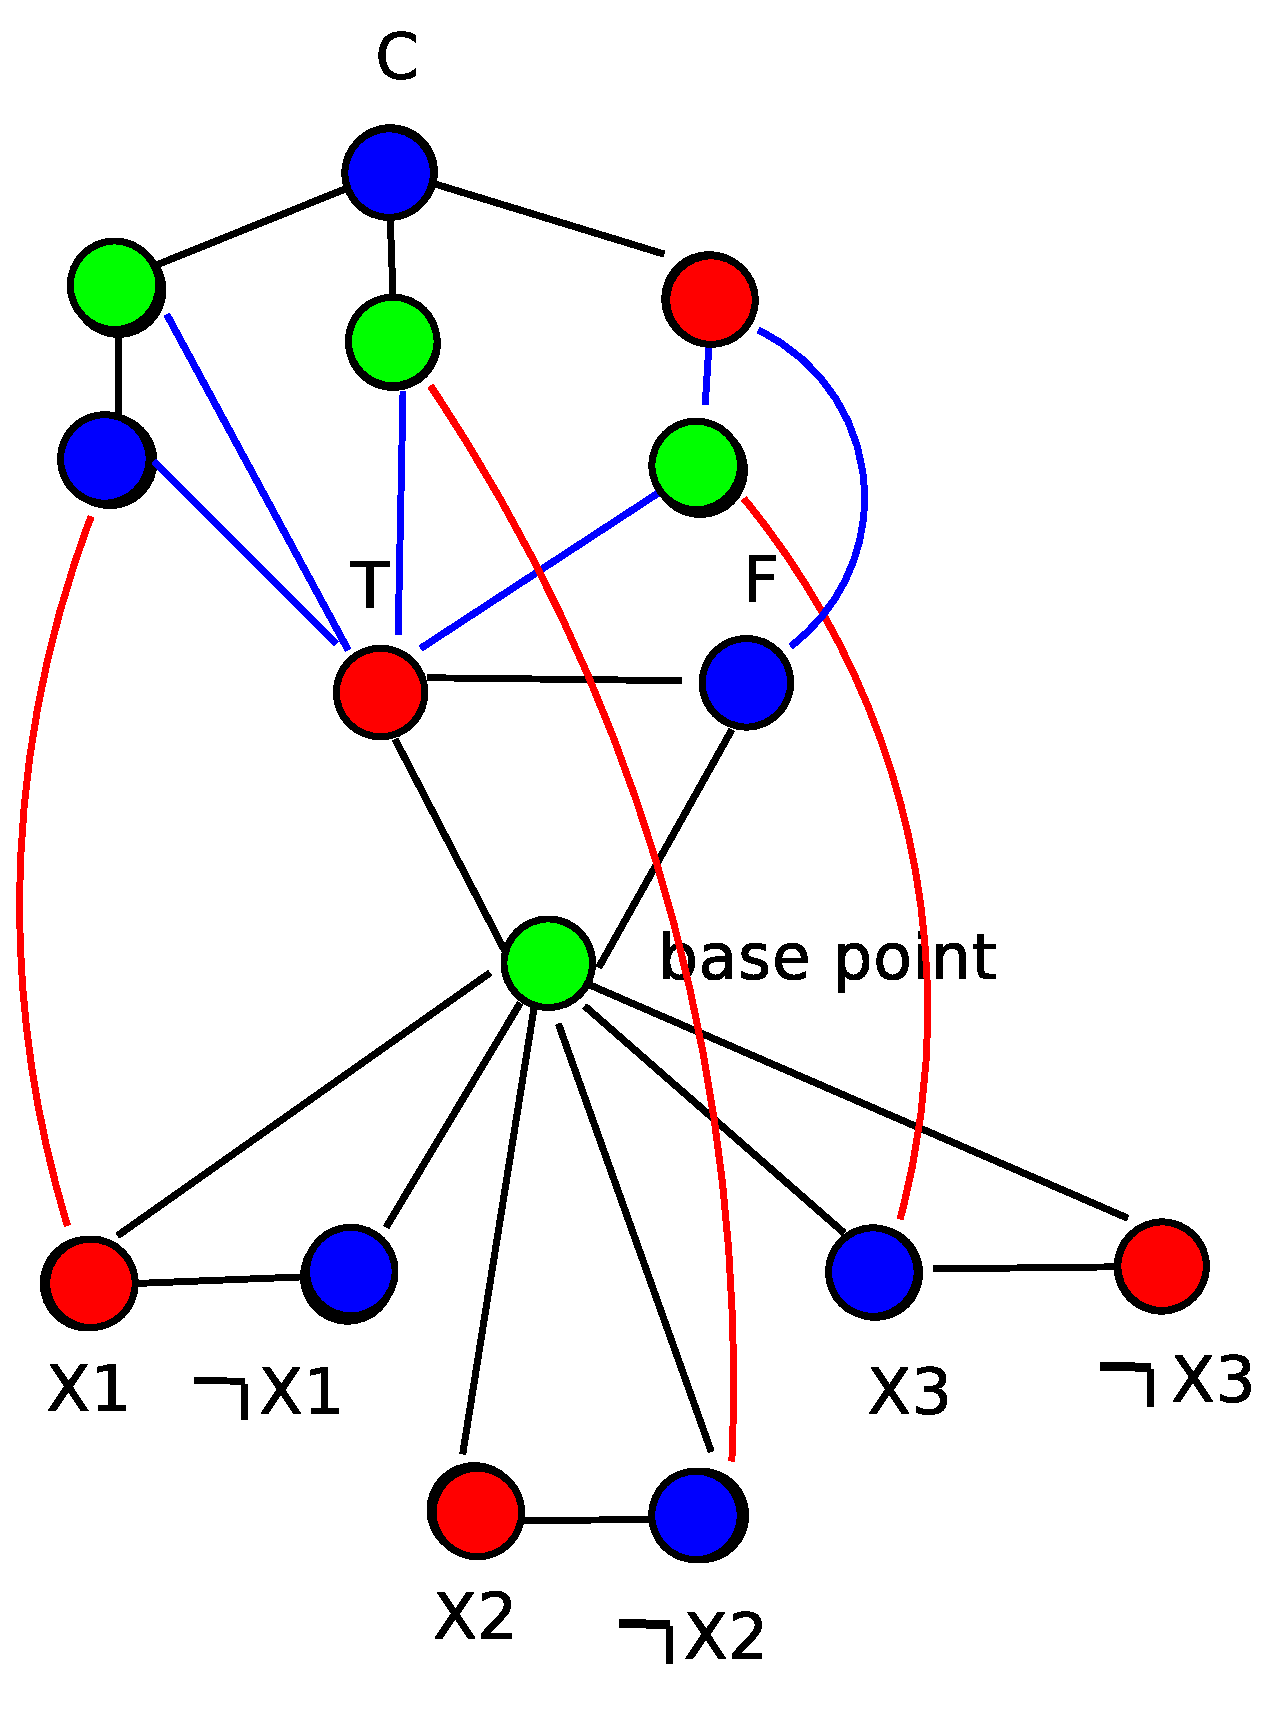
\includegraphics[width=1.8in] {L3-coloringclause-satcase1.eps}
 \end{figure}

在这个结果中,我们令$X_1 = \texttt{TRUE},X_2 = \texttt{TRUE},X_3 = \texttt{FALSE}$,子句的确是可满足的,则在对应的图中,我们令$X_1,X_2,\neg X_3$三个对应的节点为红色,其余为蓝色。通过观察我们可以发现,三个输入不都为蓝色,所以可以对节点$C$进行着色。那么假如赋值导致子句是FALSE,即$X_1 = \texttt{FALSE},X_2 = \texttt{TRUE},X_3 = \texttt{TRUE}$,所以在对应的图中,$X_1,X_2,\neg X_3$对应的节点为蓝色,其余为红色。因为三个输入均为蓝色,所以节点$C$不可能进行着色。

以上分析说明了,对于任意一个SAT问题的实例,我们就能构造一个精巧的图,假如不把颜色告诉大家,让大家对这个图进行着色,任意一条边两个端点不会有同一个颜色。假如你在这种情况下能找到一种着色方案,你就能解决SAT问题。事实上SAT问题是非常非常难的,下堂课我们再介绍为什么说SAT问题非常非常难。

%\end{document}